\documentclass[a4paper,12pt]{report}
\usepackage[left=3cm,right=2.5cm,top=2.5cm,bottom=2.5cm]{geometry}
\usepackage[LGR,T1]{fontenc}
\usepackage[utf8]{inputenc}
\usepackage[english,greek]{babel}
\usepackage{amsmath,amsfonts,amssymb}
\usepackage[parfill]{parskip}
\usepackage[unicode,hidelinks]{hyperref}
\usepackage{bookmark}
\usepackage{cite}
\usepackage{graphicx}
\usepackage{subcaption}
\usepackage{float}
\usepackage{siunitx}
\usepackage{booktabs}
\usepackage{array}
\usepackage{listings}
\usepackage{color}
\usepackage{kmath,kerkis}
\usepackage{textgreek}
\graphicspath{{../PICS/}}

\def\tl{\textlatin}
\def\tg{\textgreek}
\newcommand{\en}[1]{\textlatin{#1}}
\newcommand{\greekbibliographytitle}{Βιβλιογραφία}
\renewcommand{\contentsname}{Περιεχόμενα}
\renewcommand{\listfigurename}{Κατάλογος Σχημάτων}
\renewcommand{\lstlistingname}{Λίστα}
\addto\captionsenglish{\renewcommand{\bibname}{\greekbibliographytitle}}
\addto\captionsgreek{\renewcommand{\bibname}{\greekbibliographytitle}}
\newcommand{\figureplaceholder}[2][0.82\textwidth]{%
  \fbox{%
    \begin{minipage}[c][0.2\textheight][c]{#1}
      \centering \small #2
    \end{minipage}%
  }%
}
\lstdefinelanguage{javascript}{
  basicstyle=\ttfamily\small,
  showstringspaces=false,
  breaklines=true
}
\lstdefinelanguage{json}{
  basicstyle=\ttfamily\small,
  showstringspaces=false,
  breaklines=true
}
\lstset{
  basicstyle=\fontencoding{T1}\ttfamily\small,
  columns=fullflexible,
  keepspaces=true,
  breaklines=true,
  showstringspaces=false,
  frame=single
}

\begin{document}

\pagenumbering{roman}
\setcounter{page}{1}
\begin{titlepage}

\begin{figure}[H]
  \begin{center}
    
\includegraphics[width=3cm]{auth.pdf}
    \label{fig:cover_auth_logo}
  \end{center}
\end{figure}

\centering
\Large Αριστοτέλειο Πανεπιστήμιο Θεσσαλονίκης\\
\Large Πολυτεχνική Σχολή\\
\large Τμήμα Ηλεκτρολόγων Μηχανικών και Μηχανικών Υπολογιστών\\
\large Τομέας Ηλεκτρονικής \& Υπολογιστών

\vspace{\fill}

\LARGE Ψηφιακά Δίδυμα στην Εκπαίδευση: Ανάπτυξη Συστήματος \textlatin{IoT} για τη Βελτιστοποίηση της Ενεργειακής Απόδοσης και του Μαθησιακού Περιβάλλοντος

\vspace{\fill}

\Large Διπλωματική Εργασία\\
\Large του\\
\Large Αλέξανδρου Παπαδόπουλου

\vspace{\fill}
\raggedright

\begin{tabular}{ll}
\textbf{Επιβλέπων καθηγητής:} & Αλκιβιάδης Χατζόπουλος, Α.Π.Θ.\\
\end{tabular}

\centering
\vspace{\fill}
\today

\end{titlepage}
\setcounter{page}{0}

\chapter*{Περίληψη}
\addcontentsline{toc}{chapter}{Περίληψη}

Η παρούσα διπλωματική εργασία πραγματεύεται τον σχεδιασμό, την υλοποίηση και την αξιολόγηση μιας ολοκληρωμένης πλατφόρμας Ψηφιακού Διδύμου (\textlatin{Digital Twin}), ειδικά προσαρμοσμένης για εκπαιδευτικά περιβάλλοντα και Έξυπνες Πανεπιστημιουπόλεις (\textlatin{Smart Campuses}). Σε αντίθεση με τις παραδοσιακές, αντιδραστικές (\textlatin{reactive}) μεθόδους διαχείρισης κτιρίων ή τα απλά συστήματα παρακολούθησης (\textlatin{Digital Shadows}), η προτεινόμενη λύση εγκαθιδρύει μια αμφίδρομη, πραγματικού χρόνου επικοινωνία μεταξύ του φυσικού σχολικού χώρου και του ψηφιακού του αντιγράφου, επιτρέποντας τη λήψη αυτοματοποιημένων αποφάσεων.

Η ανάπτυξη του συστήματος ακολούθησε μια αυστηρή διεπιστημονική προσέγγιση, βασισμένη στην αρχιτεκτονική πέντε επιπέδων. Σε επίπεδο υλικού, εγκαταστάθηκε δίκτυο κόμβων Διαδικτύου των Πραγμάτων (\textlatin{IoT}) χαμηλού κόστους, αποτελούμενο από μικροελεγκτές \textlatin{ESP32}, έξυπνους μετρητές \textlatin{Shelly 1PM} και συσκευές \textlatin{Sonoff}. Σε επίπεδο λογισμικού, αναπτύχθηκε μια ισχυρή, τοπικά εκτελούμενη αρχιτεκτονική με χρήση \textlatin{MQTT, InfluxDB} και \textlatin{openHAB} ως σημασιολογικό ενδιάμεσο λογισμικό (\textlatin{edge middleware}) στο τοπικό επίπεδο, το οποίο τροφοδοτεί ένα \textlatin{Enterprise Cloud SaaS} επίπεδο (\textlatin{React 18 / Supabase}) που υλοποιεί την τελική τρισδιάστατη (\textlatin{3D}) διεπαφή χρήστη.

Η έρευνα δομείται πάνω σε τρεις κεντρικούς πυλώνες: (α) τη βελτιστοποίηση του μαθησιακού περιβάλλοντος (\textlatin{Environmental Quality}), μέσω της διαρκούς παρακολούθησης της ακουστικής άνεσης με επιχειρησιακό όριο παρέμβασης τα \textlatin{55 dBA}, (β) την ενεργειακή αποδοτικότητα (\textlatin{Energy Efficiency}), με συνεχή καταγραφή ισχύος, και (γ) τη λειτουργική διαχείριση (\textlatin{Facility Management}) μέσω απομακρυσμένου ελέγχου. Από την πιλοτική εφαρμογή στα «Εκπαιδευτήρια Πλάτων» (Μάρτιος -- Νοέμβριος 2025), επιτεύχθηκε και επαληθεύτηκε μέση μείωση της ενεργειακής κατανάλωσης κατά 19,7\%. Παράλληλα, η τεχνοοικονομική ανάλυση επιβεβαίωσε την υψηλή προστιθέμενη αξία της μετάβασης σε ένα σύγχρονο Έξυπνο Σχολείο, καταδεικνύοντας απόσβεση της επένδυσης σε 42,5 μήνες και 5ετές \textlatin{ROI} 41,02\%.

\noindent\textbf{Λέξεις-Κλειδιά:} Ψηφιακό Δίδυμο, Έξυπνο Σχολείο, Διαδίκτυο των Πραγμάτων (\textlatin{IoT}), Μαθησιακό Περιβάλλον, Ενεργειακή Αποδοτικότητα, Διαχείριση Εγκαταστάσεων.

\clearpage
\selectlanguage{english}
\chapter*{Abstract}
\addcontentsline{toc}{chapter}{Abstract}

This diploma thesis presents the design, implementation, and evaluation of a comprehensive \textlatin{Digital Twin} platform tailored specifically for educational environments and \textlatin{Smart Campuses}. In contrast to traditional reactive building-management methods or simple monitoring systems (\textlatin{Digital Shadows}), the proposed solution establishes a bidirectional, real-time communication channel between the physical school environment and its digital counterpart, enabling automated decision-making.

The system was developed through a rigorous interdisciplinary approach based on a five-layer architecture. At the hardware level, a low-cost \textlatin{Internet of Things} (\textlatin{IoT}) network was deployed, consisting of ESP32 microcontrollers, Shelly 1PM smart meters, and Sonoff devices. At the software level, a locally executed architecture was implemented using the MQTT protocol, the InfluxDB time-series database, and the open-source openHAB middleware operating as edge semantic middleware, which feeds an Enterprise Cloud SaaS layer (React 18 / Supabase) that delivers the final three-dimensional (3D) user interface.

The research is structured around three core pillars: (\textlatin{a}) optimization of the learning environment (\textlatin{Environmental Quality}) through continuous acoustic-comfort monitoring based on a 55 dBA intervention threshold; (\textlatin{b}) \textlatin{Energy Efficiency} through continuous power tracking; and (\textlatin{c}) \textlatin{Facility Management} through centralized monitoring and remote actuation. Following the pilot implementation at Platon Schools (March -- November 2025), an average energy-consumption reduction of 19.7\% was achieved and verified. In parallel, the techno-economic analysis confirmed the added value and financial viability of the proposed approach, demonstrating a 42.5-month payback period and a five-year ROI of 41.02\%.

\noindent\textbf{Keywords:} \textlatin{Digital Twin}, \textlatin{Smart Campus}, \textlatin{Internet of Things} (\textlatin{IoT}), Learning Environment, \textlatin{Energy Efficiency}, \textlatin{Facility Management}.
\selectlanguage{greek}
\clearpage


\chapter*{Ευχαριστίες}
\addcontentsline{toc}{chapter}{Ευχαριστίες}
Η παρούσα διπλωματική εργασία αποτελεί το επιστέγασμα μιας μακράς, απαιτητικής, αλλά και εξαιρετικά δημιουργικής
προσπάθειας. Η ολοκλήρωσή της δεν θα ήταν εφικτή χωρίς την πολύτιμη συμβολή, καθοδήγηση και υποστήριξη ανθρώπων
που στάθηκαν δίπλα μου και πίστεψαν στο όραμα αυτής της πλατφόρμας.

Αρχικά, θα ήθελα να εκφράσω τις θερμότερες και ειλικρινείς ευχαριστίες μου στον επιβλέποντα καθηγητή μου,
κ. Άλκη Χατζόπουλο, για την εμπιστοσύνη που μου έδειξε, την πολύτιμη ακαδημαϊκή του καθοδήγηση και τη συνεχή
υποστήριξη καθ' όλη τη διάρκεια εκπόνησης της εργασίας.

Ένα ξεχωριστό και μεγάλο ευχαριστώ οφείλω στον κ. Χρήστο Κάλλα. Η συμβολή του υπήρξε καθοριστική, καθώς
αποτέλεσε την αφετηρία και την τεχνική βάση ολόκληρης της έρευνας. Η βοήθειά του στην εγκατάσταση του υλικού
εξοπλισμού (\textlatin{hardware}) και των αισθητήρων \textlatin{IoT}, καθώς και η πολύτιμη καθοδήγησή του στο στήσιμο και την
παραμετροποίηση της πλατφόρμας \textlatin{openHAB}, αποτέλεσαν το θεμέλιο πάνω στο οποίο αναπτύχθηκε το παρόν Ψηφιακό
Δίδυμο.

Τέλος, θα ήθελα να ευχαριστήσω θερμά τη διοίκηση, τους εκπαιδευτικούς και το προσωπικό των «Εκπαιδευτηρίων
Πλάτων» στην Κατερίνη. Η προθυμία τους να αποδεχθούν το σχολείο τους ως πεδίο μελέτης περίπτωσης
(\textlatin{case study}) και να φιλοξενήσουν την πιλοτική εφαρμογή του συστήματος, μου έδωσε τη μοναδική ευκαιρία να
εφαρμόσω τη θεωρία στην πράξη σε ένα πραγματικό, ζωντανό εκπαιδευτικό περιβάλλον.

\clearpage


\tableofcontents
\addcontentsline{toc}{chapter}{Περιεχόμενα}
\clearpage

\listoffigures
\addcontentsline{toc}{chapter}{Κατάλογος Σχημάτων}
\clearpage

\listoftables
\addcontentsline{toc}{chapter}{Κατάλογος Πινάκων}
\clearpage

\chapter*{Συντομογραφίες}
\phantomsection
\addcontentsline{toc}{chapter}{Συντομογραφίες}

\selectlanguage{english}
\begin{description}
  \item[\textlatin{AI}] \textlatin{Artificial Intelligence}
  \item[\textlatin{BIM}] \textlatin{Building Information Modeling}
  \item[\textlatin{BMS}] \textlatin{Building Management System}
  \item[\textlatin{CAPEX}] \textlatin{Capital Expenditure}
  \item[\textlatin{COTS}] \textlatin{Commercial Off-The-Shelf}
  \item[\textlatin{DT}] \textlatin{Digital Twin}
  \item[\textlatin{HACCP}] \textlatin{Hazard Analysis and Critical Control Points}
  \item[\textlatin{HVAC}] \textlatin{Heating, Ventilation, and Air Conditioning}
  \item[\textlatin{I2S}] \textlatin{Inter-IC Sound}
  \item[\textlatin{IEQ}] \textlatin{Indoor Environmental Quality}
  \item[\textlatin{IoT}] \textlatin{Internet of Things}
  \item[\textlatin{KPI}] \textlatin{Key Performance Indicator}
  \item[\textlatin{LAeq}] \textlatin{Equivalent Continuous Sound Level}
  \item[\textlatin{LLM}] \textlatin{Large Language Model}
  \item[\textlatin{MQTT}] \textlatin{Message Queuing Telemetry Transport}
  \item[\textlatin{MVP}] \textlatin{Minimum Viable Product}
  \item[\textlatin{OPEX}] \textlatin{Operational Expenditure}
  \item[\textlatin{RBAC}] \textlatin{Role-Based Access Control}
  \item[\textlatin{RESTful}] \textlatin{Representational State Transfer architectural style}
  \item[\textlatin{ROI}] \textlatin{Return on Investment}
  \item[\textlatin{SaaS}] \textlatin{Software as a Service}
  \item[\textlatin{SPA}] \textlatin{Single Page Application}
  \item[\textlatin{UI}] \textlatin{User Interface}
  \item[\textlatin{VL}] \textlatin{Virtual Layer}
  \item[\textlatin{WHO}] \textlatin{World Health Organization}
  \item[\textlatin{YoY}] \textlatin{Year-over-Year}
\end{description}
\selectlanguage{greek}

\noindent\textit{Σημείωση: Η πλατφόρμα Ψηφιακού Διδύμου που αναπτύχθηκε στο πλαίσιο της παρούσας εργασίας είναι διαθέσιμη στη διεύθυνση: \href{https://digitaltwin.pi-tech.gr}{https://digitaltwin.pi-tech.gr}}


\clearpage
\pagenumbering{arabic}
\setcounter{page}{1}

\chapter{Εισαγωγή}

\section{Επιστημονική Περιοχή της Διπλωματικής}
Η ραγδαία εξέλιξη του Διαδικτύου των Πραγμάτων (\textlatin{Internet of Things - IoT}) και των υπολογιστικών υποδομών παρυφής (\textlatin{Edge Computing}) έχει οδηγήσει στην ανάδυση της τεχνολογίας των Ψηφιακών Διδύμων (\textlatin{Digital Twins}). Στη σύγχρονη βιβλιογραφία, ένα Ψηφιακό Δίδυμο ορίζεται ως η δυναμική, εικονική αναπαράσταση ενός φυσικού αντικειμένου, συστήματος ή διαδικασίας, η οποία τροφοδοτείται με δεδομένα πραγματικού χρόνου και επιτρέπει την προσομοίωση, την παρακολούθηση και, το σημαντικότερο, τον αμφίδρομο έλεγχο \cite{Grieves2017}, \cite{Han2022}.

Η μετάβαση από το απλό 'Ψηφιακό Μοντέλο' (\textlatin{Digital Model}) στην 'Ψηφιακή Σκιά' (\textlatin{Digital Shadow}) και, τελικά, στο πλήρες 'Ψηφιακό Δίδυμο', αποτελεί αντικείμενο εκτενούς έρευνας. Παράλληλα, σε ευρωπαϊκό επίπεδο, πρωτοβουλίες όπως το πρόγραμμα \textit{\textlatin{DIGITAL EUROPE}} επενδύουν στρατηγικά στη δημιουργία Τοπικών Ψηφιακών Διδύμων (\textlatin{Local Digital Twins}) για την ενίσχυση της βιωσιμότητας και της λειτουργικότητας των έξυπνων κοινοτήτων \cite{EuropeanCommission2023}. Η παρούσα διπλωματική εργασία εντάσσεται στον ευρύτερο ερευνητικό τομέα των Έξυπνων Κτιριακών Υποδομών (\textlatin{Smart Buildings}) και ειδικότερα στην εξειδίκευση των Έξυπνων Πανεπιστημιουπόλεων και Σχολείων (\textlatin{Smart Campuses}), μελετώντας την ενσωμάτωση του IoT στην εκπαιδευτική διαδικασία και τη λειτουργική διαχείριση (\textlatin{Facility Management}) \cite{Balla2023, Barros2024, Evangelou2022, Cui2023, EUParliament2024}.

\section{Σκοπός και Συνεισφορά της Διπλωματικής}
Σκοπός της παρούσας διπλωματικής εργασίας είναι ο σχεδιασμός, η υλοποίηση και η τεχνοοικονομική αξιολόγηση μιας ολοκληρωμένης πλατφόρμας Ψηφιακού Διδύμου, προσαρμοσμένης αποκλειστικά για σχολικά κτίρια. Ως πεδίο εφαρμογής (\textlatin{Case Study}) επιλέχθηκαν τα «Εκπαιδευτήρια Πλάτων» στην Κατερίνη.

Σε αντίθεση με συμβατικά συστήματα τηλεμετρίας, το προτεινόμενο σύστημα εγκαθιδρύει έναν κλειστό βρόχο αλληλεπίδρασης (\textlatin{Sense - Decide - Act}) μεταξύ του φυσικού και του ψηφιακού χώρου. Το σύστημα αναπτύχθηκε με χρήση ανοιχτού κώδικα (\textlatin{openHAB} ως \textlatin{semantic middleware}) και IoT εξοπλισμό χαμηλού κόστους (όπως μικροελεγκτές \textlatin{ESP32}, έξυπνους μετρητές \textlatin{Shelly 1PM} και ρελέ \textlatin{Sonoff}), που επικοινωνούν μέσω του πρωτοκόλλου \textlatin{MQTT}. Το σύστημα εξελίχθηκε σε ένα \textlatin{Enterprise Cloud SaaS} περιβάλλον (\textlatin{React 18}, \textlatin{Supabase}), το οποίο παρέχει την τελική εμπειρία χρήστη με \textlatin{responsive} πρόσβαση, \textlatin{3D} οπτικοποίηση και πολυεπίπεδο έλεγχο πρόσβασης.

Η κύρια συνεισφορά της εργασίας εστιάζεται σε τρεις άξονες:
\begin{itemize}
\item \textbf{Ποιότητα Εσωτερικού Περιβάλλοντος (\textlatin{IEQ}) και Μάθηση:} Η δυναμική παρακολούθηση της ακουστικής άνεσης στις αίθουσες διδασκαλίας (διατηρώντας τα επίπεδα κάτω από το όριο των 55~\textlatin{dBA}) με χρήση διακριτικής οπτικής ανατροφοδότησης (\textlatin{quiet-lamp}) προς τους μαθητές, προστατεύοντας την εκπαιδευτική διαδικασία \cite{WHO1999, Kephalopoulos2015}.
\item \textbf{Ενεργειακή Αποδοτικότητα:} Η βελτιστοποίηση της λειτουργίας ηλεκτροβόρων συσκευών, κυρίως στον χώρο του κυλικείου, που οδήγησε σε επαληθευμένη μείωση της ενεργειακής κατανάλωσης κατά 19,7\%.
\item \textbf{Λειτουργική Διαχείριση (\textlatin{Facility Management}):} Η ανάπτυξη ενός κεντρικού συστήματος τρισδιάστατης οπτικοποίησης (\textlatin{React 3D Dashboard}) και παρακολούθησης της ασφάλειας (π.χ. κατάσταση θυρών ψυγείων, έλεγχος πρόσβασης πυλών), επιτρέποντας την προγνωστική συντήρηση.
\end{itemize}

Η βασική ερευνητική υπόθεση (\textlatin{research hypothesis}) της παρούσας μελέτης είναι ότι η μετάβαση από ένα παθητικό σύστημα παρακολούθησης σε ένα ενεργό Ψηφιακό Δίδυμο (\textlatin{Digital Twin}) μπορεί να επιφέρει άμεση και μετρήσιμη βελτίωση στις λειτουργικές παραμέτρους μιας σχολικής υποδομής. Ειδικότερα, εξετάζεται (α) εάν ο αμφίδρομος έλεγχος μπορεί να διατηρήσει τα επίπεδα θορύβου κάτω από το όριο των 55~\textlatin{dBA} προστατεύοντας τη μαθησιακή διαδικασία, (β) εάν επιτυγχάνεται σημαντική μείωση της μέσης ημερήσιας κατανάλωσης ενέργειας (\textlatin{kWh}/ημέρα), και (γ) εάν η τεχνοοικονομική ανάλυση αποδεικνύει υψηλή απόδοση επένδυσης (\textlatin{ROI}) και ταχεία απόσβεση, επιβεβαιώνοντας την εμπορική βιωσιμότητα της πλατφόρμας.

Η αναπτυχθείσα πλατφόρμα είναι διαθέσιμη σε λειτουργία πραγματικού χρόνου στη διεύθυνση \href{https://digitaltwin.pi-tech.gr}{\textlatin{digitaltwin.pi-tech.gr}}, παρέχοντας δημόσια πρόσβαση σε επιλεγμένες προβολές της αρχιτεκτονικής και των ευρημάτων της έρευνας, καθώς και πλήρη λειτουργική πρόσβαση μέσω διαπιστευτηρίων για εξουσιοδοτημένους χρήστες. Μια επισκόπηση της κεντρικής διεπαφής της πλατφόρμας παρουσιάζεται στο Σχήμα~\ref{fig:dashboard_overview}.

\begin{figure}[htbp]
\centering
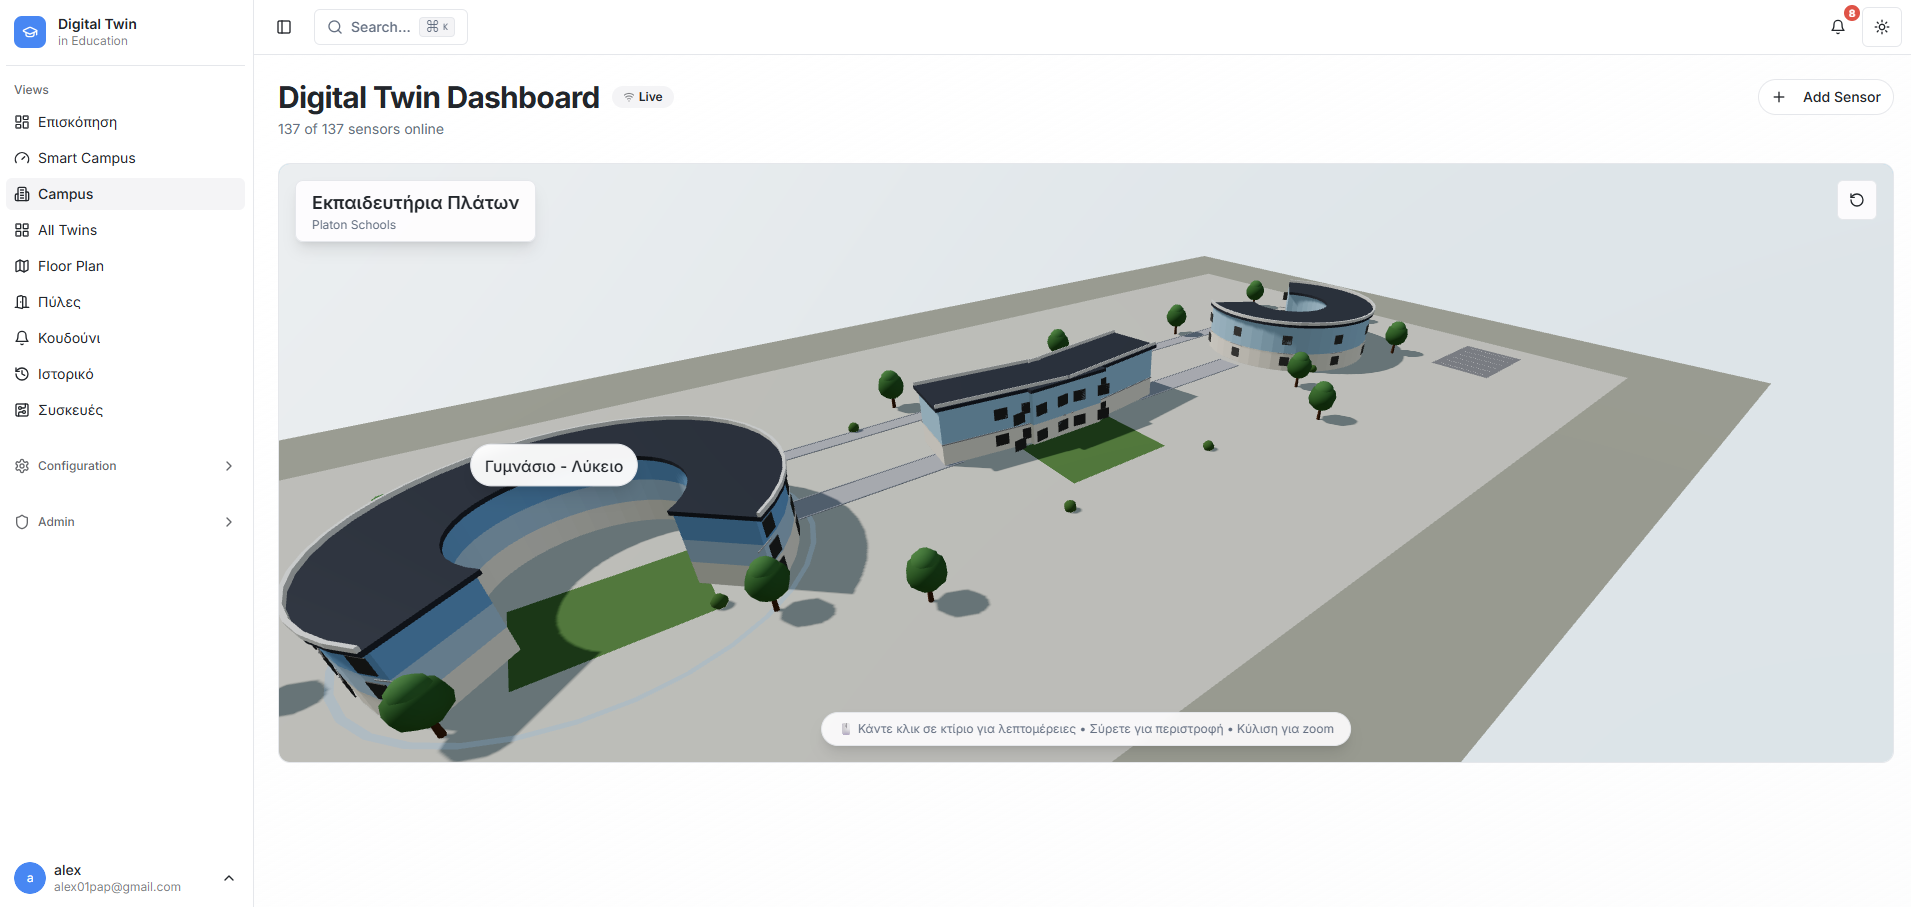
\includegraphics[width=\textwidth]{fig_1_1}
\caption{Επισκόπηση της διεπαφής της προτεινόμενης πλατφόρμας Ψηφιακού Διδύμου}
\label{fig:dashboard_overview}
\end{figure}

\section{Διάρθρωση της Διπλωματικής}
Η παρούσα διπλωματική εργασία αναπτύσσεται σε οκτώ (8) κεφάλαια, τα οποία διαρθρώνονται ως εξής:

Στο \textbf{Κεφάλαιο 1} (παρόν κεφάλαιο) γίνεται η εισαγωγή στο αντικείμενο, καθορίζεται ο σκοπός και παρουσιάζεται η δομή της μελέτης.

Στο \textbf{Κεφάλαιο 2} αναλύεται το θεωρητικό υπόβαθρο και το συναφές έργο γύρω από τα Ψηφιακά Δίδυμα στην εκπαίδευση, την Ποιότητα Εσωτερικού Περιβάλλοντος και τα πρωτόκολλα επικοινωνίας \textlatin{IoT}.

Το \textbf{Κεφάλαιο 3} περιγράφει την Αρχιτεκτονική του Συστήματος βάσει του μοντέλου των 5 επιπέδων, παρουσιάζοντας τον σχεδιασμό του υλικού (\textlatin{Hardware}) και τον διαχωρισμό \textlatin{Digital Shadow} και \textlatin{Digital Twin}.

Το \textbf{Κεφάλαιο 4} εμβαθύνει στην Τεχνική Υλοποίηση του λογισμικού, αναλύοντας τις δύο φάσεις υλοποίησης: το τοπικό πρωτότυπο (\textlatin{openHAB} / \textlatin{InfluxDB} / \textlatin{Grafana}) και την \textlatin{Enterprise Cloud SaaS} πλατφόρμα (\textlatin{React 18}, \textlatin{Supabase}, \textlatin{3D WebGL}).

Στο \textbf{Κεφάλαιο 5} παρουσιάζεται η μεθοδολογία αξιολόγησης του συστήματος στο πραγματικό περιβάλλον του σχολείου, εξηγώντας τον τρόπο μέτρησης της ενέργειας, της ακουστικής και της τεχνοοικονομικής ανάλυσης.

Το \textbf{Κεφάλαιο 6} παραθέτει τα πρακτικά αποτελέσματα (μείωση κατανάλωσης, εξοικονόμηση, βελτίωση ηχητικού περιβάλλοντος) και την τεχνοοικονομική μελέτη (Υπολογισμός \textlatin{ROI}).

Το \textbf{Κεφάλαιο 7} αφορά τη συζήτηση των ευρημάτων, προχωρώντας σε κριτική αξιολόγηση και ερμηνεία των αποτελεσμάτων.

Τέλος, στο \textbf{Κεφάλαιο 8} συνοψίζονται τα τελικά συμπεράσματα της έρευνας, καταγράφονται οι περιορισμοί και προτείνονται κατευθύνσεις για μελλοντική επέκταση της πλατφόρμας.






\chapter{Ανασκόπηση Βιβλιογραφίας και Θεωρητικό Υπόβαθρο}

\section{Εισαγωγή στην Τεχνολογία των Ψηφιακών Διδύμων (\textlatin{Digital Twins})}
Η έννοια του Ψηφιακού Διδύμου (\textlatin{Digital Twin - DT}) έχει αναδειχθεί την τελευταία δεκαετία ως μία από τις πλέον επιδραστικές τεχνολογίες στον τομέα της 4ης Βιομηχανικής Επανάστασης (\textlatin{Industry 4.0}) και του Διαδικτύου των Πραγμάτων (\textlatin{IoT}). Παρότι οι ρίζες της τεχνολογίας εντοπίζονται στον τομέα της αεροδιαστημικής (\textlatin{NASA}) για την παρακολούθηση απομακρυσμένων διαστημικών σκαφών, η ραγδαία εξέλιξη των υπολογιστικών συστημάτων και η μείωση του κόστους των αισθητήρων επέτρεψαν τη μετάβασή της στον κτιριακό και εκπαιδευτικό τομέα.

\subsection{Η Εξέλιξη: Από το Ψηφιακό Μοντέλο στο Ψηφιακό Δίδυμο}
Στη σύγχρονη ακαδημαϊκή βιβλιογραφία, αποτελεί συχνό φαινόμενο η σύγχυση και η εσφαλμένη ταύτιση της απλής τρισδιάστατης μοντελοποίησης με τα πραγματικά Ψηφιακά Δίδυμα. Προκειμένου να τεθεί ένα σαφές ερευνητικό πλαίσιο, είναι απαραίτητος ο αυστηρός εννοιολογικός διαχωρισμός των βαθμίδων ψηφιακής αναπαράστασης, ο οποίος βασίζεται αποκλειστικά στη ροή των δεδομένων (\textlatin{data flow}) μεταξύ του φυσικού και του εικονικού αντικειμένου \cite{Grieves2017}, \cite{Kritzinger2018}, \cite{Fuller2020}.

\begin{itemize}
\item \textbf{Ψηφιακό Μοντέλο (\textlatin{Digital Model}):} Αποτελεί την ψηφιακή αναπαράσταση ενός υπαρκτού ή μελλοντικού φυσικού συστήματος (όπως ένα αρχιτεκτονικό σχέδιο \textlatin{CAD} ή ένα στατικό μοντέλο \textlatin{BIM}). Η κρίσιμη παράμετρος εδώ είναι ότι δεν υφίσταται καμία απολύτως αυτοματοποιημένη ανταλλαγή δεδομένων μεταξύ του φυσικού και του ψηφιακού αντικειμένου. Κάθε αλλαγή στο ψηφιακό μοντέλο πρέπει να εισαχθεί χειροκίνητα από τον χρήστη.
\item \textbf{Ψηφιακή Σκιά (\textlatin{Digital Shadow}):} Πρόκειται για την εξέλιξη του ψηφιακού μοντέλου, όπου εγκαθιδρύεται μια αυτοματοποιημένη, μονόδρομη ροή δεδομένων από το φυσικό αντικείμενο προς το ψηφιακό. Τα περισσότερα σύγχρονα συστήματα τηλεμετρίας, όπως τα \textlatin{dashboards} που παρακολουθούν παραμέτρους (π.χ. θερμοκρασία, κατανάλωση) σε πραγματικό χρόνο, κατατάσσονται σε αυτή την κατηγορία. Μια μεταβολή στη φυσική κατάσταση (π.χ. αύξηση της θερμοκρασίας) αντικατοπτρίζεται αυτόματα στο ψηφιακό ταμπλό, αλλά το σύστημα αδυνατεί να επιδράσει αντίστροφα στο φυσικό περιβάλλον.
\item \textbf{Ψηφιακό Δίδυμο (\textlatin{Digital Twin}):} Η τρίτη και ανώτατη βαθμίδα απαιτεί την ύπαρξη μιας πλήρως αμφίδρομης, αυτοματοποιημένης ροής δεδομένων. Το ψηφιακό αντικείμενο όχι μόνο λαμβάνει ζωντανά δεδομένα από το φυσικό του αντίστοιχο (\textlatin{Sense}), αλλά είναι σε θέση να αναλύει τα δεδομένα, να λαμβάνει αποφάσεις (\textlatin{Decide}) και να στέλνει πίσω εντολές ενεργοποίησης (\textlatin{Act}), επιφέροντας αλλαγές στο φυσικό περιβάλλον (\textlatin{actuation}). Αυτός ο κλειστός βρόχος ελέγχου (\textlatin{closed-loop control}) είναι η βασική προϋπόθεση για τον χαρακτηρισμό ενός συστήματος ως αυθεντικό Ψηφιακό Δίδυμο.
\end{itemize}

Σύμφωνα με πρόσφατες συνθετικές ανασκοπήσεις της βιβλιογραφίας \cite{Han2022, Kritzinger2018}, το μέλλον των Ψηφιακών Διδύμων ξεφεύγει από την απλή οπτικοποίηση. Η ακαδημαϊκή έρευνα συγκλίνει στο ότι η επόμενη γενιά συστημάτων θα βασίζεται σε τέσσερις πυλώνες: την ενσωμάτωση φωνητικών βοηθών (\textlatin{Voice Assistants}), τη συνεχή βελτιστοποίηση υλικού και λογισμικού, την προγνωστική ανάλυση (\textlatin{Predictive Analytics}) μέσω Μηχανικής Μάθησης, με ενδεικτικές εφαρμογές όπως το \textlatin{AI Energy Forecasting}, και, τελικά, την πλήρη αυτονομία στη λήψη αποφάσεων, δηλαδή τη μετάβαση προς γνωστικά Ψηφιακά Δίδυμα (\textlatin{Cognitive Digital Twins}) \cite{Han2022}, \cite{Semeraro2021}. Στο πλαίσιο αυτό, η ανάλυση δεδομένων (\textlatin{Data Analysis}) αποκτά κεντρικό ρόλο, καθώς το \textlatin{AI} μπορεί να επεξεργάζεται πολύ μεγάλους όγκους τηλεμετρίας που συλλέγονται από το φυσικό αντικείμενο, να εντοπίζει κρυφά μοτίβα λειτουργίας και να υποστηρίζει τη βελτιστοποίηση της απόδοσής του. Για παράδειγμα, εάν το ψηφιακό δίδυμο ενός βιομηχανικού ψυγείου εντοπίσει ασυνήθιστους κραδασμούς ή θερμικές διακυμάνσεις, οι αλγόριθμοι \textlatin{AI} μπορούν να αναλύσουν τα σχετικά δεδομένα και να προβλέψουν πιθανές βλάβες πριν αυτές συμβούν, ενισχύοντας πρακτικά την προγνωστική συντήρηση. Παράλληλα, η διαδραστική επικοινωνία (\textlatin{Interactive Communication}) μετασχηματίζει τη σχέση του χρήστη με την πλατφόρμα, αφού αντί για αποκλειστική ανάγνωση στατικών γραφημάτων καθίσταται εφικτή η αλληλεπίδραση μέσω καθημερινής γλώσσας με χρήση τεχνικών επεξεργασίας φυσικής γλώσσας (\textlatin{Natural Language Processing - NLP}). Η προοπτική αυτή έχει ιδιαίτερη σημασία για τις σχολικές και κτιριακές εφαρμογές, καθώς μετατοπίζει το κέντρο βάρους από την παθητική αναπαράσταση του χώρου προς την ενεργή υποστήριξη της λειτουργίας, της βελτιστοποίησης και της επιχειρησιακής διαχείρισής του.

\subsection{Η Αρχιτεκτονική Πέντε Επιπέδων (\textlatin{5-Layer Architecture})}
Για την επιτυχή υλοποίηση ενός Ψηφιακού Διδύμου σε πολύπλοκα περιβάλλοντα, όπως είναι ένα σχολικό συγκρότημα (\textlatin{Smart Campus}), Η αρχιτεκτονική πέντε επιπέδων που υιοθετείται στην παρούσα εργασία βασίζεται στη σύνθεση των προτύπων που προτείνουν οι Han et al. \cite{Han2022} για έξυπνες πανεπιστημιουπόλεις και οι Fuller et al. \cite{Fuller2020} για Ψηφιακά Δίδυμα γενικότερα, αξιοποιώντας την ιεράρχηση \textlatin{Physical, Connection, Data, Virtual} και \textlatin{Service layers} με αμφίδρομη ροή \textlatin{Sense~$\uparrow$ / Act~$\downarrow$}. Το μοντέλο αυτό διασφαλίζει την επεκτασιμότητα (\textlatin{scalability}) και τη διαλειτουργικότητα (\textlatin{interoperability}) των συστημάτων. Τα επίπεδα αυτά περιλαμβάνουν: (1) το \textit{Φυσικό Επίπεδο (\textlatin{Physical Layer})} όπου συλλέγονται τα πρωτογενή δεδομένα μέσω αισθητήρων IoT, (2) το \textit{Επίπεδο Δικτύου (\textlatin{Connection Layer})} που εξασφαλίζει την ασφαλή διακίνηση δεδομένων (π.χ. μέσω \textlatin{MQTT}), (3) την \textit{Πλατφόρμα Δεδομένων (\textlatin{Data Layer})} για την ενοποίηση και αποθήκευση σε βάσεις χρονοσειρών, (4) το \textit{Εικονικό Επίπεδο (\textlatin{Virtual Layer})} που παρέχει την τρισδιάστατη χωρική οπτικοποίηση (\textlatin{3D Models}), και τέλος, (5) το \textit{Επίπεδο Υπηρεσιών (\textlatin{Service Layer})} όπου εκτελούνται οι αλγόριθμοι λήψης αποφάσεων (\textlatin{Rules Engine}) και οι αυτοματισμοί. Η συγκεκριμένη αρχιτεκτονική υιοθετήθηκε πλήρως ως ο κατευθυντήριος άξονας για την ανάπτυξη της πλατφόρμας της παρούσας διπλωματικής εργασίας.

\section{Έξυπνες Πανεπιστημιουπόλεις (\textlatin{Smart Campuses}) και το Ευρωπαϊκό Πλαίσιο}
Η εφαρμογή των Ψηφιακών Διδύμων έχει αρχίσει να μετατοπίζεται από την αμιγώς βιομηχανική παραγωγή (\textlatin{Industry 4.0}) στον αστικό και κτιριακό τομέα, στοχεύοντας στη δημιουργία Έξυπνων Πόλεων (\textlatin{Smart Cities}) και Έξυπνων Σχολικών Υποδομών (\textlatin{Smart Campuses}).

\subsection{Ευρωπαϊκές Πολιτικές και Πρωτοβουλίες}
Η υιοθέτηση των ψηφιακών διδύμων ευθυγραμμίζεται σε μεγάλο βαθμό με τους στρατηγικούς στόχους της Ευρωπαϊκής Ένωσης. Το πρόγραμμα \textit{DIGITAL EUROPE} δίνει ρητή έμφαση στη δημιουργία ``Τοπικών Ψηφιακών Διδύμων'' (Local Digital Twins) ως βασικό εργαλείο για την ενίσχυση της βιωσιμότητας των έξυπνων κοινοτήτων και την αποτελεσματικότερη διαχείριση κτιριακών υποδομών \cite{EuropeanCommission2023}. Επιπρόσθετα, η Ευρωπαϊκή Πράσινη Συμφωνία καθιστά επιτακτική την ενεργειακή αναβάθμιση του κτιριακού αποθέματος \cite{EUParliament2024}. Η ενσωμάτωση τεχνολογιών \textlatin{IoT} σε σχολεία αποτελεί ένα καίριο βήμα για τη μετάβαση σε υποδομές μηδενικών εκπομπών.
Η υιοθέτηση των ψηφιακών διδύμων ευθυγραμμίζεται σε μεγάλο βαθμό με τους στρατηγικούς στόχους της Ευρωπαϊκής Ένωσης. Το πρόγραμμα \textit{DIGITAL EUROPE} δίνει ρητή έμφαση στη δημιουργία ``Τοπικών Ψηφιακών Διδύμων'' (\textlatin{Local Digital Twins}) ως βασικό εργαλείο για την ενίσχυση της βιωσιμότητας των έξυπνων κοινοτήτων και την αποτελεσματικότερη διαχείριση κτιριακών υποδομών \cite{EuropeanCommission2023}. Επιπρόσθετα, η Ευρωπαϊκή Πράσινη Συμφωνία καθιστά επιτακτική την ενεργειακή αναβάθμιση του κτιριακού αποθέματος \cite{EUParliament2024}. Η ενσωμάτωση τεχνολογιών \textlatin{IoT} σε σχολεία αποτελεί ένα καίριο βήμα για τη μετάβαση σε υποδομές μηδενικών εκπομπών.
Η υιοθέτηση των ψηφιακών διδύμων ευθυγραμμίζεται σε μεγάλο βαθμό με τους στρατηγικούς στόχους της Ευρωπαϊκής Ένωσης. Το πρόγραμμα \textit{\textlatin{DIGITAL EUROPE}} δίνει ρητή έμφαση στη δημιουργία ``Τοπικών Ψηφιακών Διδύμων'' (\textlatin{Local Digital Twins}) ως βασικό εργαλείο για την ενίσχυση της βιωσιμότητας των έξυπνων κοινοτήτων και την αποτελεσματικότερη διαχείριση κτιριακών υποδομών \cite{EuropeanCommission2023}. Επιπρόσθετα, η Ευρωπαϊκή Πράσινη Συμφωνία καθιστά επιτακτική την ενεργειακή αναβάθμιση του κτιριακού αποθέματος \cite{EUParliament2024}. Η ενσωμάτωση τεχνολογιών \textlatin{IoT} σε σχολεία αποτελεί ένα καίριο βήμα για τη μετάβαση σε υποδομές μηδενικών εκπομπών.
Η υιοθέτηση των ψηφιακών διδύμων ευθυγραμμίζεται σε μεγάλο βαθμό με τους στρατηγικούς στόχους της Ευρωπαϊκής Ένωσης. Το πρόγραμμα \textit{\textlatin{DIGITAL EUROPE}} δίνει ρητή έμφαση στη δημιουργία ``Τοπικών Ψηφιακών Διδύμων'' (\textlatin{Local Digital Twins}) ως βασικό εργαλείο για την ενίσχυση της βιωσιμότητας των έξυπνων κοινοτήτων και την αποτελεσματικότερη διαχείριση κτιριακών υποδομών \cite{EuropeanCommission2023}. Επιπρόσθετα, η Ευρωπαϊκή Πράσινη Συμφωνία καθιστά επιτακτική την ενεργειακή αναβάθμιση του κτιριακού αποθέματος \cite{EUParliament2024}. Η ενσωμάτωση τεχνολογιών \textlatin{IoT} σε σχολεία αποτελεί ένα καίριο βήμα για τη μετάβαση σε υποδομές μηδενικών εκπομπών.

\subsection{Συναφές Ερευνητικό Έργο και Πιλοτικές Εφαρμογές}
Σε ευρωπαϊκό και εθνικό επίπεδο, αρκετές πρόσφατες μελέτες έχουν εξετάσει τις προοπτικές των ψηφιακών διδύμων. Μια χαρακτηριστική ελληνική περίπτωση είναι η μελέτη των \textlatin{Evangelou et al.} \cite{Evangelou2022}, οι οποίοι διερεύνησαν την ενσωμάτωση Μοντέλων Πληροφοριών Κτιρίου (\textlatin{BIM}) με Γεωγραφικά Συστήματα Πληροφοριών (\textlatin{GIS}) για τη δημιουργία Ψηφιακών Διδύμων σε αστικό επίπεδο στην Ελλάδα, αναδείκνύοντας τη σημασία της χωρικής τεκμηρίωσης στη διαχείριση έξυπνων υποδομών και τη λήψη αποφάσεων σε επίπεδο διαχείρισης εγκαταστάσεων (\textlatin{Facility Management}).

Σε διεθνές επίπεδο, η έρευνα των \textlatin{Cui et al.} (2023) επικεντρώθηκε στην "Ψηφιακή προσομοίωση διδύμων ενός σχολικού κτιρίου στη Δανία", αποδεικνύοντας την αξία προηγμένων αλγορίθμων \textlatin{Model Predictive Control} (\textlatin{MPC}) για τη βελτιστοποίηση ενεργειακής χρήσης σε σχολικά κτίρια \cite{Cui2023}, προσέγγιση διαφορετική από την χαμηλού κόστους \textlatin{COTS} αρχιτεκτονική της παρούσας εργασίας. Η εν λόγω μελέτη απέδειξε την αξία της χρήσης προηγμένων αλγορίθμων \textlatin{Model Predictive Control} (\textlatin{MPC}) και γραμμικών μοντέλων χρονοσειρών για την προσομοίωση και βελτιστοποίηση της ενεργειακής συμπεριφοράς σχολικών κτιρίων, λαμβάνοντας υπόψη εξωτερικές μεταβλητές όπως η ηλιακή ακτινοβολία και η θερμική αδράνεια της κατασκευής \cite{Cui2023}. Παράλληλα, πρόσφατες υλοποιήσεις σε σχολικά περιβάλλοντα, όπως το ερευνητικό έργο «\textlatin{SchoolAIR}» στην Πορτογαλία, ανέδειξαν τη βιωσιμότητα συστημάτων χαμηλού κόστους (βασισμένων σε μικροελεγκτές \textlatin{ESP32} και \textlatin{Raspberry Pi}) για τη διαχείριση της ποιότητας του εσωτερικού αέρα (\textlatin{Indoor Air Quality --- IAQ}) \cite{Barros2024}.

Αν και τέτοιου είδους πρωτοβουλίες επιβεβαιώνουν ότι η παρακολούθηση (\textlatin{monitoring}) με εμπορικά διαθέσιμο (\textlatin{COTS - Commercial Off-The-Shelf}) εξοπλισμό είναι απολύτως εφικτή, συνήθως περιορίζονται στη βαθμίδα της «Ψηφιακής Σκιάς» (\textlatin{Digital Shadow}). Παρέχουν, δηλαδή, δεδομένα σε πραγματικό χρόνο αλλά δεν κλείνουν τον βρόχο ελέγχου με αυτοματοποιημένες ενέργειες στον φυσικό χώρο. Σε ακαδημαϊκό επίπεδο, οι \textlatin{Balla et al.} \cite{Balla2023} τεκμηρίωσαν την αξία της αμφίδρομης ροής δεδομένων σε εκπαιδευτικά σενάρια ψηφιακών διδύμων, αποδεικνύοντας ότι η πλήρης υλοποίηση του κύκλου \textlatin{Sense--Decide--Act} απαιτεί σαφή αρχιτεκτονικό διαχωρισμό μεταξύ παθητικής παρακολούθησης (\textlatin{Digital Shadow}) και ενεργού παρέμβασης (\textlatin{Digital Twin}). Αντίστοιχα, ευρύτερες προσεγγίσεις που αξιοποιούν συστήματα \textlatin{BIM-GIS} σε μεγάλες πανεπιστημιουπόλεις για την κεντρική διαχείριση παγίων (\textlatin{Asset Management}) αποδεικνύουν τη σπουδαιότητα της τρισδιάστατης οπτικοποίησης, υπογραμμίζοντας ταυτόχρονα την τεχνική πολυπλοκότητα και το υψηλό κόστος μετάβασης σε πλήρως αμφίδρομο Ψηφιακό Δίδυμο εντός υφιστάμενων υποδομών \cite{Evangelou2022}, \cite{Fuller2020}.

Στον ευρύτερο τομέα των έξυπνων κτιριακών υποδομών, ερευνητές έχουν εξερευνήσει τη σύνδεση των Ψηφιακών Διδύμων με τεχνολογίες Εκτεταμένης Πραγματικότητας (\textlatin{Extended Reality --- XR}). Οι \textlatin{Li et al.} \cite{Li2024} απέδειξαν ότι η ενσωμάτωση \textlatin{XR workflows} σε περιβάλλοντα \textlatin{smart building operations} επιτρέπει τη δημιουργία Εικονικών Εργαστηρίων (\textlatin{Virtual Labs}) για εκπαιδευτικούς και τεχνικούς χρήστες, ανοίγοντας τον δρόμο για πιο διαδραστικές μορφές επιχειρησιακής διαχείρισης.

\section{Ποιότητα Εσωτερικού Περιβάλλοντος (\textlatin{IEQ}) και Μαθησιακή Διαδικασία}
Ένας από τους κύριους πυλώνες στους οποίους εστιάζει ένα σχολικό Ψηφιακό Δίδυμο είναι η βελτιστοποίηση της Ποιότητας Εσωτερικού Περιβάλλοντος (\textlatin{Indoor Environmental Quality - IEQ}). Το σχολικό περιβάλλον διαδραματίζει καθοριστικό ρόλο στη συγκέντρωση, τη γνωστική απόδοση και την υγεία των μαθητών και των εκπαιδευτικών.

\subsection{Η Ακουστική Άνεση ως Κρίσιμος Παράγοντας}

Σύμφωνα με τις επίσημες κατευθυντήριες οδηγίες του Παγκόσμιου Οργανισμού Υγείας (\textlatin{WHO}), η μέση στάθμη θορύβου υποβάθρου (\textlatin{background noise}) σε μια άδεια (\textlatin{unoccupied}) σχολική αίθουσα δεν θα πρέπει να υπερβαίνει τα 35~\textlatin{dBA} \cite{WHO1999}, \cite{Kephalopoulos2015}. Ο στόχος αυτού του αυστηρού ορίου είναι η διασφάλιση επαρκούς Λόγου Σήματος προς Θόρυβο (\textlatin{Signal-to-Noise Ratio - SNR}) της τάξης των +15 \textlatin{dB}, ώστε η φωνή του εκπαιδευτικού να είναι απολύτως καθαρή και κατανοητή από κάθε σημείο της αίθουσας. Παράλληλα, οργανισμοί όπως ο \textlatin{ANSI} \cite{ANSI2010} και ο \textlatin{ISO} \cite{ISO2008} ορίζουν αντίστοιχα όρια για ακουστικές παραμέτρους σχολικών χώρων, συμπεριλαμβανομένης της μέγιστης αντήχησης (\textlatin{RT60}), θέτοντας το ευρύτερο κανονιστικό πλαίσιο εντός του οποίου εντάσσεται η παρακολούθηση της ισοδύναμης συνεχούς στάθμης ηχητικής πίεσης (\textlatin{LAeq}) της παρούσας μελέτης.

Ωστόσο, κατά τη διάρκεια ενός ενεργού μαθήματος, τα επίπεδα θορύβου είναι εξαιρετικά δυναμικά. Η παρούσα βιβλιογραφία υποδεικνύει ότι απαιτούνται δυναμικοί μηχανισμοί ειδοποίησης, χωρίς όμως αυτοί να γίνονται παρεμβατικοί. Η χρήση ισχυρών ηχητικών συναγερμών (\textlatin{buzzers}) σε περιπτώσεις φασαρίας έχει αποδειχθεί λανθασμένη πρακτική, καθώς προσθέτει επιπλέον θόρυβο στο ήδη βεβαρημένο περιβάλλον, διακόπτοντας το μάθημα. Αντιθέτως, η χρήση οπτικών ενδείξεων (όπως η "\textlatin{quiet-lamp}" που αναπτύχθηκε σε αυτή τη διπλωματική) αποτελεί μια προσέγγιση παθητικής αυτορρύθμισης συμπεριφοράς (\textlatin{behavioral nudging}) για τη διατήρηση του θορύβου κάτω από δυναμικά κατώφλια λειτουργίας \cite{Dockrell2006}. Η επιλογή οπτικής αντί ηχητικής ανατροφοδότησης ελαχιστοποιεί την πρόσθετη ακουστική επιβάρυνση της αίθουσας \cite{Dockrell2006}, σύμφωνα με τα ευρήματα της βιβλιογραφίας για την επίδραση του θορύβου στη μαθησιακή διαδικασία \cite{MogasRecalde2021}.

\subsection{Θερμική Άνεση και Ποιότητα Αέρα}
Πέραν της ακουστικής, η θερμική άνεση και η συγκέντρωση Διοξειδίου του Άνθρακα (\textlatin{CO2}) είναι κρίσιμες μεταβλητές. Σύμφωνα με μελέτες που αφορούν το μικροκλίμα των σχολείων, συγκεντρώσεις \textlatin{CO2} άνω των 700--1000~\textlatin{ppm} έχουν συσχετιστεί με μειωμένη γνωστική απόδοση και αίσθημα υπνηλίας σε εσωτερικούς χώρους \cite{Allen2016}. Η ένταξη αισθητήρων που παρακολουθούν συνεχώς τη θερμοκρασία, την υγρασία και τον αερισμό στο Ψηφιακό Δίδυμο, επιτρέπει στη διοίκηση να εξασφαλίζει τις ιδανικές συνθήκες για μάθηση, προλαμβάνοντας καταστάσεις δυσφορίας πριν αυτές επηρεάσουν τους μαθητές.

\section{Ενεργειακή και Λειτουργική Διαχείριση (\textlatin{Facility Management})}
Ο δεύτερος κεντρικός πυλώνας της βιβλιογραφίας των ψηφιακών διδύμων αφορά τη Λειτουργική Διαχείριση των Εγκαταστάσεων (\textlatin{Facility Management}) και την Ενεργειακή Αποδοτικότητα. Τα σχολικά συγκροτήματα χαρακτηρίζονται από ένα ιδιαίτερο προφίλ λειτουργίας: παρουσιάζουν υψηλή ζήτηση ενέργειας κατά τις πρωινές ώρες, ενώ παραμένουν ανενεργά για μεγάλα διαστήματα (απογεύματα, Σαββατοκύριακα, διακοπές).

\subsection{Η Αντιμετώπιση των Κρυφών Φορτίων (\textlatin{Phantom Loads})}
Παρά την απουσία δραστηριότητας κατά τις ώρες αδράνειας, η βιβλιογραφία καταδεικνύει ότι τα δημόσια και ιδιωτικά κτίρια σπαταλούν σημαντικά ποσά ενέργειας λόγω των λεγόμενων "\textlatin{κρυφών φορτίων}" (\textlatin{phantom loads}). Εξοπλισμός σε κατάσταση αναμονής (\textlatin{stand-by}), φώτα που ξεχάστηκαν ανοιχτά, και κυρίως βαρέα συστήματα ψύξης-θέρμανσης (όπως οι επαγγελματικοί καταψύκτες και τα ψυγεία των σχολικών κυλικείων) λειτουργούν άσκοπα.

Η μετάβαση στο Ψηφιακό Δίδυμο προσφέρει μια άμεση, τεχνολογική λύση σε αυτό το πρόβλημα. Με την εγκατάσταση έξυπνων μετρητών κατανάλωσης (όπως τα ρελέ της \textlatin{Shelly}) σε συνδυασμό με αισθητήρες κατάστασης (π.χ. μαγνητικές επαφές θυρών), το σύστημα μπορεί να ανιχνεύσει λειτουργικές ανωμαλίες. Η εφαρμογή κανόνων (\textlatin{rules engine}) που ειδοποιούν άμεσα όταν μια πόρτα ψυγείου παραμένει ανοιχτή αποτρέπει την απώλεια ψύξης και ελαχιστοποιεί την άσκοπη λειτουργία των συμπιεστών \cite{Apostolopoulos2022}. Η παρακολούθηση ενεργειακών φορτίων σε πραγματικό χρόνο αποτελεί βασικό εργαλείο για τη βελτιστοποίηση της λειτουργίας σχολικών κτιρίων \cite{Fokaides2020}, \cite{Markoska2019}.

\subsection{Προγνωστική Συντήρηση (\textlatin{Predictive Maintenance})}
Ένα από τα κορυφαία οφέλη που αναγνωρίζεται στη βιβλιογραφία των \textlatin{Digital Twins} είναι η δυνατότητα Προγνωστικής Συντήρησης. Μέσω της συνεχούς καταγραφής των ενεργειακών προφίλ (π.χ. της διαρκούς καταγραφής της Ισχύος σε \textlatin{Watts}), το σύστημα μπορεί να αναγνωρίσει εγκαίρως μικρές αποκλίσεις που υποδηλώνουν μηχανική φθορά. Εάν ο συμπιεστής ψυγείου εμφανίσει παρατεταμένη αύξηση κατανάλωσης ισχύος πέρα από τα αναμενόμενα επίπεδα λειτουργίας, το σύστημα εντοπίζει την ανωμαλία και ειδοποιεί τους τεχνικούς για ενδεχόμενη μηχανική βλάβη ή μειωμένη απόδοση του ψυκτικού εξοπλισμού \cite{Cabrera2020}, \cite{Han2022}. Η προσέγγιση αυτή αποτελεί πρακτική εφαρμογή της Προγνωστικής Συντήρησης (\textlatin{Predictive Maintenance}) σε επίπεδο σχολικής εγκατάστασης.

\section{Το Ερευνητικό Κενό και η Συνεισφορά της Πλατφόρμας}
Αναλύοντας το υφιστάμενο ακαδημαϊκό και τεχνολογικό τοπίο, διαπιστώνεται ότι, ενώ οι θεωρητικές προσεγγίσεις για τα \textlatin{Smart Campuses} αφθονούν, οι πρακτικές, πλήρως λειτουργικές υλοποιήσεις \textit{αληθινών} Ψηφιακών Διδύμων στην Πρωτοβάθμια και Δευτεροβάθμια εκπαίδευση παραμένουν σπάνιες. Στη σύγχρονη βιβλιογραφία, η πλειονότητα των σχολικών εγκαταστάσεων \textlatin{IoT} ταξινομείται ως \textlatin{Digital Shadow} \cite{Kritzinger2018}: λειτουργούν δηλαδή με μονόδρομη ροή δεδομένων, προσφέροντας εξαιρετικά δεδομένα παρακολούθησης και ειδοποιήσεις μέσω \textlatin{dashboards}, στερούνται όμως της ικανότητας αμφίδρομου ελέγχου (\textlatin{closed-loop control}) που απαιτείται για τον χαρακτηρισμό τους ως πλήρες \textlatin{Digital Twin} \cite{Grieves2017}, \cite{Fuller2020}.

Παραδοσιακά, η επίτευξη αυτού του επιπέδου ελέγχου ανατίθεται σε βιομηχανικά Συστήματα Διαχείρισης Κτιρίων (\textlatin{BMS}). Ωστόσο, τα συστήματα αυτά απαιτούν σημαντικά υψηλότερο αρχικό κόστος κεφαλαίου (\textlatin{CAPEX}) σε σχέση με λύσεις ανοιχτού κώδικα, βασίζονται σε κλειστά και ιδιόκτητα πρωτόκολλα (\textlatin{proprietary hardware}) και προϋποθέτουν εξειδικευμένο προσωπικό συντήρησης, καθιστώντας τα πρακτικά απρόσιτα για το μέσο σχολικό συγκρότημα. Στον αντίποδα, οι φθηνές εμπορικές λύσεις έξυπνου σπιτιού (\textlatin{smart home apps}) λειτουργούν ως μεμονωμένες «νησίδες» αυτοματισμού, παρέχοντας περιορισμένες δυνατότητες χωρίς ενοποιημένη διαχείριση επιπέδου εγκατάστασης (\textlatin{Enterprise Level}).

Το ερευνητικό κενό που έρχεται να καλύψει η παρούσα διπλωματική εργασία εντοπίζεται ακριβώς στη γεφύρωση αυτών των δύο άκρων: στην ανάπτυξη μιας \textbf{επαναλήψιμης (\textlatin{replicable}), χαμηλού κόστους μεθοδολογίας, αυστηρά βασισμένης σε τεχνολογίες ανοιχτού κώδικα (\textlatin{open-source})}. Συνδυάζοντας προσιτούς μικροελεγκτές (όπως το \textlatin{ESP32}) και συσκευές \textlatin{Edge} (\textlatin{Shelly, Sonoff}) με βιομηχανικά πρωτόκολλα μηνυμάτων (\textlatin{MQTT}) και ένα ισχυρό σημασιολογικό ενδιάμεσο λογισμικό (\textlatin{semantic middleware - openHAB}), η αναπτυχθείσα πλατφόρμα εγκαθιδρύει την πλήρη αλληλουχία \textit{\textlatin{Sense - Decide - Act}}. Αποδεικνύει έτσι στην πράξη ότι ο αμφίδρομος έλεγχος, η τρισδιάστατη οπτικοποίηση και η μετάβαση σε ένα ολοκληρωμένο Έξυπνο Σχολείο είναι τεχνολογικά εφικτή και οικονομικά βιώσιμη, μετασχηματίζοντας τον σχολικό χώρο σε έναν ενεργό και δυναμικό ψηφιακό οργανισμό. Επιπλέον, η πλατφόρμα σχεδιάστηκε με ενσωματωμένη βιβλιοθήκη προτύπων χώρων (\textlatin{template library}), η οποία επιτρέπει την επέκτασή της σε νέες εκπαιδευτικές εγκαταστάσεις με ελάχιστη προσαρμογή, ενισχύοντας τον επαναλήψιμο (\textlatin{replicable}) χαρακτήρα της λύσης.

\begin{table}[htbp]
\centering
\caption{Συγκριτική ανάλυση παραδοσιακής διαχείρισης έναντι Ψηφιακού Διδύμου}
\label{tab:traditional_vs_dt}
\begin{tabular}{|l|l|l|l|}
\hline
\textbf{Μετρική} & \textbf{Παραδοσιακή Διαχείριση} & \textbf{Ψηφιακό Δίδυμο} & \textbf{Βελτίωση} \\
\hline
Συχνότητα Παρακολούθησης & 1 μέτρηση/ώρα (χειροκίνητη) & 100+ μετρήσεις/ώρα (αυτόματη) & $\times$100 ταχύτερα \\
\hline
Χρόνος Ανίχνευσης Βλάβης & $\sim$48 ώρες & $\sim$30 λεπτά & $\sim$96$\times$ ταχύτερα \\
\hline
Ακρίβεια Δεδομένων & 70–80\% (ανθρώπινο σφάλμα) & 98,5\% (επαληθευμένη) & +31\% \\
\hline
Κατανάλωση Ενέργειας & 223 \textlatin{kWh/ημέρα} & 179 \textlatin{kWh/ημέρα} & -19,7\% \\
\hline
Διαθεσιμότητα Εποπτείας & Κατά τις ώρες εργασίας & 99,95\% \textlatin{uptime} (24/7) & Συνεχής \\
\hline
Κόστος Ανίχνευσης Αστοχίας & Υψηλό (μετά τη βλάβη) & Χαμηλό (προληπτικό) & \textlatin{Predictive} \\
\hline
\end{tabular}
\end{table}

\noindent\textit{Σημείωση: Τα δεδομένα του πίνακα προκύπτουν από τη σύγκριση της κατάστασης πριν (Σεπ. 2024 -- Φεβ. 2025) και μετά (Μάρ. 2025 -- Νοε. 2025) την εγκατάσταση της πλατφόρμας στα Εκπαιδευτήρια Πλάτων.}

\chapter{Αρχιτεκτονική του Συστήματος}
Το παρόν κεφάλαιο παρουσιάζει τη μεθοδολογία και την αρχιτεκτονική της προτεινόμενης πλατφόρμας Ψηφιακού Διδύμου, με έμφαση στην εξελικτική μετάβασή της από ένα αρχικό τοπικό πρωτότυπο σε ένα ώριμο, \textlatin{cloud-based} οικοσύστημα τύπου \textlatin{Software-as-a-Service (SaaS)}. Η ανάλυση δεν περιορίζεται στην απαρίθμηση των επιμέρους τεχνολογικών συστατικών, αλλά επιχειρεί να τεκμηριώσει τον τρόπο με τον οποίο οι επιλογές υλικού, πρωτοκόλλων, ενδιάμεσου λογισμικού και υπηρεσιών νέφους συνδυάστηκαν σε μία ενιαία, επεκτάσιμη και λειτουργικά συνεκτική αρχιτεκτονική.

Η σχεδιαστική προσέγγιση που ακολουθήθηκε στηρίζεται σε τρεις αλληλένδετες μηχανικές αρχές. Πρώτον, υιοθετείται η λογική της αποσύνδεσης επιπέδων, ώστε η φυσική υποδομή πεδίου, το επίπεδο διαμεσολάβησης, η αποθήκευση και η διεπαφή χρήστη να μπορούν να εξελίσσονται μερικώς ανεξάρτητα. Δεύτερον, διατηρείται η επεξεργασία στην παρυφή, ώστε κρίσιμες μετρήσεις και αυτοματισμοί να μπορούν να λειτουργούν με χαμηλή καθυστέρηση και περιορισμένο δικτυακό φόρτο. Τρίτον, η συνολική πλατφόρμα οργανώνεται ως πραγματικό \textlatin{Digital Twin} και όχι ως απλό \textlatin{telemetry dashboard}, ακολουθώντας τη διάκριση μεταξύ \textlatin{Digital Shadow} και \textlatin{Digital Twin} που προτείνεται στη σχετική βιβλιογραφία \cite{Grieves2017}, \cite{Kritzinger2018}. Η επιλογή αυτή ευθυγραμμίζεται με τη λογική των πολυεπίπεδων \textlatin{Smart Campus} αρχιτεκτονικών \cite{Han2022}.

\section{Χρονοδιάγραμμα και Φάσεις Υλοποίησης}
\subsection{Χρονοδιάγραμμα}
Η ανάπτυξη του προτεινόμενου ψηφιακού διδύμου ακολούθησε μια αυστηρά δομημένη, σταδιακή μεθοδολογία (\textlatin{phased approach}), προκειμένου να διασφαλιστεί η ομαλή μετάβαση από τη θεωρητική μελέτη στην τελική \textlatin{cloud} πλατφόρμα. Το συνολικό χρονοδιάγραμμα του έργου εκτείνεται σε περίοδο 18 μηνών και συνοψίζεται στον Πίνακα~\ref{tab:timeline_ch3}.

\begin{table}[htbp]
\centering
\small
\setlength{\tabcolsep}{4pt}
\renewcommand{\arraystretch}{1.15}
\caption{Χρονοδιάγραμμα ανάπτυξης της πλατφόρμας}
\label{tab:timeline_ch3}
\begin{tabular}{|p{0.22\textwidth}|p{0.24\textwidth}|p{0.42\textwidth}|}
\hline
\textbf{Περίοδος} & \textbf{Φάση} & \textbf{Σύντομη Περιγραφή} \\
\hline
Σεπτέμβριος 2024 & Έναρξη Έρευνας & Εκτενής βιβλιογραφική ανασκόπηση για Ψηφιακά Δίδυμα και \textlatin{Smart Campuses}, εντοπισμός ερευνητικών κενών και ορισμός του σκοπού της μελέτης. \\
\hline
Νοέμβριος 2024 & Σχεδιασμός Αρχιτεκτονικής & Σχεδιασμός της αρχιτεκτονικής, έρευνα και αξιολόγηση εναλλακτικών υλικών (\textlatin{ESP32, Shelly, Sonoff, Raspberry Pi}), επιλογή \textlatin{tech stack} βάσει κριτηρίων κόστους και διαλειτουργικότητας, πρόβλεψη για πολλαπλούς χρήστες και εγκαταστάσεις, και ορισμός μοντέλου ασφάλειας \textlatin{RBAC}. \\
\hline
Μάρτιος 2025 & Πρώτη Επίσκεψη και Εκτίμηση Χώρου & Πραγματοποιήθηκε η πρώτη επιτόπια εκτίμηση των χώρων, η χαρτογράφηση των αναγκών εγκατάστασης και η προετοιμασία της υλοποίησης πεδίου. \\
\hline
Μάιος 2025 & Εγκατάσταση \textlatin{IoT} (\textlatin{Edge Deployment}) & Φυσική εγκατάσταση αισθητήρων, μετρητών ενέργειας, μικροελεγκτών και \textlatin{openHAB} στα Εκπαιδευτήρια Πλάτων και έναρξη συλλογής τηλεμετρίας στις 9 Μαΐου 2025. \\
\hline
Ιούνιος 2025 & Ανάπτυξη Πλατφόρμας (\textlatin{Cloud/SaaS}) & Ανάπτυξη \textlatin{frontend} με \textlatin{React} και \textlatin{Three.js}, ρύθμιση \textlatin{backend} μέσω \textlatin{Supabase} και δημιουργία \textlatin{real-time dashboards}. \\
\hline
Δεκέμβριος 2025 & Ανάλυση Δεδομένων και Τεχνοοικονομική Αξιολόγηση & Επεξεργασία των δεδομένων λειτουργίας (Μάιος--Νοέμβριος 2025), σύγκριση ενεργειακών αποτελεσμάτων με την περίοδο αναφοράς και διαμόρφωση της τεχνοοικονομικής αποτίμησης. \\
\hline
Μάρτιος 2026 & Συγγραφή και Παρουσίαση & Ολοκλήρωση της τεχνικής τεκμηρίωσης, οριστική συγγραφή της διπλωματικής εργασίας και προετοιμασία της τελικής ακαδημαϊκής παρουσίασης. \\
\hline
\end{tabular}
\end{table}

\subsection{Φάσεις Υλοποίησης}
Η τελική μορφή της πλατφόρμας προέκυψε μέσα από μια σταδιακή διαδικασία τεχνολογικής ωρίμανσης. Για τον λόγο αυτό, η αρχιτεκτονική της εργασίας παρουσιάζεται ως ακολουθία διακριτών φάσεων υλοποίησης και όχι ως στιγμιαία, μονοσήμαντη σχεδίαση.

\noindent\textbf{Φάση Α: Ανάλυση Απαιτήσεων και Χαρτογράφηση Συστήματος.} Κατά την πρώτη φάση πραγματοποιήθηκε η αποτύπωση των λειτουργικών απαιτήσεων του σχολικού συγκροτήματος, η επιλογή των κρίσιμων χώρων προς παρέμβαση και η αξιολόγηση εναλλακτικών υλικών βάσει κριτηρίων κόστους, διαθεσιμότητας και διαλειτουργικότητας με ανοιχτό λογισμικό, και η χαρτογράφηση των βασικών ροών δεδομένων. Σε αυτό το στάδιο ορίστηκαν οι κρίσιμες μεταβλητές της μελέτης, όπως ο θόρυβος στις αίθουσες, η ενεργειακή κατανάλωση βαρέων φορτίων, η θερμοκρασία εντός των ψυκτικών θαλάμων και η κατάσταση υποδομών πρόσβασης. Παράλληλα, ορίστηκαν οι βασικοί επιχειρησιακοί ρόλοι του συστήματος: παρακολούθηση, ειδοποίηση, απομακρυσμένος έλεγχος και συγκεντρωτική εποπτεία.

\noindent\textbf{Φάση Β: Τοπικό Πρωτότυπο Υλικού και \textlatin{openHAB}.} Η δεύτερη φάση αντιστοιχεί στο αρχικό \textlatin{proof of concept} της πλατφόρμας. Σε αυτήν εγκαταστάθηκε το \textlatin{edge hardware}, ενεργοποιήθηκε η πρώτη αξιόπιστη ροή τηλεμετρίας μέσω \textlatin{MQTT} και υλοποιήθηκαν οι πρώτοι κανόνες \textlatin{closed-loop} ελέγχου στο \textlatin{openHAB}. Το στάδιο αυτό επέτρεψε τη δοκιμή της λογικής των αυτοματισμών, τη βαθμονόμηση των αισθητήρων, την καταγραφή ιστορικών δεδομένων και την πρώτη πρακτική επιβεβαίωση ότι το προτεινόμενο σύστημα μπορεί να λειτουργήσει ως \textlatin{Digital Twin} και όχι μόνο ως \textlatin{Digital Shadow}.

\noindent\textbf{Φάση Γ: Ανάπτυξη \textlatin{Cloud SaaS} Διεπαφής.} Η τρίτη φάση αφορά τη μετάβαση από το πρωτότυπο τοπικό περιβάλλον ελέγχου σε αρχιτεκτονική \textlatin{cloud SaaS}. Η μετάβαση αυτή ήταν αναγκαία, επειδή οι αρχικές διεπαφές του πρωτοτύπου εξυπηρετούσαν κυρίως τεχνικούς χρήστες και τοπικά σενάρια δοκιμών, ενώ η νέα αρχιτεκτονική διαχωρίζει το επίπεδο συλλογής και αυτοματισμού από το επίπεδο διάθεσης υπηρεσιών και διεπαφής χρήστη. Με τον τρόπο αυτό η πλατφόρμα καθίσταται προσβάσιμη και σε μη τεχνικούς ρόλους, όπως διευθυντές και διοικητικό προσωπικό, και μπορεί να επεκταθεί σε περισσότερους χρήστες και εγκαταστάσεις χωρίς μεταβολή του φυσικού επιπέδου.

\noindent\textbf{Φάση Δ: Ολοκλήρωση, Δοκιμές και Επιχειρησιακή Ωρίμανση.} Στην τελική φάση πραγματοποιήθηκε η ολοκλήρωση του \textlatin{edge middleware} με το \textlatin{cloud SaaS} επίπεδο, η επαλήθευση των ροών δεδομένων και η σταδιακή ενσωμάτωση πρόσθετων λειτουργιών, όπως πίνακες ελέγχου και \textlatin{2D/3D} οπτικοποιήσεις. Το αποτέλεσμα αυτής της φάσης είναι μια αρχιτεκτονική στην οποία το τοπικό επίπεδο διατηρεί τις λειτουργίες συλλογής και αυτοματισμού, ενώ το \textlatin{cloud} επίπεδο αναλαμβάνει την αποθήκευση, την παρουσίαση των δεδομένων, τη διαχείριση ρόλων και την απομακρυσμένη πρόσβαση. Ο διαχωρισμός αυτός διευκολύνει τη συντήρηση και τη μελλοντική επέκταση της πλατφόρμας χωρίς ανασχεδιασμό του υλικού πεδίου.

\section{Μελέτη Περίπτωσης και Ανάλυση Απαιτήσεων}
Η αρχιτεκτονική της πλατφόρμας διαμορφώθηκε πάνω στις πραγματικές επιχειρησιακές ανάγκες των Εκπαιδευτηρίων Πλάτων, τα οποία επιλέχθηκαν ως πεδίο εφαρμογής της έρευνας. Το σχολικό συγκρότημα συγκεντρώνει χαρακτηριστικά που το καθιστούν αντιπροσωπευτικό παράδειγμα σύγχρονης εκπαιδευτικής υποδομής: πολλαπλούς λειτουργικούς χώρους, συνεχόμενη καθημερινή χρήση, διακριτά ενεργειακά φορτία, και ανάγκη για κεντρικό έλεγχο χωρίς να διαταράσσεται η εκπαιδευτική διαδικασία.

Η αρχική ανάλυση απαιτήσεων ανέδειξε τρεις διακριτούς άξονες σχεδιασμού. Ο πρώτος άξονας αφορούσε το μαθησιακό περιβάλλον και ειδικότερα την ακουστική άνεση εντός των αιθουσών. Η απαίτηση δεν ήταν απλώς η καταγραφή της στάθμης θορύβου, αλλά η δυνατότητα ήπιας και μη παρεμβατικής ανατροφοδότησης προς την τάξη όταν η στάθμη υπερέβαινε ένα επιχειρησιακό όριο παρέμβασης. Ο δεύτερος άξονας αφορούσε την ενεργειακή και λειτουργική διαχείριση του σχολείου, με έμφαση στο κυλικείο, όπου εντοπίστηκαν ενεργοβόρα φορτία, ψυκτικός εξοπλισμός και ανάγκη έγκαιρης ειδοποίησης για λειτουργικές ανωμαλίες. Ο τρίτος άξονας αφορούσε τη διαλειτουργικότητα με υφιστάμενες υποδομές, όπως οι αυτόματες πύλες του σχολείου, ώστε η αρχιτεκτονική να μην περιορίζεται σε μία νέα αυτόνομη εγκατάσταση, αλλά να μπορεί να ενοποιεί και \textlatin{legacy} συστήματα μέσα από λογισμικό.

Οι απαιτήσεις αυτές οδήγησαν σε μια αρχιτεκτονική που έπρεπε ταυτόχρονα να είναι χαμηλού κόστους στο φυσικό επίπεδο, επεκτάσιμη στο επίπεδο λογισμικού, κατανοητή για μη τεχνικούς χρήστες και συμβατή με τη λογική ενός σύγχρονου \textlatin{Smart Campus}. Κατά συνέπεια, το σύστημα δεν σχεδιάστηκε ως μία απλή εφαρμογή αυτοματισμού, αλλά ως ένα ενιαίο περιβάλλον παρακολούθησης, ελέγχου και επιχειρησιακής εποπτείας.

\section{Σχεδιασμός Υλικού Εξοπλισμού και Επιλογή Συσκευών}
Ο φυσικός εξοπλισμός της πλατφόρμας διατηρεί τον \textlatin{low-cost} και \textlatin{open} χαρακτήρα του, καθώς αυτός αποτελεί βασική προϋπόθεση για τη δυνατότητα επανάληψης της αρχιτεκτονικής σε σχολικά περιβάλλοντα με περιορισμένους πόρους. Αντί της υιοθέτησης μιας κλειστής, βαριάς και υψηλού κόστους υποδομής τύπου \textlatin{BMS}, επιλέχθηκε ένα σύνολο εμπορικά διαθέσιμων συσκευών με ευρεία κοινότητα υποστήριξης, ώριμα ανοικτά πρωτόκολλα και δυνατότητα διασύνδεσης με \textlatin{middleware} και \textlatin{cloud layers}.

\subsection{Κόμβοι Ακουστικής Παρακολούθησης}
Για την παρακολούθηση του θορύβου στις αίθουσες διδασκαλίας επιλέχθηκαν μικροελεγκτές \textlatin{ESP32}, οι οποίοι συνδυάζουν χαμηλό κόστος, επαρκή υπολογιστική ισχύ και εγγενή υποστήριξη δικτύωσης \textlatin{Wi-Fi}. Η επιλογή τους δικαιολογείται από το γεγονός ότι μπορούν να εκτελούν τοπική επεξεργασία σημάτων και να υπολογίζουν μετρικές όπως η ισοδύναμη συνεχής στάθμη ηχητικής πίεσης (\textlatin{LAeq}), χωρίς να απαιτείται μεταφορά ακατέργαστου σήματος προς το κεντρικό σύστημα. Σε επίπεδο αισθητήρα χρησιμοποιήθηκε ψηφιακό μικρόφωνο \textlatin{I2S}, όπως το \textlatin{INMP441}, το οποίο προσφέρει επαρκή ποιότητα δειγματοληψίας για τη συγκεκριμένη εφαρμογή.

Σημαντική διευκρίνιση ως προς την προστασία προσωπικών δεδομένων: ο αισθητήρας \textlatin{INMP441} δεν πραγματοποιεί ηχογράφηση και δεν αποθηκεύει κανένα ηχητικό περιεχόμενο. Το μόνο που μετράται και αποθηκεύεται είναι ο αριθμητικός δείκτης στάθμης θορύβου (\textlatin{LAeq} σε \textlatin{dBA}) --- δηλαδή η ένταση του ήχου, όχι το περιεχόμενό του. Αυτό καθιστά το σύστημα συμβατό με τον Γενικό Κανονισμό Προστασίας Δεδομένων (\textlatin{GDPR}/\textlatin{ΕΕ 2016/679}), καθώς δεν συλλέγονται προσωπικά δεδομένα ήχου που θα μπορούσαν να χρησιμοποιηθούν για αναγνώριση ή παρακολούθηση προσώπων.

Η επιλογή αυτής της διάταξης δεν υπαγορεύθηκε μόνο από οικονομικά κριτήρια. Εξίσου σημαντικό ήταν το γεγονός ότι οι κόμβοι μπορούν να ενσωματωθούν εύκολα στο συνολικό \textlatin{MQTT-based} οικοσύστημα της πλατφόρμας, να αναβαθμιστούν λογισμικά και να επεκταθούν σε πρόσθετες αίθουσες χωρίς εκ βάθρων αλλαγές στην αρχιτεκτονική.

\subsection{Ενεργειακοί Μετρητές και Αισθητήρες Κυλικείου}
Για τη μέτρηση της ενεργειακής κατανάλωσης επιλέχθηκαν έξυπνοι μετρητές \textlatin{Shelly 1PM}, καθώς παρέχουν δυνατότητα καταγραφής ισχύος, τάσης και ενέργειας σε πραγματικό χρόνο, με παράλληλη ευχέρεια ενσωμάτωσης σε ανοικτά πρωτόκολλα και \textlatin{middleware workflows}. Η επιλογή της συγκεκριμένης οικογένειας συσκευών δικαιολογείται από τη χαμηλή τιμή κτήσης, την ωριμότητα του οικοσυστήματος και τη δυνατότητα εγκατάστασης σε υφιστάμενα κυκλώματα χωρίς ριζική ανακατασκευή της ηλεκτρολογικής υποδομής.

Η μόνη παρακολούθηση θερμοκρασίας που υλοποιήθηκε στο σύστημα αφορά το ψυγείο του κυλικείου, όπου προστέθηκαν αισθητήρες θερμοκρασίας \textlatin{DS18B20} και μαγνητικές επαφές θυρών, ώστε να συνδυαστούν ηλεκτρικές και λειτουργικές μετρήσεις. Η σύζευξη αυτών των δεδομένων επιτρέπει την ανίχνευση όχι μόνο του ενεργειακού προφίλ του εξοπλισμού, αλλά και της πιθανής αιτίας αποκλίσεων, όπως παρατεταμένο άνοιγμα της θύρας ή ασυνήθιστα αυξημένος χρόνος λειτουργίας του συμπιεστή.

\subsection{Ενεργοποιητές και Συστήματα Παρέμβασης}
Στις αίθουσες χρησιμοποιήθηκαν ενεργοποιητές ρελέ \textlatin{Sonoff Basic R2} για τον έλεγχο της \textlatin{quiet-lamp}, ενώ στο επίπεδο του κυλικείου χρησιμοποιήθηκε ηχητικός ενεργοποιητής (\textlatin{buzzer}) συνδεδεμένος με αισθητήρα μαγνητικής επαφής θύρας, ώστε να παράγεται τοπική ειδοποίηση όταν η πόρτα του ψυγείου παραμένει ανοιχτή πέραν του επιτρεπτού χρονικού ορίου (45 δευτερόλεπτα). Οι ενεργοποιητές αυτοί επιλέχθηκαν λόγω χαμηλού κόστους, ευκολίας ενσωμάτωσης και υποστήριξης λογικής \textlatin{software-defined control}. Με τον τρόπο αυτό η πλατφόρμα δεν περιορίζεται σε \textlatin{monitoring}, αλλά επεκτείνεται σε πραγματική παρέμβαση στο φυσικό περιβάλλον. Το Σχήμα~\ref{fig:field_installation} παρουσιάζει στιγμιότυπα από την εγκατάσταση των παραπάνω συσκευών στο πεδίο.

\begin{figure}[htbp]
\centering
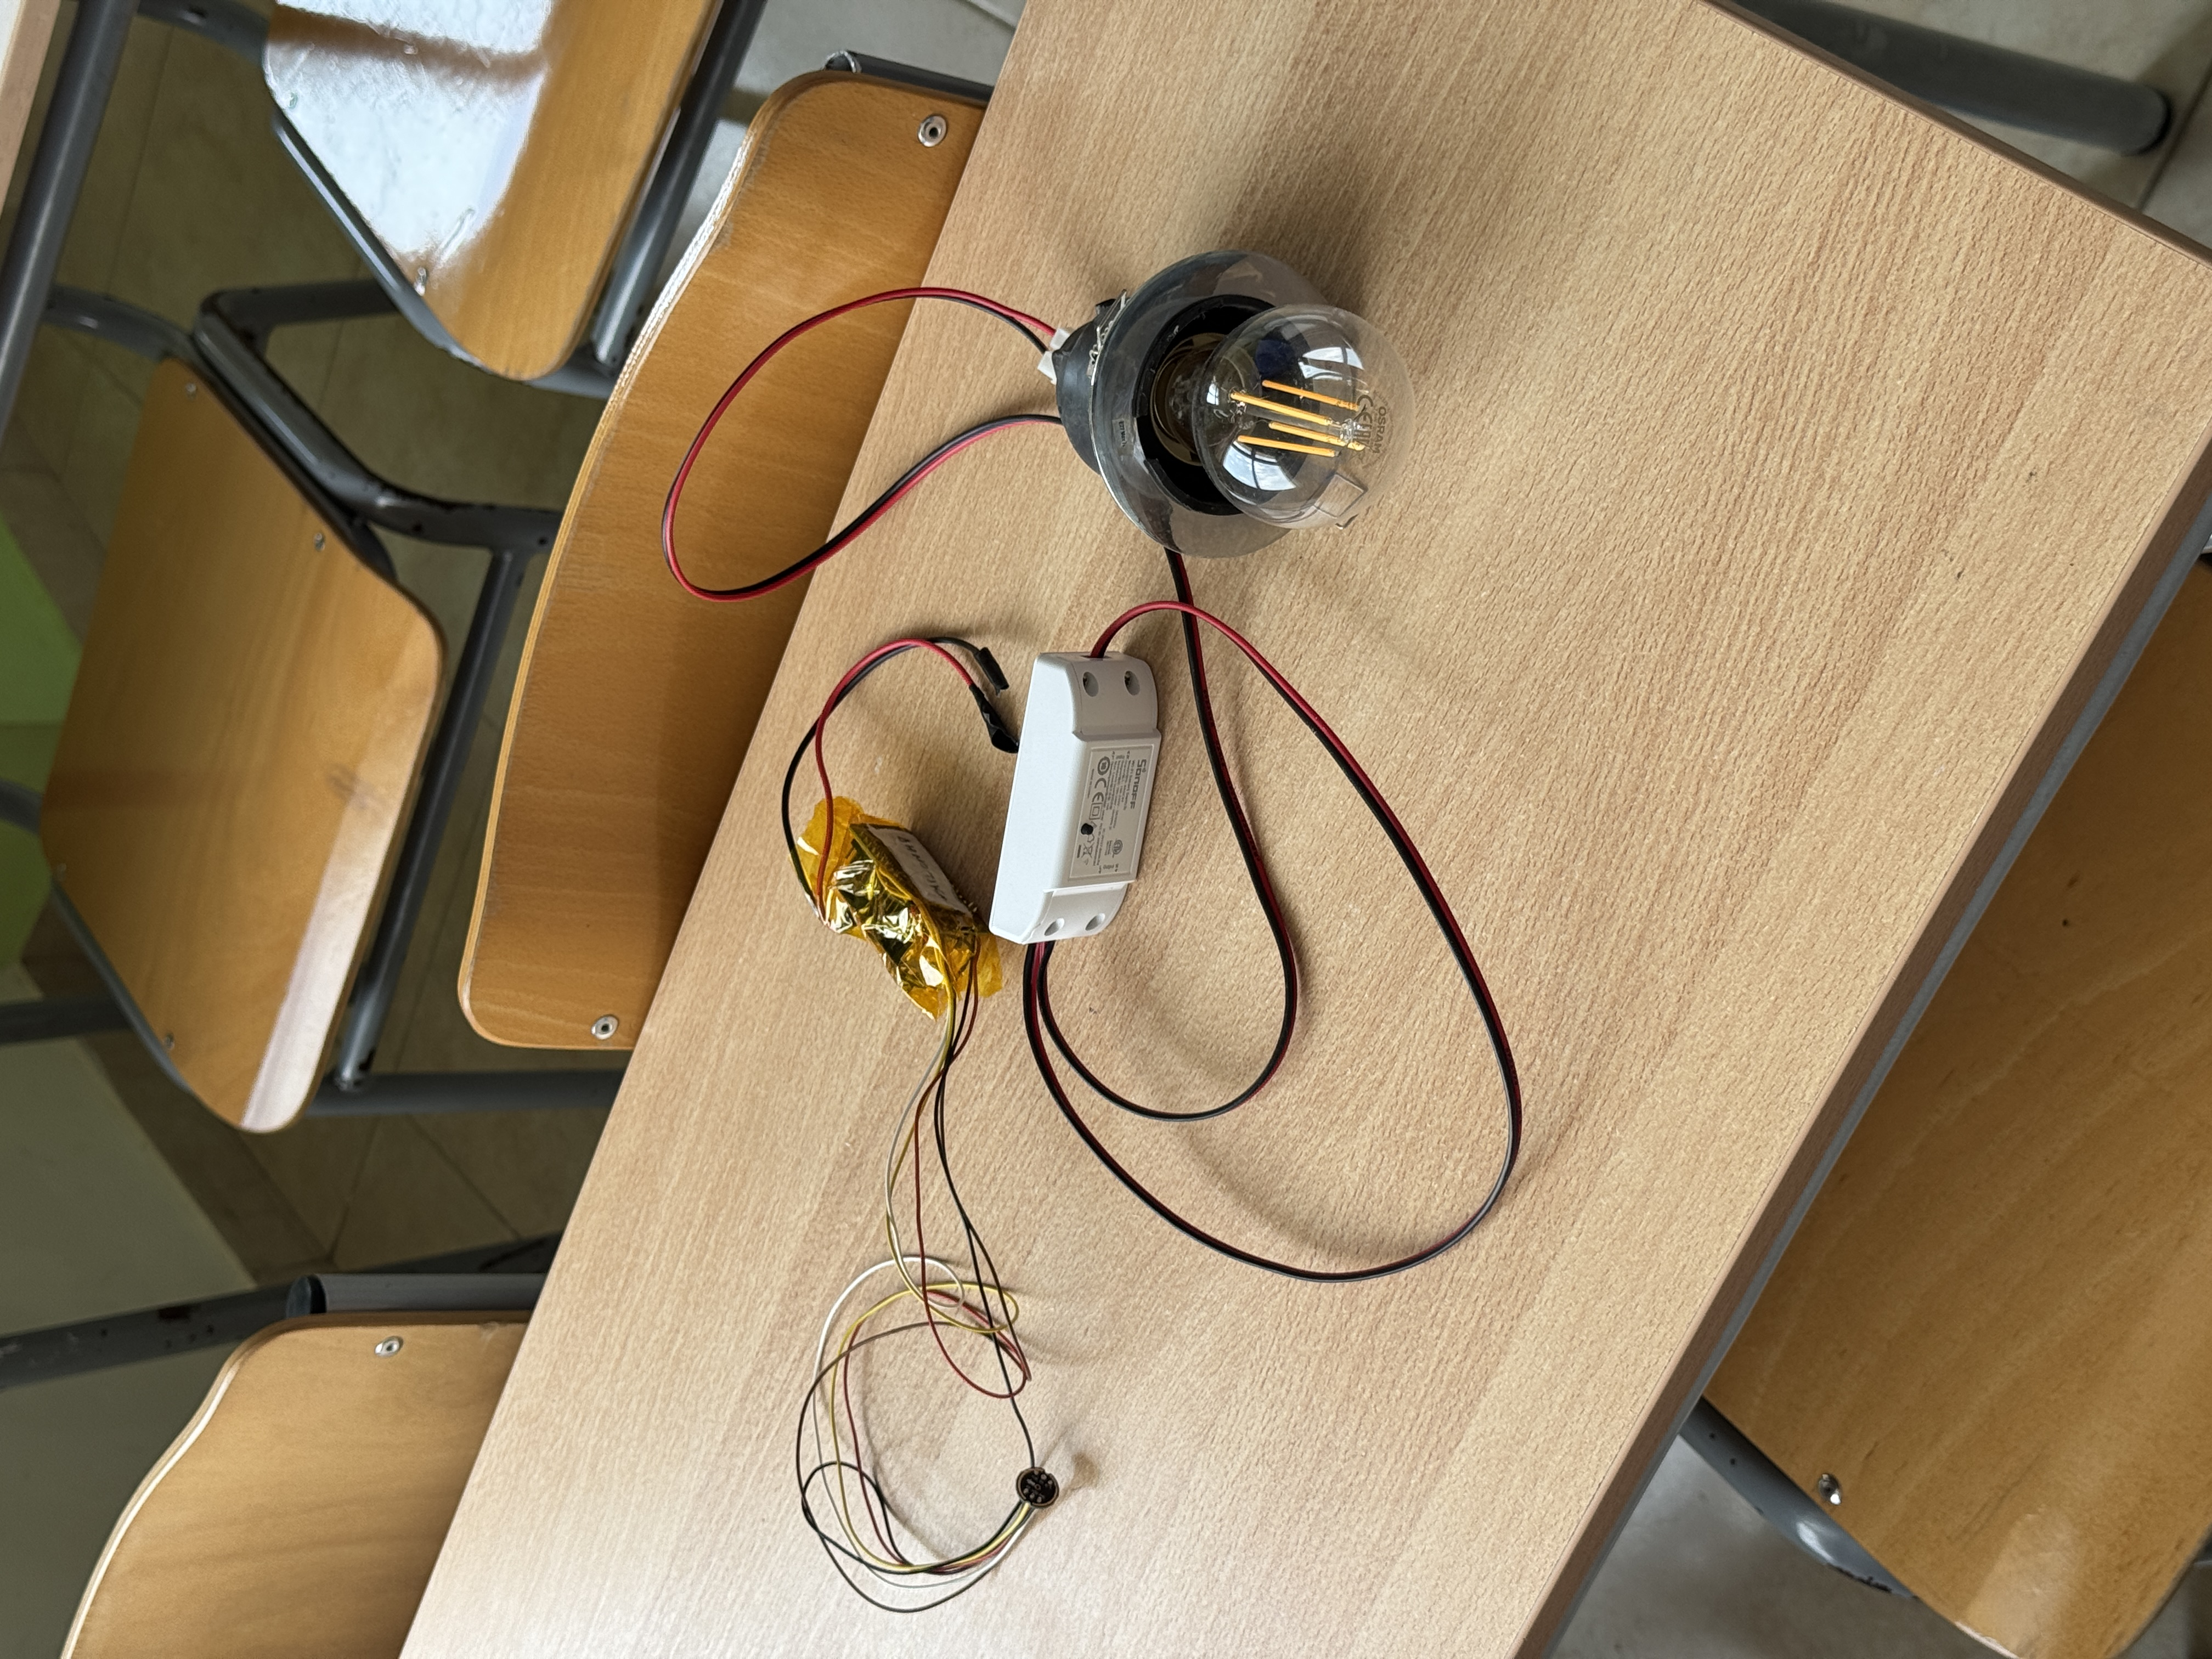
\includegraphics[angle=-90,width=0.31\textwidth]{fig_3_6}\hfill
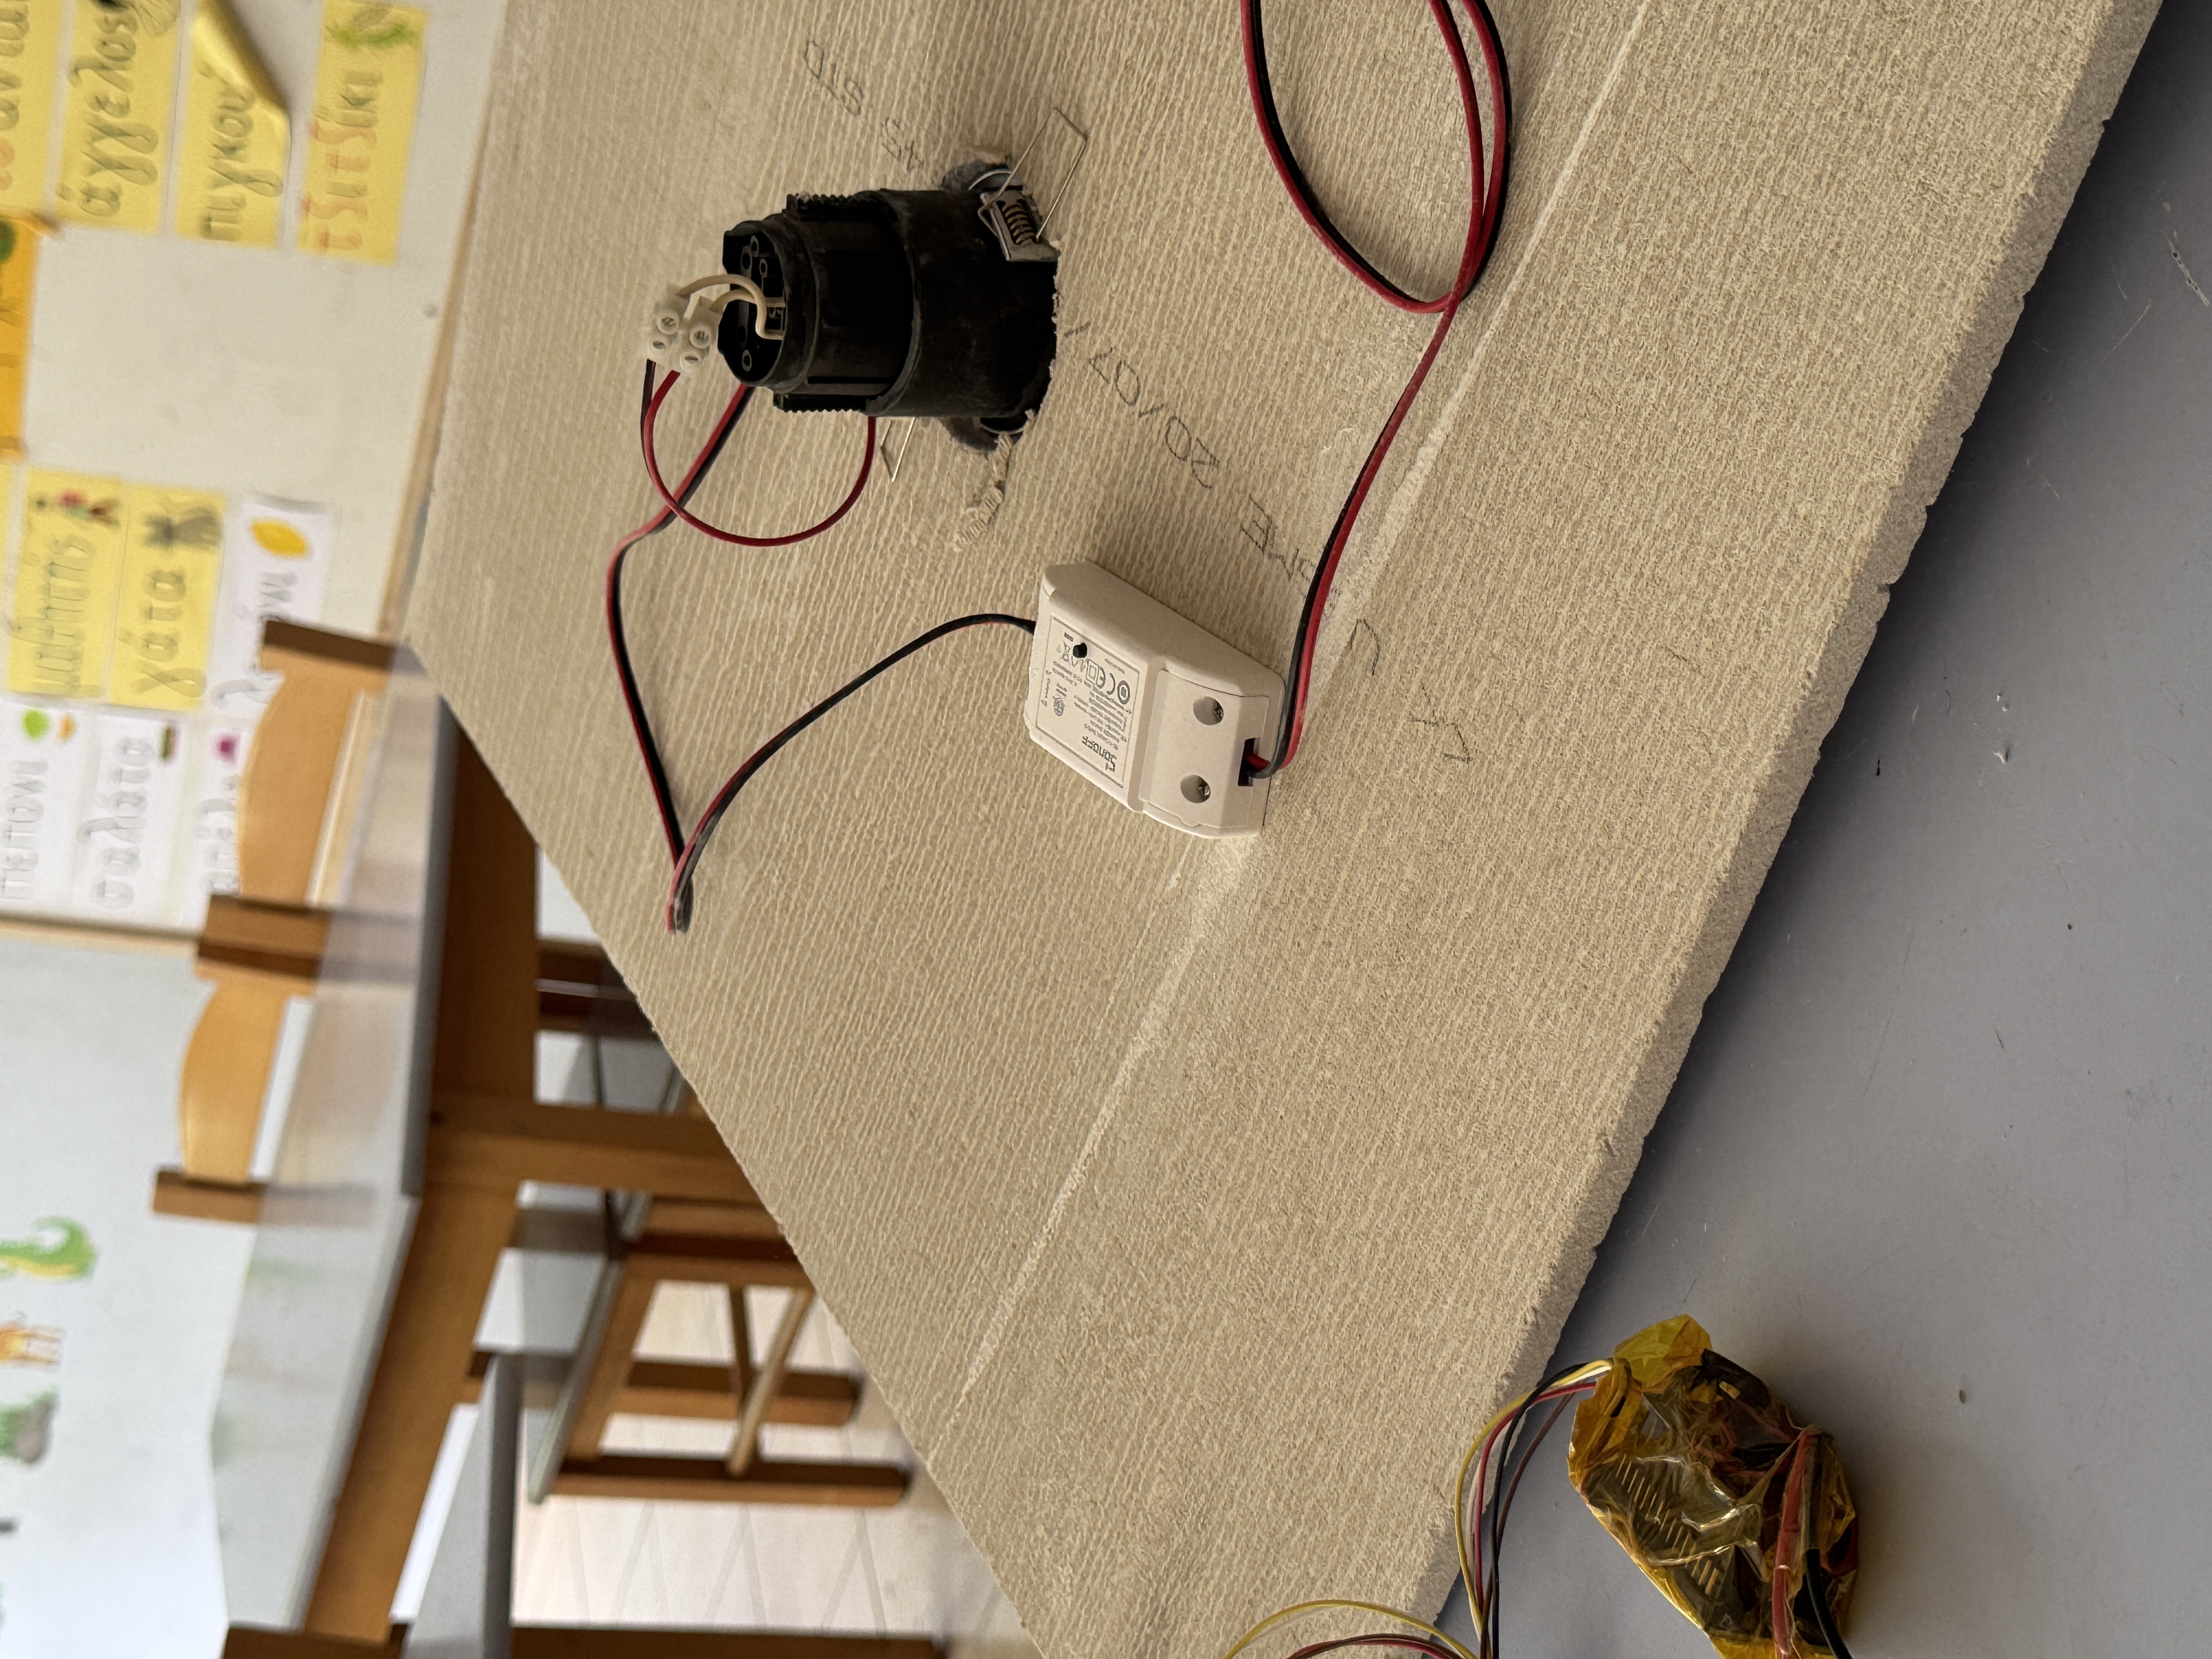
\includegraphics[angle=-90,width=0.31\textwidth]{fig_3_7}\hfill
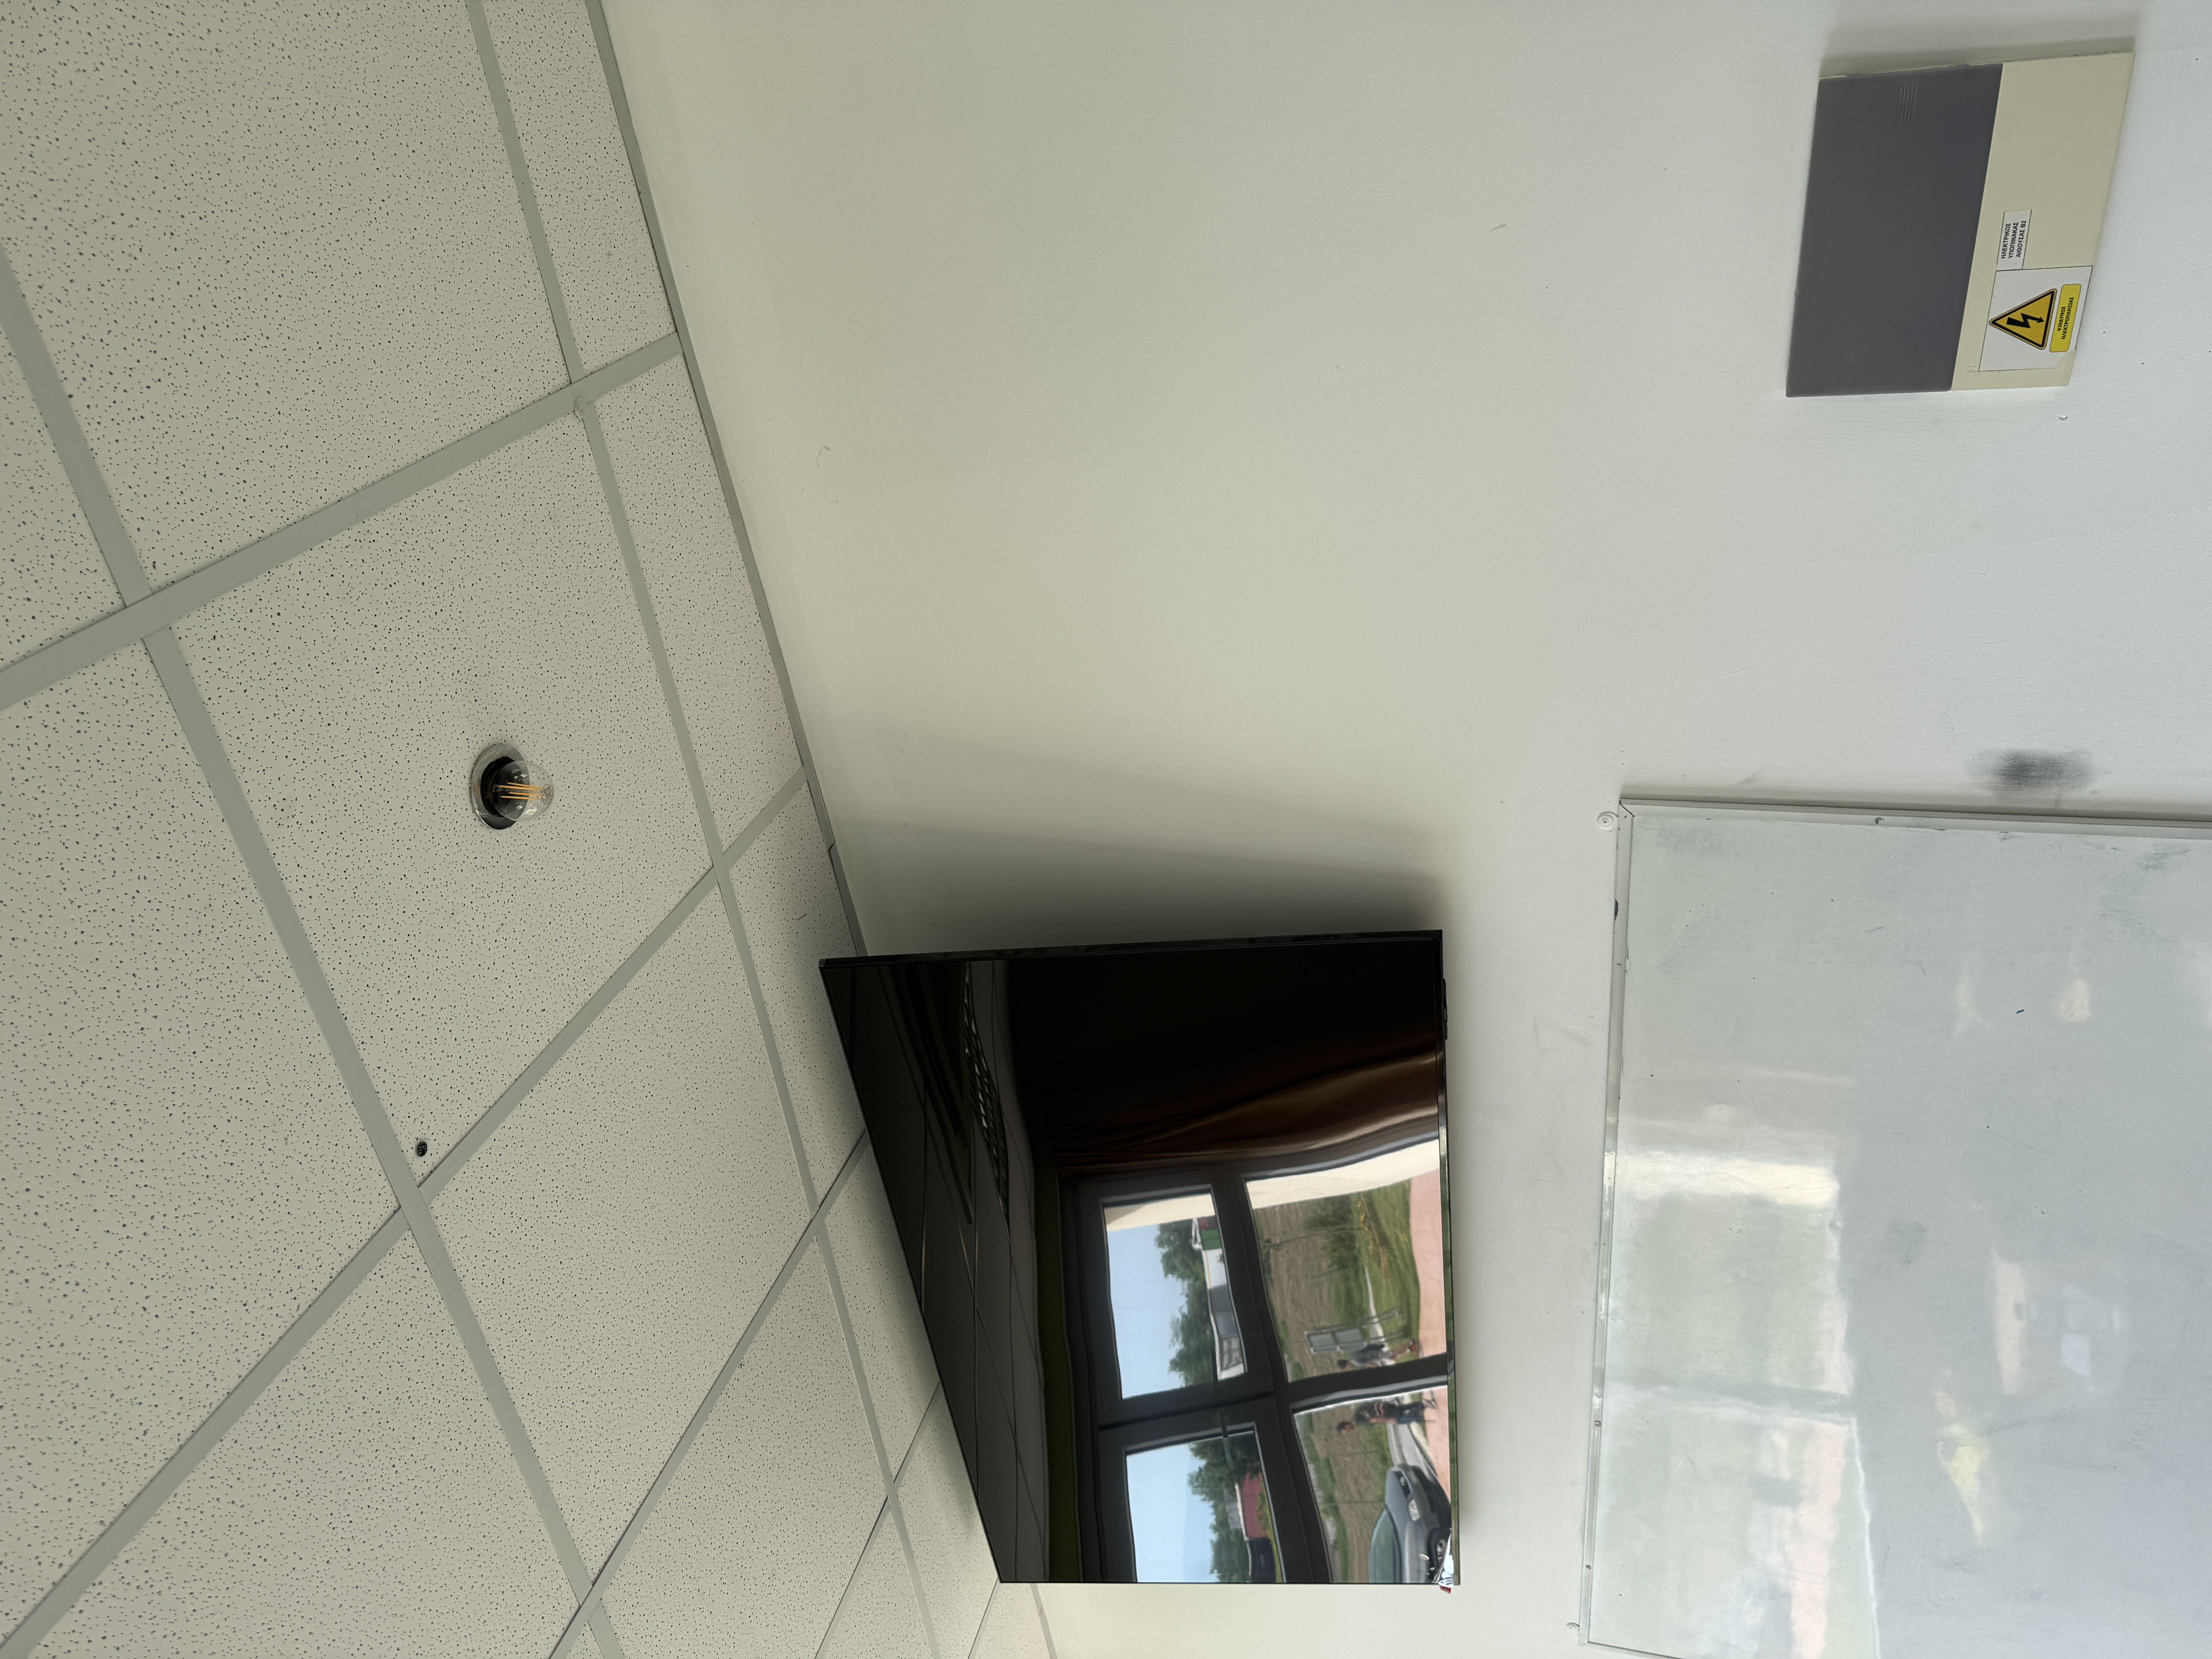
\includegraphics[angle=-90,width=0.31\textwidth]{fig_3_8}

\vspace{0.5em}

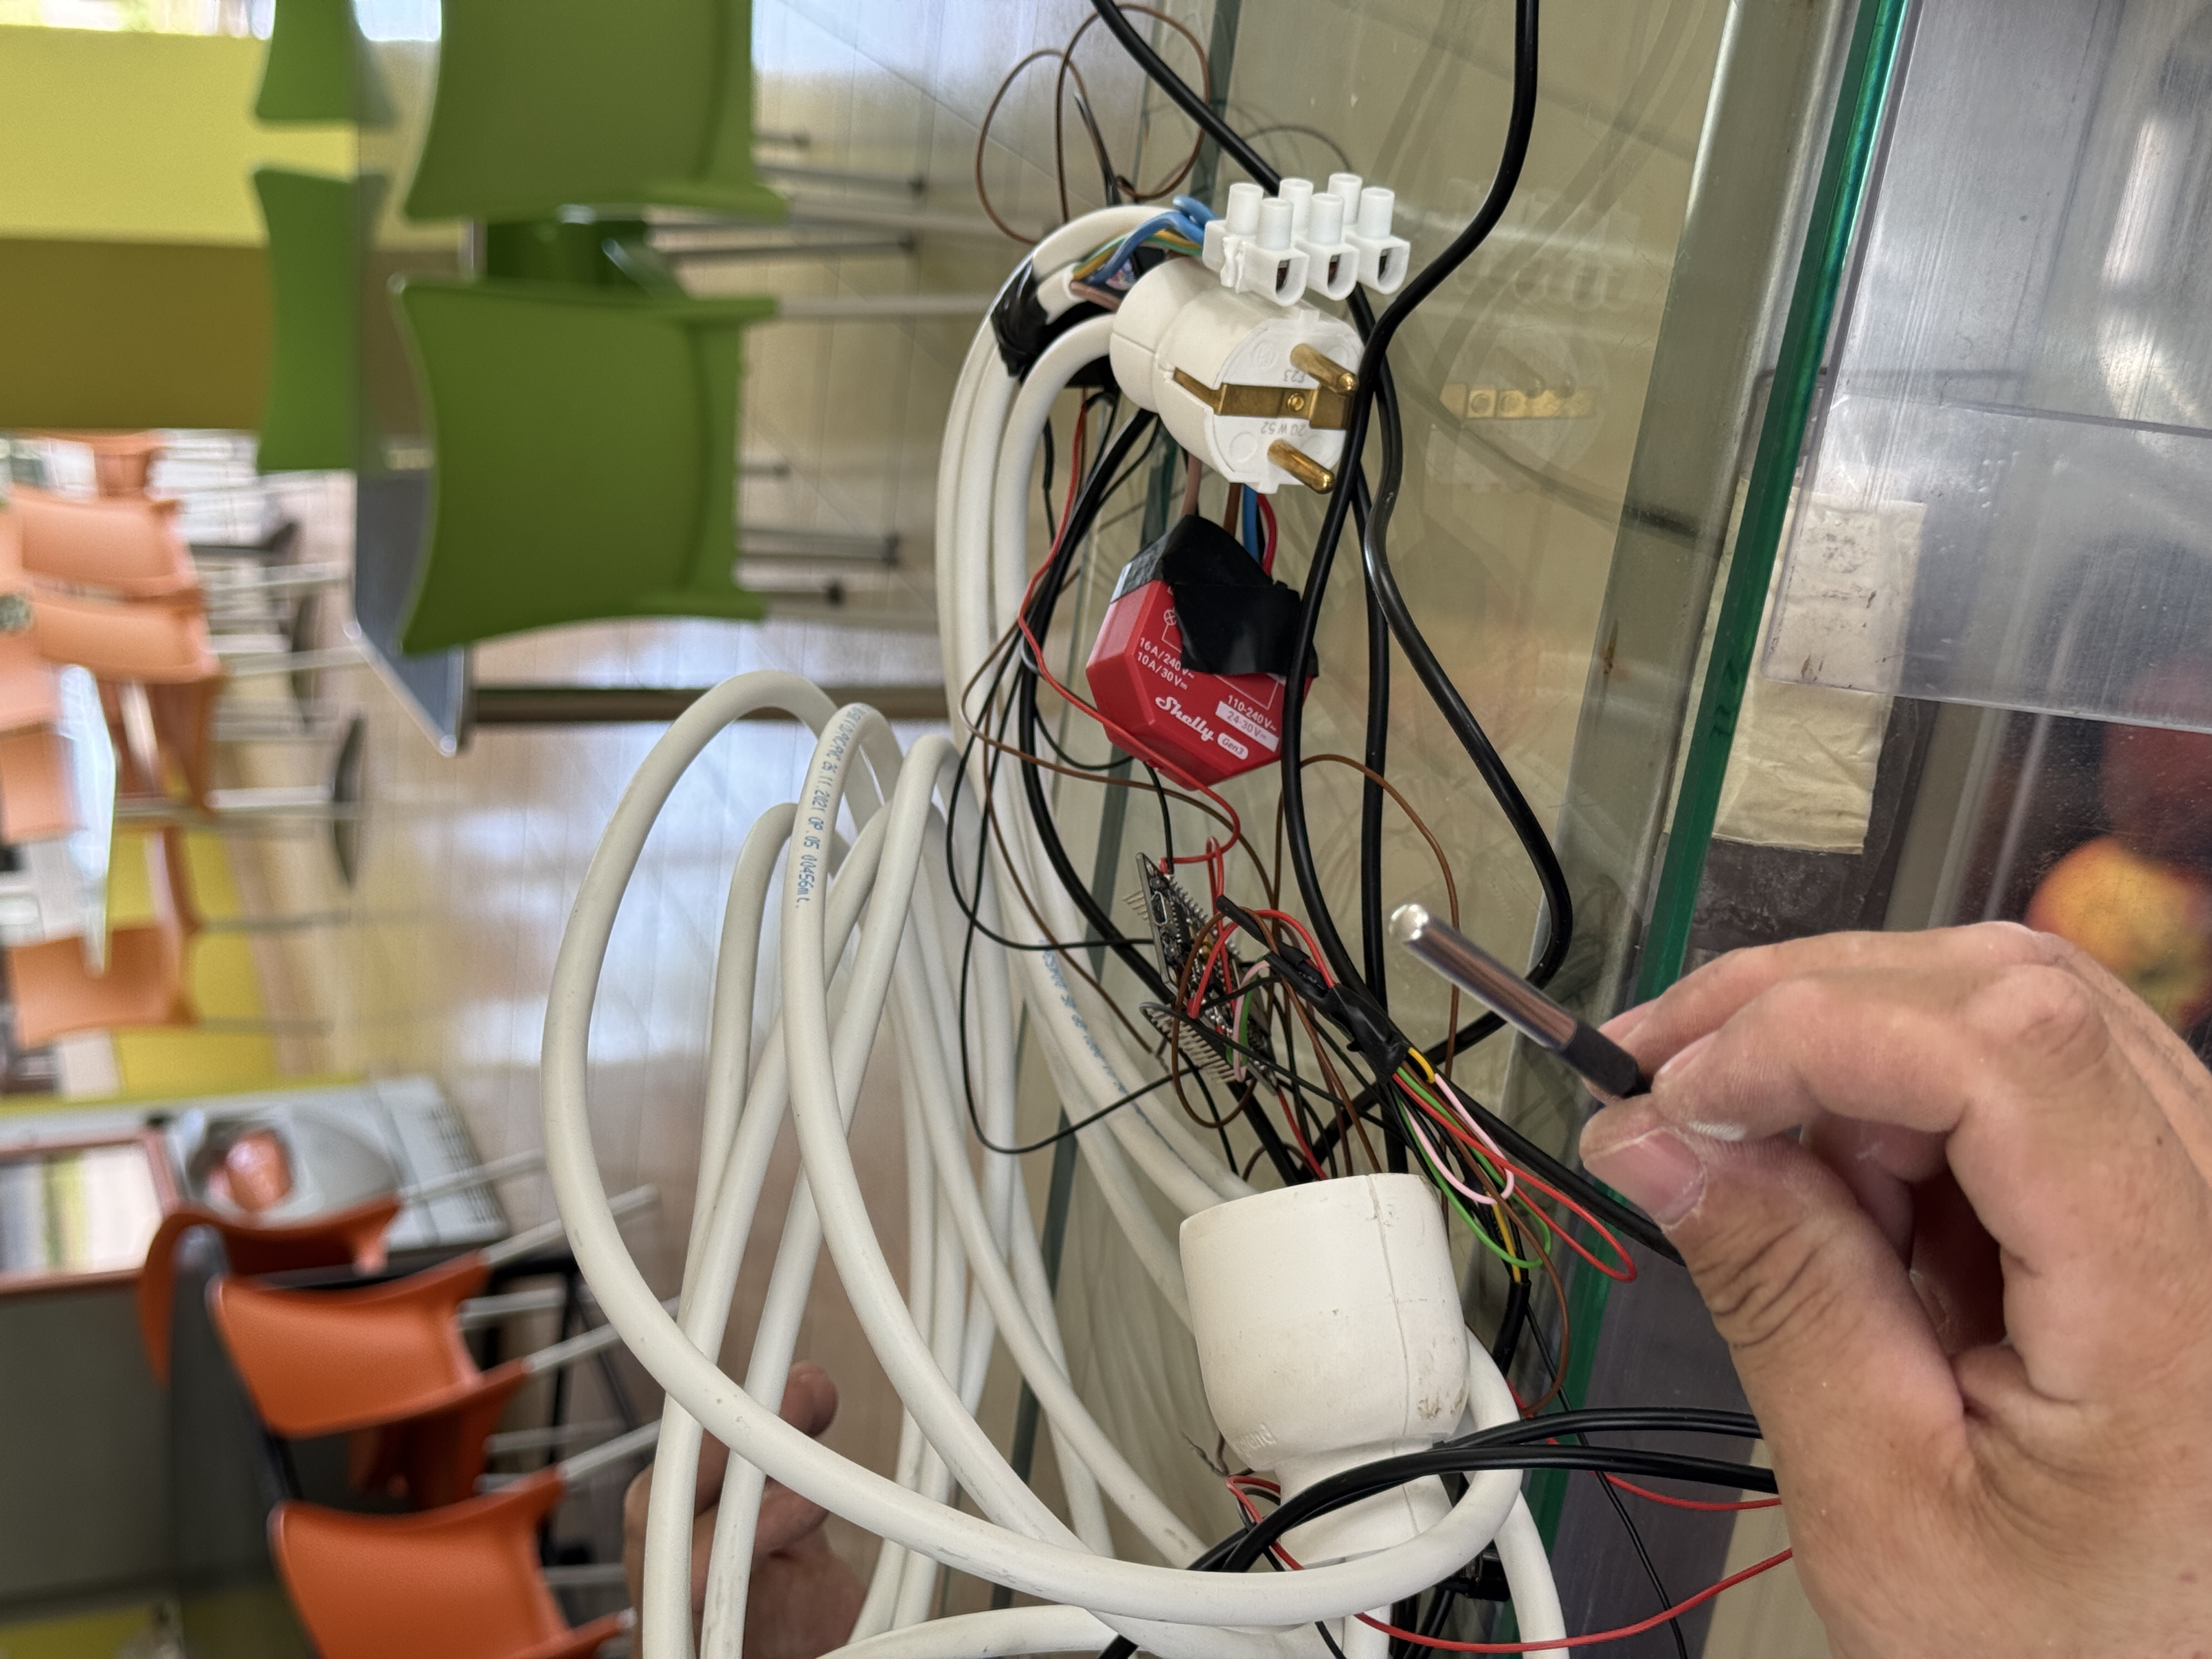
\includegraphics[angle=-90,width=0.31\textwidth]{fig_3_9}\hfill
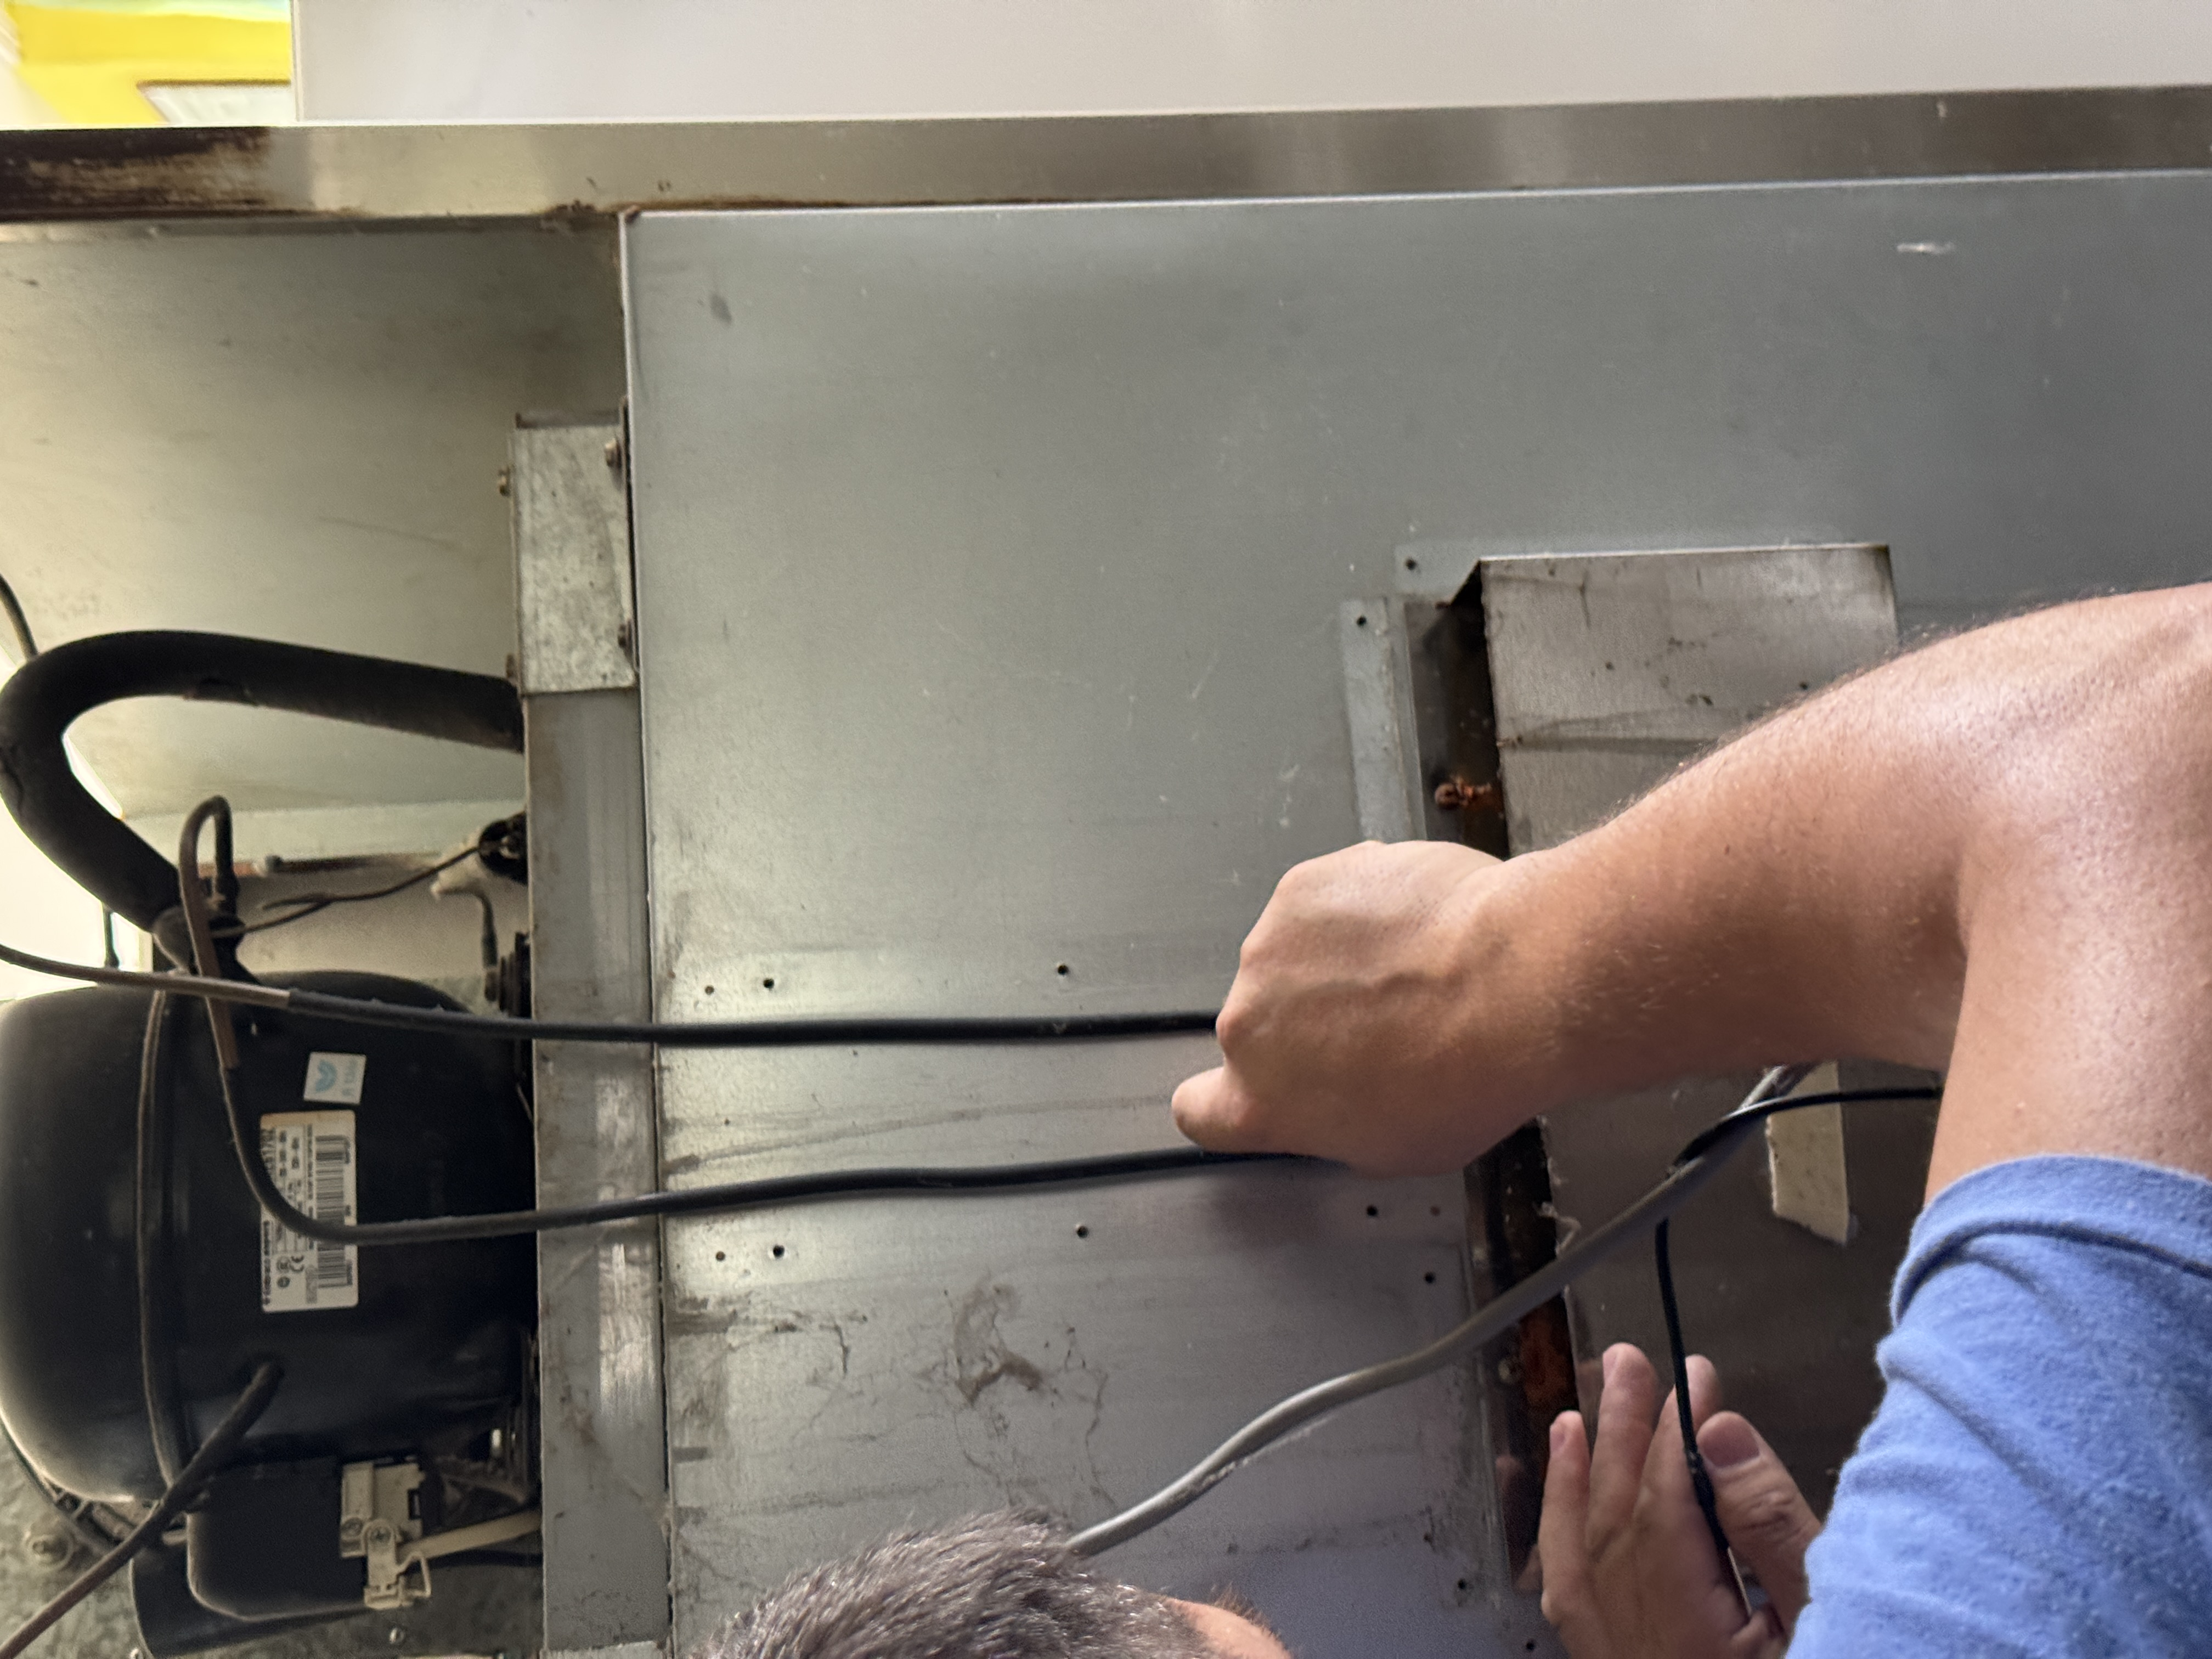
\includegraphics[angle=-90,width=0.31\textwidth]{fig_3_10}\hfill
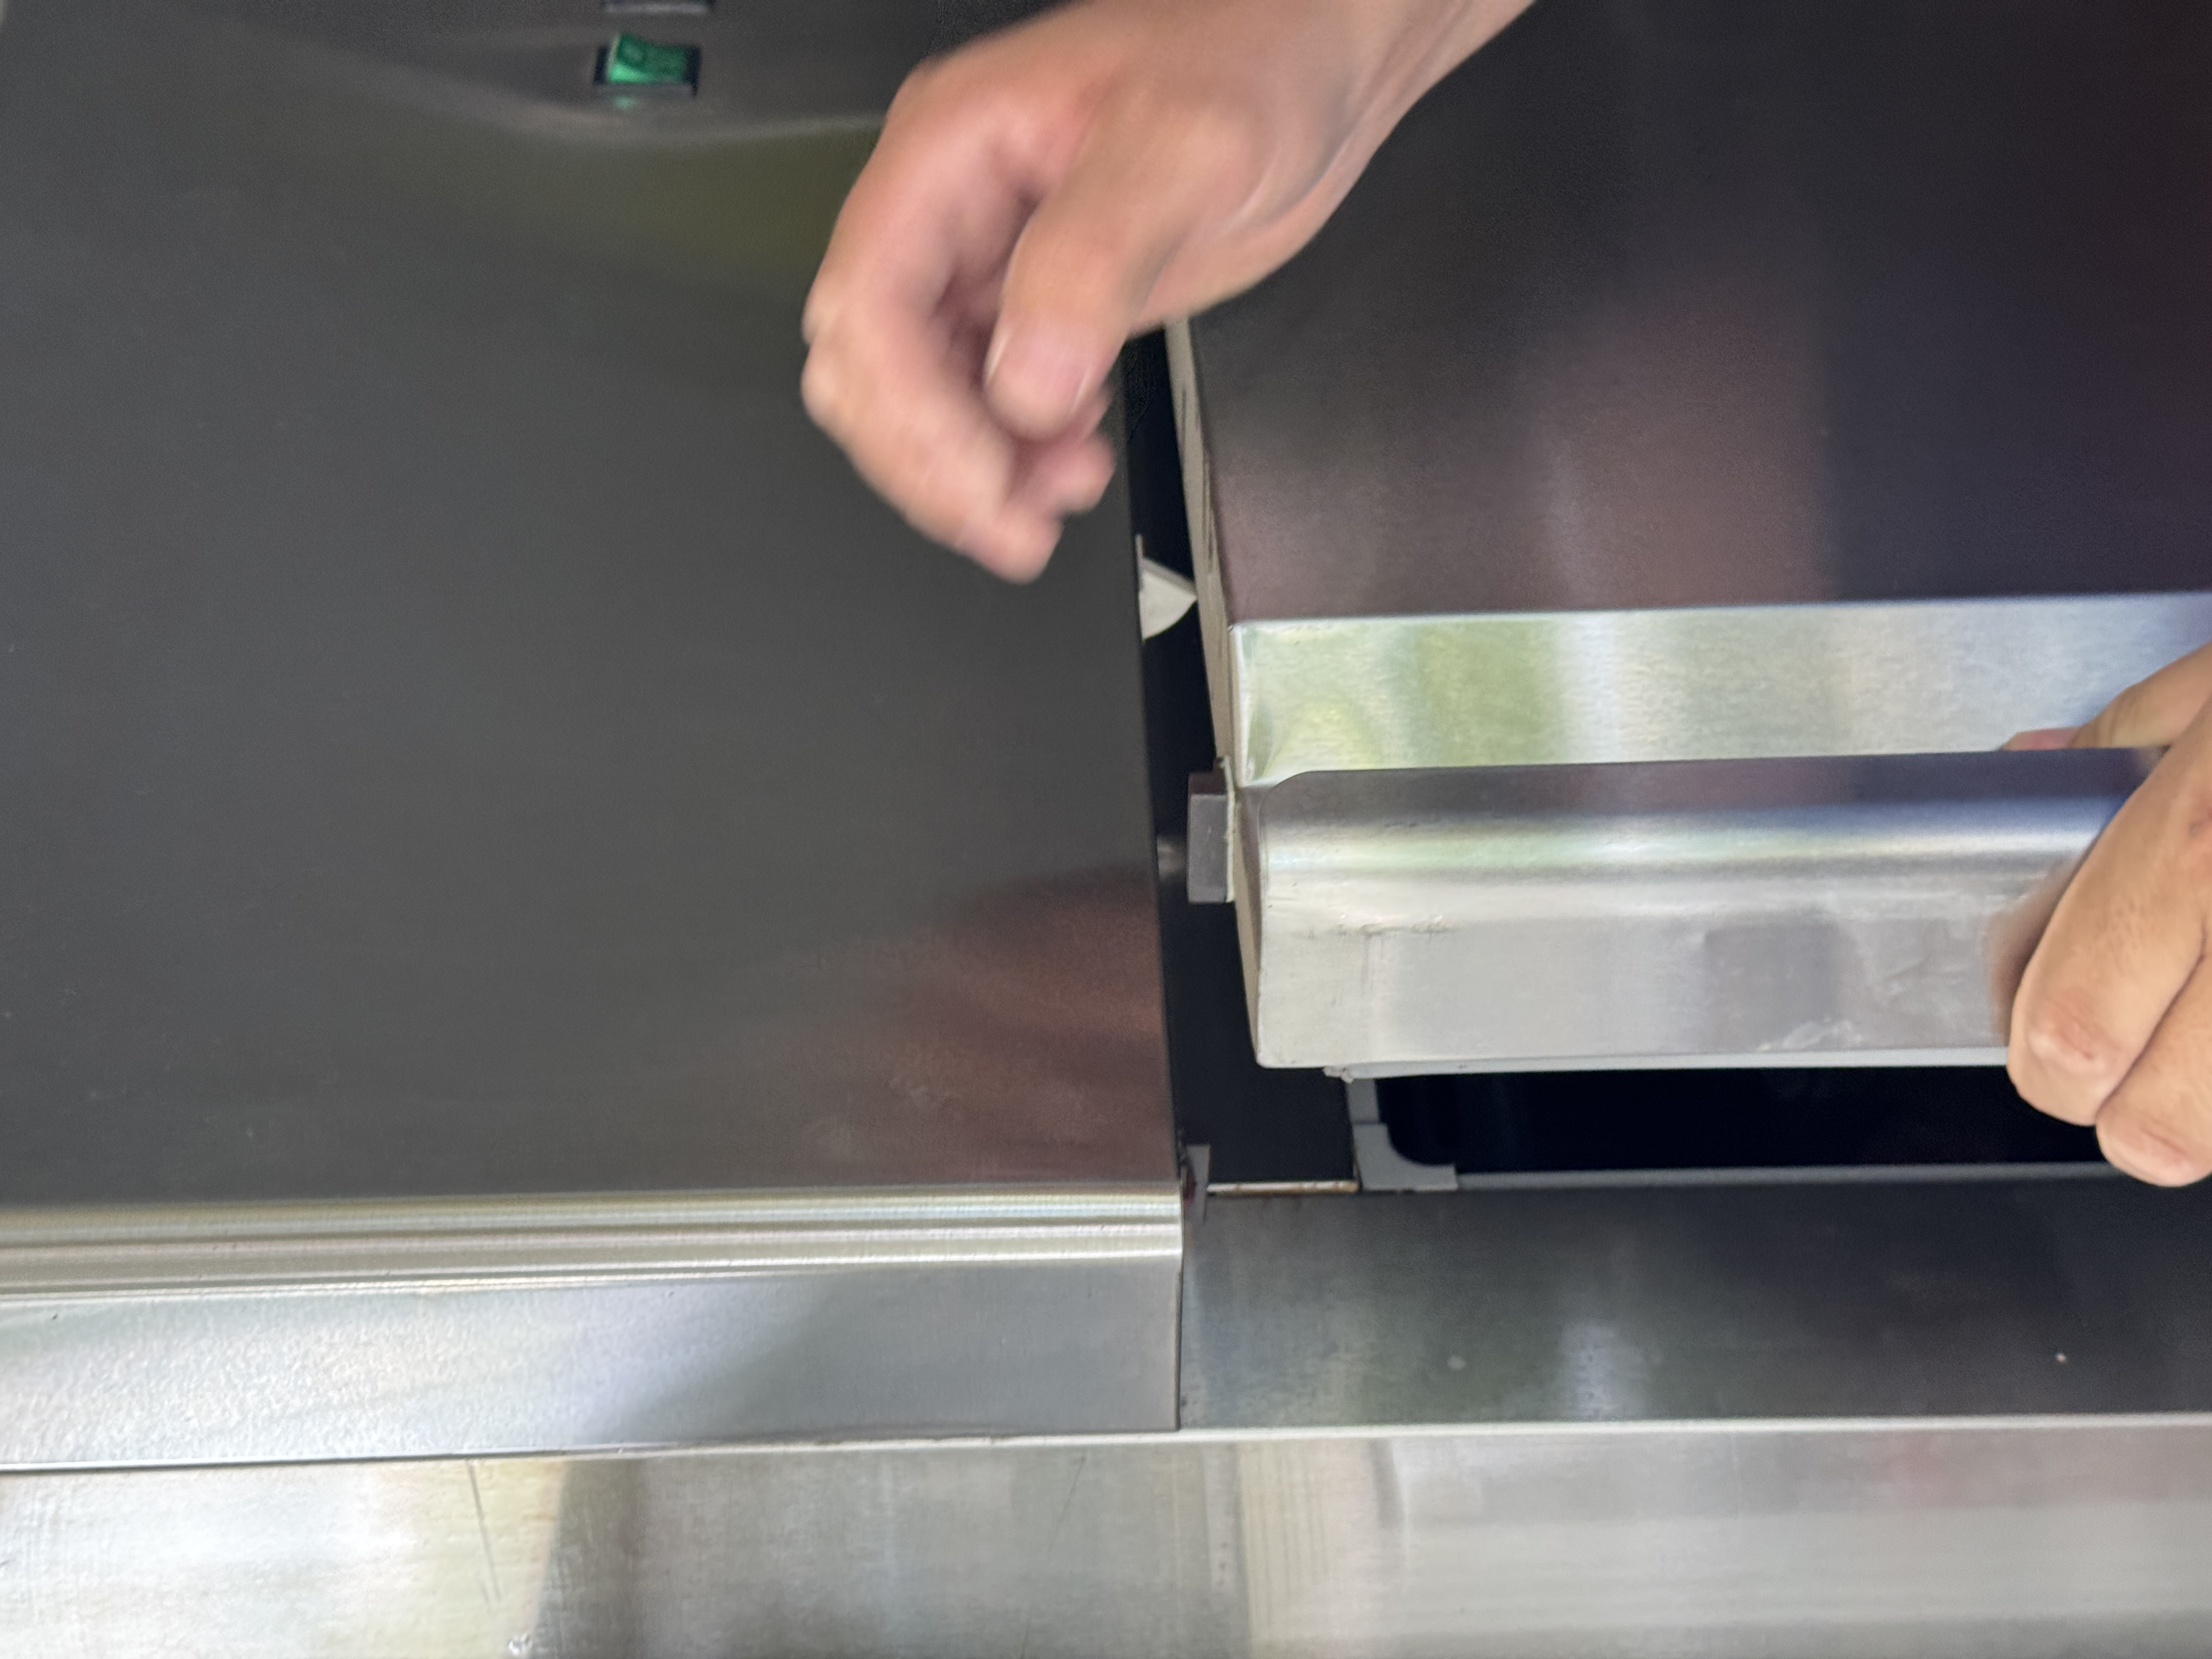
\includegraphics[angle=-90,width=0.31\textwidth]{fig_3_11}

\vspace{0.5em}

\caption{Φωτογραφίες από την εγκατάσταση στα Εκπαιδευτήρια Πλάτων. Πάνω σειρά: εγκατάσταση κόμβων ακουστικής παρακολούθησης και \textlatin{quiet-lamp} στις αίθουσες διδασκαλίας. Κάτω σειρά: εγκατάσταση αισθητήρων και έξυπνων μετρητών στον χώρο του κυλικείου.}
\label{fig:field_installation}
\end{figure}

\section{Η Αρχιτεκτονική των Πέντε Επιπέδων}
Η αρχιτεκτονική της πλατφόρμας υιοθετεί και προσαρμόζει το θεωρητικό μοντέλο πέντε επιπέδων της βιβλιογραφίας στις απαιτήσεις του σχολικού περιβάλλοντος, όπως αποτυπώνεται στο Σχήμα~\ref{fig:five_layer_architecture}. Τα επίπεδα \textlatin{Physical} και \textlatin{Connection} παραμένουν ως έχουν, ενώ τα επίπεδα \textlatin{Data}, \textlatin{Virtual} και \textlatin{Service} προσαρμόζονται σε \textlatin{Edge Middleware}, \textlatin{Cloud Data and Services} και \textlatin{Application and UX} αντίστοιχα --- αντικατοπτρίζοντας την πραγματική τεχνολογική στοίβα της υλοποίησης.

\begin{figure}[htbp]
\centering
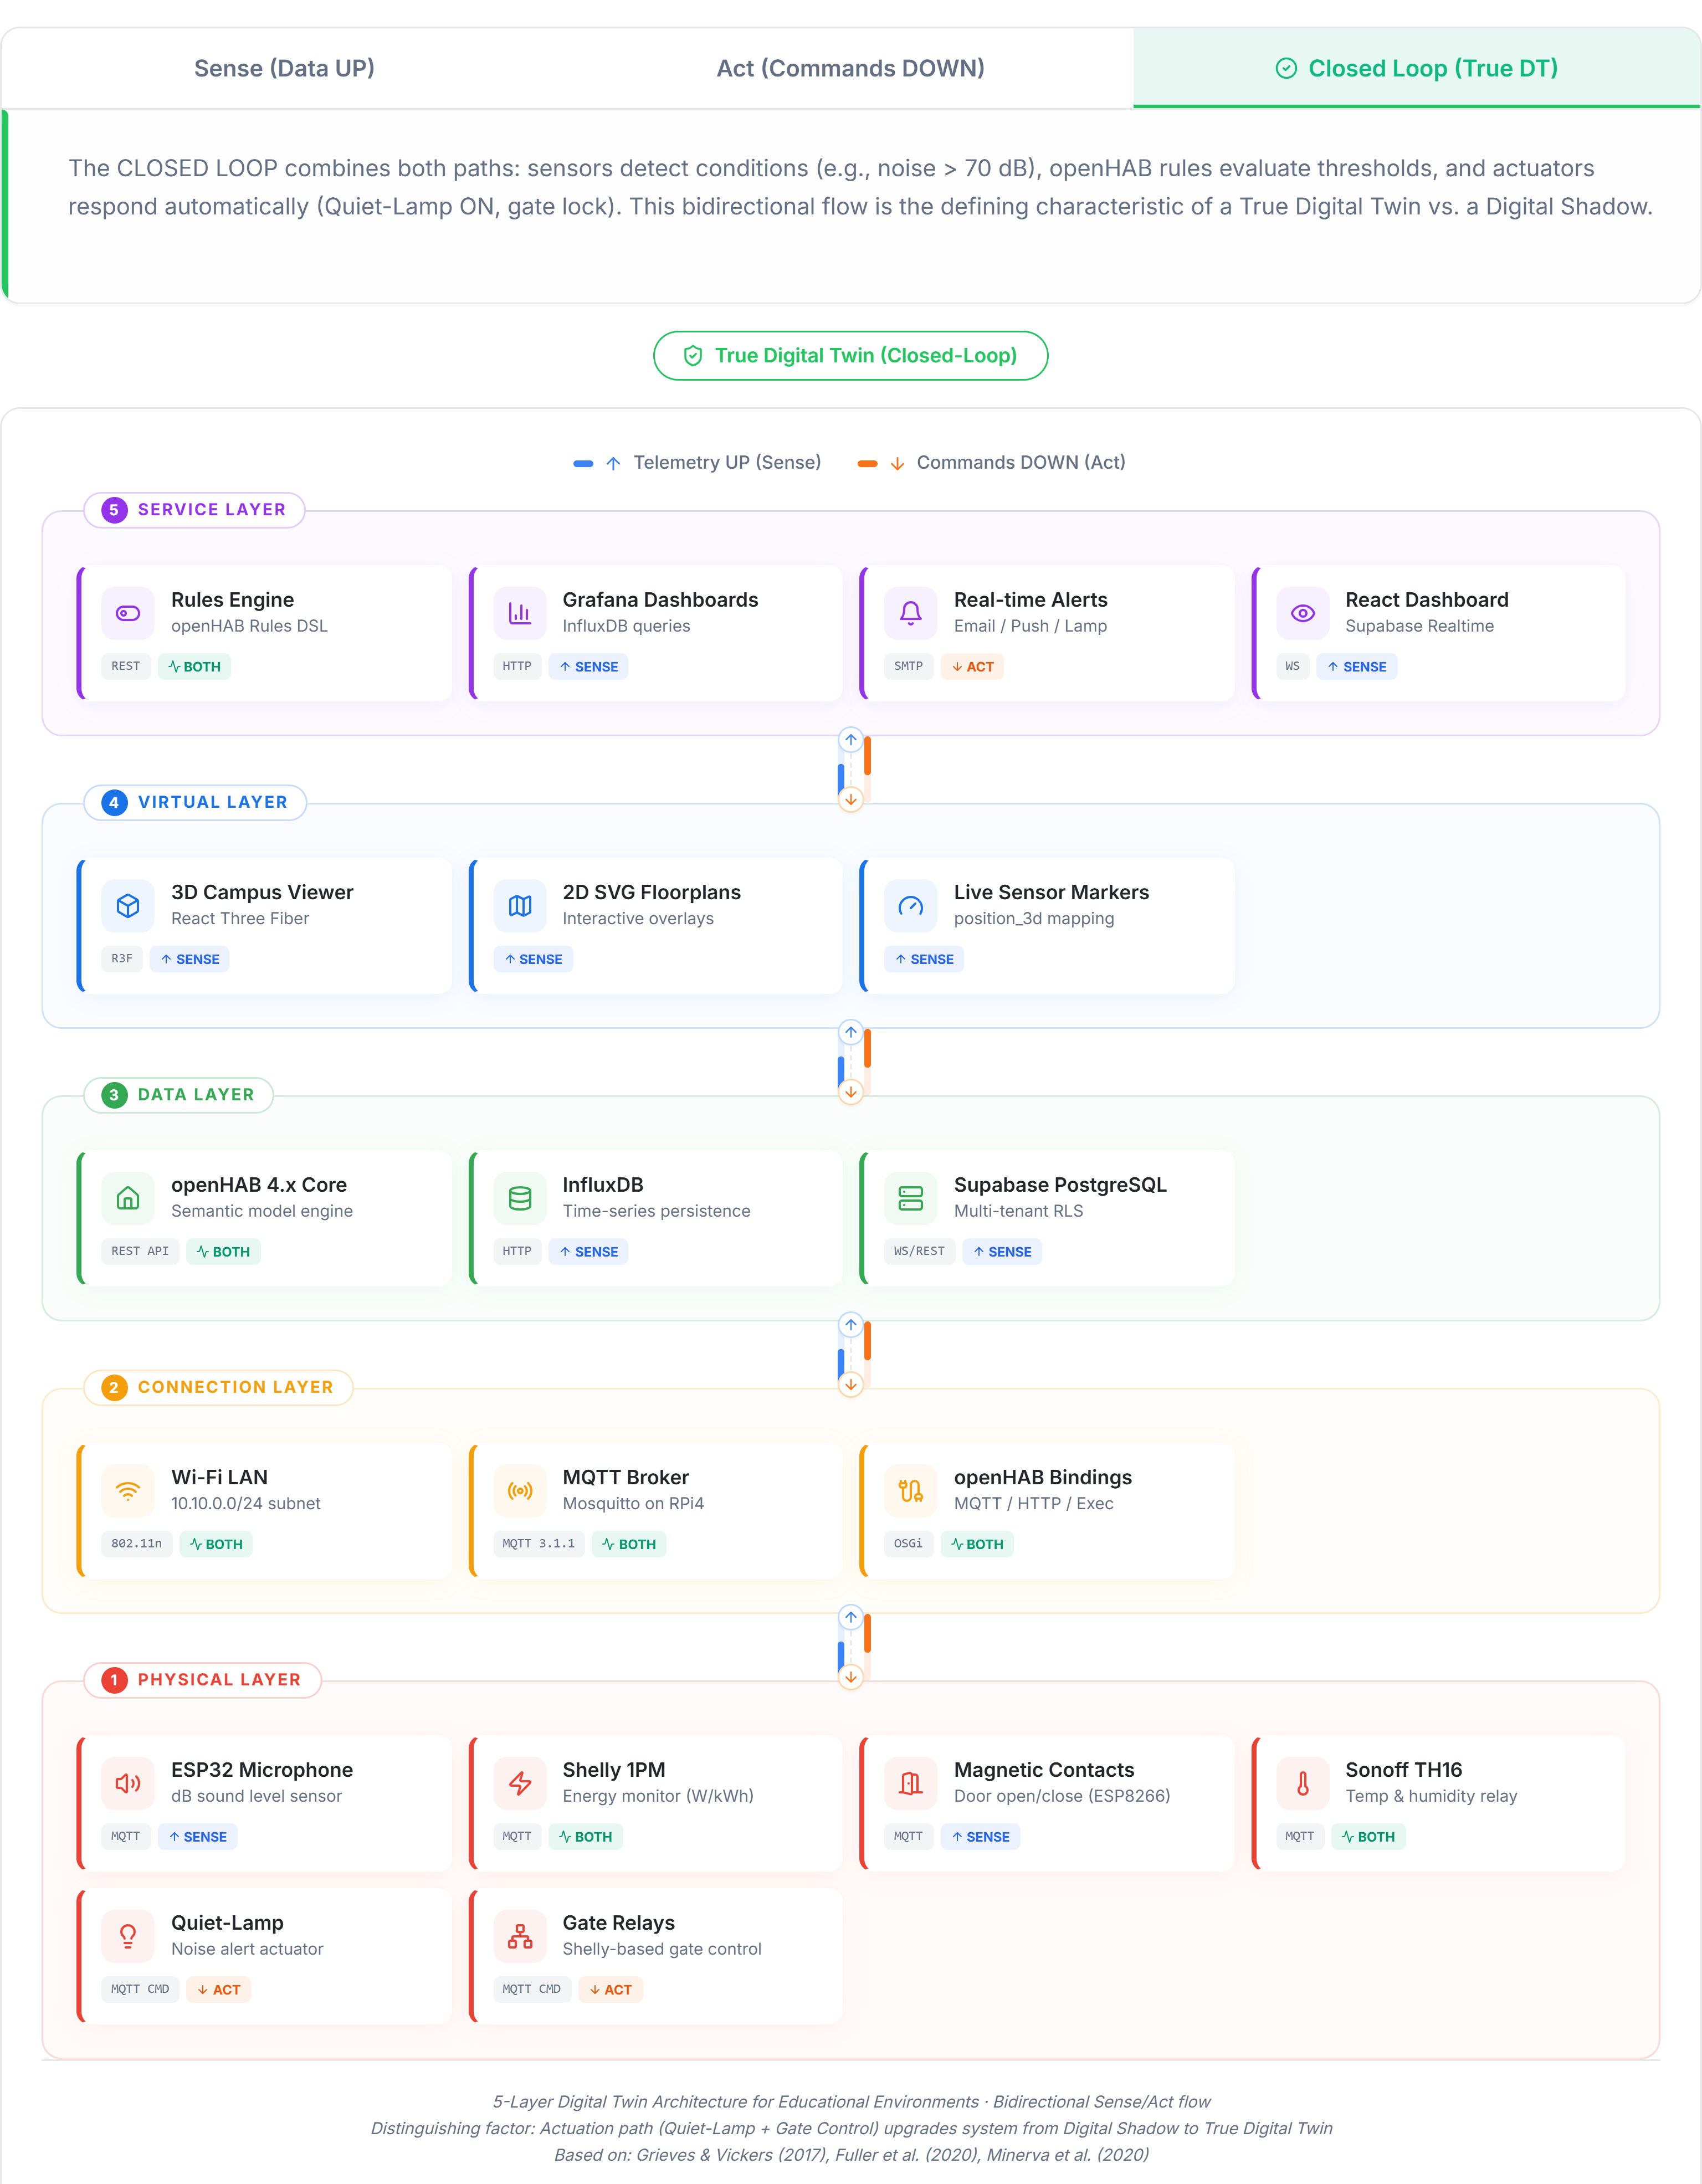
\includegraphics[width=\textwidth]{fig_3_1}
\caption{Συνοπτική απεικόνιση της αρχιτεκτονικής πέντε επιπέδων της πλατφόρμας Ψηφιακού Διδύμου.}
\label{fig:five_layer_architecture}
\end{figure}

\subsection{\texorpdfstring{\textlatin{Physical Layer}}{Physical Layer}}
Το \textlatin{Physical Layer} περιλαμβάνει το σύνολο του υλικού εξοπλισμού της εγκατάστασης: τους κόμβους \textlatin{ESP32/INMP441} για μέτρηση ακουστικής στάθμης στις αίθουσες, τον μετρητή ισχύος \textlatin{Shelly 1PM Mini Gen3} για παρακολούθηση κατανάλωσης ψυγείου, τον κόμβο \textlatin{ESP8266} με μαγνητική επαφή \textlatin{MC-38} για ανίχνευση ανοίγματος θύρας, τα ρελέ \textlatin{Sonoff Basic R2} για έλεγχο \textlatin{quiet-lamp} και \textlatin{buzzer}, και τις \textlatin{dry-contact} επαφές ενοποίησης με τον υπάρχοντα ελεγκτή των αυτόματων πυλών. Όλες οι συσκευές επικοινωνούν ασύρματα μέσω \textlatin{WiFi} με το επόμενο επίπεδο.

\subsection{\texorpdfstring{\textlatin{Connection Layer}}{Connection Layer}}
Το \textlatin{Connection Layer} αναλαμβάνει τη μεταφορά δεδομένων μεταξύ φυσικών συσκευών και λογισμικού. Ο \textlatin{MQTT broker} \textlatin{Mosquitto} εκτελείται στον \textlatin{Raspberry Pi 4} και δέχεται \textlatin{telemetry} από όλους τους κόμβους. Τα \textlatin{openHAB Bindings} (\textlatin{MQTT Binding}, \textlatin{HTTP Binding}) μεταφράζουν τα μηνύματα σε \textlatin{openHAB Items}, δημιουργώντας ενιαία αναπαράσταση ανεξάρτητα από το πρωτόκολλο κάθε συσκευής.

\subsection{\texorpdfstring{\textlatin{Edge Middleware Layer}}{Edge Middleware Layer}}
Το \textlatin{Edge Middleware Layer} αποτελεί τον εγκέφαλο της τοπικής υποδομής και εκτελείται εξ ολοκλήρου στον \textlatin{Raspberry Pi 4}. Το \textlatin{openHAB 4.x Core} με το \textlatin{Semantic Model} (\textlatin{Location}$\rightarrow$\textlatin{Building}$\rightarrow$\textlatin{Floor}$\rightarrow$\textlatin{Room}$\rightarrow$\textlatin{Equipment}$\rightarrow$\textlatin{Point} ιεραρχία) οργανώνει σημασιολογικά όλες τις συσκευές της εγκατάστασης. Ο \textlatin{Rules Engine} υλοποιεί τη λογική αυτοματισμού --- τον κανόνα \textlatin{NoiseGuard} για ακουστική παρέμβαση και τον κανόνα \textlatin{FridgeGuardian} για παρακολούθηση ψυγείου --- κλείνοντας τον βρόχο ελέγχου από το \textlatin{Sense} στο \textlatin{Act}. Η \textlatin{InfluxDB} αποθηκεύει χρονοσειρές τηλεμετρίας για ιστορική ανάλυση.

\subsection{\texorpdfstring{\textlatin{Cloud Data and Services Layer}}{Cloud Data and Services Layer}}
Το \textlatin{Cloud Data and Services Layer} παρέχει την απομακρυσμένη αποθήκευση και τις υπηρεσίες \textlatin{backend} της πλατφόρμας. Η \textlatin{Supabase PostgreSQL} αποθηκεύει τη διαμόρφωση της πλατφόρμας, τα δεδομένα χρηστών και το ιστορικό διαμόρφωσης και \textlatin{installation metadata}. Οι \textlatin{Supabase Edge Functions} παρέχουν \textlatin{REST API} για επικοινωνία με το \textlatin{frontend} και ενσωμάτωση με το \textlatin{Gemini API} για \textlatin{LLM-based energy forecasting}. Το σύστημα \textlatin{real-time alerts} αποστέλλει αυτόματες ειδοποιήσεις σε ανωμαλίες που εντοπίζει ο \textlatin{Rules Engine}.

\subsection{\texorpdfstring{\textlatin{Application and UX Layer}}{Application and UX Layer}}
Το \textlatin{Application and UX Layer} παρέχει την τελική διεπαφή προς τον χρήστη μέσω της \textlatin{Cloud SaaS} πλατφόρμας που είναι προσβάσιμη στη διεύθυνση \textlatin{digitaltwin.pi-tech.gr}. Το \textlatin{React 18 dashboard} προσφέρει \textlatin{3D campus visualization} μέσω \textlatin{React Three Fiber}, \textlatin{2D SVG floor plans} με κατάσταση αιθουσών, \textlatin{real-time} παρακολούθηση αισθητήρων και αμφίδρομο έλεγχο συσκευών. Η πρόσβαση διέπεται από \textlatin{RBAC} πολυεπίπεδης εξουσιοδότησης με ξεχωριστούς ρόλους για διαχειριστή και χρήστη.

\section{Σημασιολογική Οργάνωση και Διαλειτουργικότητα}
Η παρούσα πλατφόρμα σχεδιάστηκε με έμφαση στη διαλειτουργικότητα, ώστε να μην περιορίζεται σε νέες συσκευές \textlatin{IoT}, αλλά να μπορεί να ενοποιεί και υφιστάμενες εγκαταστάσεις του σχολείου. Χαρακτηριστικό παράδειγμα αποτελεί η διασύνδεση με το ήδη εγκατεστημένο σύστημα αυτόματων πυλών, το οποίο εντάχθηκε στο ενιαίο περιβάλλον ελέγχου χωρίς αντικατάσταση του φυσικού εξοπλισμού, αλλά μέσω λογισμικής διασύνδεσης και κοινής διαχείρισης κατάστασης.

Η επιλογή αυτή ακολουθεί τη λογική του \textlatin{Brownfield Integration}: αντί για εκ βάθρων ανακατασκευή της υποδομής, η πλατφόρμα λειτουργεί ως επίπεδο ενοποίησης ανάμεσα σε ετερογενή υποσυστήματα, επιτρέποντας κοινή εποπτεία, ενοποιημένους κανόνες ελέγχου και σταδιακή επέκταση σε νέα σημεία του σχολείου. Από τεχνική άποψη, η προσέγγιση αυτή μειώνει το κόστος μετάβασης, περιορίζει την εξάρτηση από ιδιόκτητα συστήματα και καθιστά ρεαλιστική την υιοθέτηση του \textlatin{Digital Twin} σε υφιστάμενα σχολικά κτίρια.





\chapter{Τεχνική Υλοποίηση Συστήματος}
Το παρόν κεφάλαιο αναλύει την τεχνική υλοποίηση του ψηφιακού διδύμου, παρουσιάζοντας το σύστημα όχι ως στατική κατασκευή, αλλά ως αποτέλεσμα μιας εξελικτικής πορείας δύο διακριτών φάσεων. Η πρώτη φάση αντιστοιχεί στο τοπικό πρωτότυπο (\textlatin{Proof of Concept} ή \textlatin{MVP}), μέσω του οποίου επιβεβαιώθηκε η αξιοπιστία της συλλογής δεδομένων, η λειτουργία των βασικών αυτοματισμών και η δυνατότητα \textlatin{closed-loop} ελέγχου. Η δεύτερη φάση αντιστοιχεί στην ωρίμανση του συστήματος προς μια πλήρως προσαρμοσμένη πλατφόρμα \textlatin{Enterprise Cloud SaaS}, η οποία μεταφέρει το επίκεντρο από το \textlatin{engineering console} περιβάλλον σε ένα \textlatin{user-centric}, \textlatin{cloud-native} και \textlatin{responsive} οικοσύστημα.

Η δομή του κεφαλαίου ακολουθεί αυτή ακριβώς τη λογική. Αρχικά περιγράφεται η τοπική υλοποίηση που στηρίχθηκε σε \textlatin{MQTT}, \textlatin{openHAB}, \textlatin{InfluxDB} και \textlatin{Grafana}. Στη συνέχεια παρουσιάζεται η νέα \textlatin{cloud-based} αρχιτεκτονική, με \textlatin{frontend} σε \textlatin{React 18} και \textlatin{backend} σε \textlatin{Supabase/PostgreSQL}, καθώς και η τρισδιάστατη οπτικοποίηση και οι λειτουργίες διαλειτουργικότητας και αλγοριθμικής επέκτασης που ολοκλήρωσαν την τελική μορφή της πλατφόρμας.

\section{\texorpdfstring{Φάση 1: Τοπική Υλοποίηση και Συλλογή Δεδομένων (\textlatin{MVP})}{Φάση 1: Τοπική Υλοποίηση και Συλλογή Δεδομένων (MVP)}}
Η πρώτη υλοποίηση της πλατφόρμας αναπτύχθηκε με στόχο να αποδείξει ότι ένα σχολικό περιβάλλον μπορεί να αποκτήσει λειτουργίες Ψηφιακού Διδύμου μέσα από χαμηλού κόστους \textlatin{edge} συσκευές, \textlatin{semantic middleware} και βασικούς μηχανισμούς οπτικοποίησης. Σε αυτό το στάδιο το σύστημα ήταν τοπικά αναπτυγμένο, με τον \textlatin{Raspberry Pi} να λειτουργεί ως κεντρικός κόμβος διαμεσολάβησης, συλλογής τηλεμετρίας και εκτέλεσης κανόνων.

Το τοπικό πρωτότυπο ήταν εξαιρετικά σημαντικό για δύο λόγους. Πρώτον, επέτρεψε τη σταδιακή βαθμονόμηση του \textlatin{edge hardware}, των \textlatin{topics}, των κανόνων και των \textlatin{thresholds} σε πραγματικές συνθήκες πεδίου. Δεύτερον, παρήγαγε την πρώτη αξιόπιστη μάζα ιστορικών δεδομένων πάνω στην οποία στηρίχθηκαν τόσο η ενεργειακή ανάλυση όσο και η μετέπειτα σχεδίαση της τελικής \textlatin{cloud} πλατφόρμας. Με άλλα λόγια, η αρχική υλοποίηση δεν αποτελεί «ξεπερασμένο» στάδιο, αλλά τον αποδεικτικό πυρήνα της λειτουργικής αξίας του συστήματος.

\subsection{\texorpdfstring{Τοπική Δικτυακή Υποδομή με \textlatin{MQTT} και \textlatin{Eclipse Mosquitto}}{Τοπική Δικτυακή Υποδομή με MQTT και Eclipse Mosquitto}}
Η επικοινωνία μεταξύ των \textlatin{edge} συσκευών και του κεντρικού εξυπηρετητή υλοποιήθηκε αρχικά αποκλειστικά μέσω \textlatin{MQTT}, με τοπική εγκατάσταση του \textlatin{Eclipse Mosquitto} σε \textlatin{Raspberry Pi}, ο οποίος ανέλαβε τη δρομολόγηση όλων των ροών τηλεμετρίας και ελέγχου \cite{EclipseMosquitto2024}. Στο επίπεδο παραμετροποίησης, κάθε κόμβος δημοσίευε τις μετρήσεις του σε προκαθορισμένα \textlatin{topics}, ενώ το \textlatin{openHAB} και τα υπόλοιπα υποσυστήματα εγγράφονταν στα αντίστοιχα κανάλια για λήψη μετρήσεων ή αποστολή εντολών.

Η δομή των \textlatin{MQTT topics} οργανώθηκε ιεραρχικά ώστε να αντιστοιχεί στη φυσική εγκατάσταση και στα επιμέρους υποσυστήματα. Έτσι, οι ροές θορύβου, ισχύος, θερμοκρασίας, κατάστασης θυρών και εντολών ενεργοποίησης αποτυπώθηκαν σε διακριτά \textlatin{topics} ανά χώρο και συσκευή, ώστε να υποστηρίζεται καθαρή δρομολόγηση δεδομένων και εύκολη επέκταση του σχήματος ονοματοδοσίας.

\subsection{\texorpdfstring{\textlatin{Semantic Middleware} και Κανόνες Ελέγχου στο \textlatin{openHAB}}{Semantic Middleware και Κανόνες Ελέγχου στο openHAB}}
Στο δεύτερο επίπεδο του πρωτοτύπου χρησιμοποιήθηκε το \textlatin{openHAB} ως \textlatin{semantic middleware} και \textlatin{rules engine}. Στο πλαίσιο της πρακτικής υλοποίησης, το \textlatin{openHAB} συγκέντρωνε τη ροή δεδομένων από \textlatin{MQTT}, τη μετέτρεπε σε δομημένα \textlatin{Items}, αντιστοιχισμένα σε συγκεκριμένους χώρους και συσκευές, και εφάρμοζε βασικούς αυτοματισμούς όπως:
\begin{itemize}
  \item τον έλεγχο θορύβου στην αίθουσα μέσω της \textlatin{quiet-lamp},
  \item την ανίχνευση ανοιχτής πόρτας ψυγείου και την ειδοποίηση για λειτουργική ανωμαλία,
  \item την αρχική εποπτεία ενεργειακών φορτίων στο κυλικείο.
\end{itemize}

Η παραμετροποίηση αυτή υλοποιήθηκε με κανόνες που χρησιμοποιούσαν επιχειρησιακά \textlatin{thresholds}, χρονόμετρα και συνθήκες κατάστασης. Ενδεικτικά, ο κανόνας \textlatin{NoiseGuard} ενεργοποιούσε την \textlatin{quiet-lamp} όταν η στάθμη θορύβου υπερέβαινε το καθορισμένο όριο, ενώ ο \textlatin{FridgeGuardian} συνέδεε την κατάσταση της θύρας με χρονική καθυστέρηση και ενεργοποίηση \textlatin{buzzer} ειδοποίησης (βλ.\ Παράρτημα Γ, Λίστα Γ.1 και Γ.2 για τον αναλυτικό κώδικα των κανόνων \textlatin{NoiseGuard} και \textlatin{FridgeGuardian} αντίστοιχα).

\subsection{\texorpdfstring{Ιστορική Καταγραφή σε \textlatin{InfluxDB} και Αρχικά \textlatin{Dashboards} σε \textlatin{Grafana}}{Ιστορική Καταγραφή σε InfluxDB και Αρχικά Dashboards σε Grafana}}
Για την αποθήκευση χρονοσειρών και την ιστορική τεκμηρίωση της λειτουργίας του συστήματος, το τοπικό πρωτότυπο διασυνδέθηκε με \textlatin{InfluxDB} \cite{InfluxData2024}. Η βάση αυτή επιλέχθηκε επειδή ήταν ιδιαίτερα κατάλληλη για ταχεία εγγραφή τηλεμετρίας και ανάλυση μετρήσεων που μεταβάλλονται χρονικά, όπως ο θόρυβος, η ενεργός ισχύς και οι καταστάσεις εξοπλισμού.

Πάνω από αυτό το επίπεδο αναπτύχθηκαν αρχικά \textlatin{dashboards} σε \textlatin{Grafana}, τα οποία παρείχαν γραφήματα χρονοσειρών, οπτική επιβεβαίωση ανωμαλιών και εποπτεία της ενεργειακής συμπεριφοράς του συστήματος \cite{GrafanaLabs2024}. Τα \textlatin{dashboards} αυτά υπήρξαν καθοριστικά για την πρώτη ανάλυση των δεδομένων και την ποσοτική τεκμηρίωση των \textlatin{KPIs} της μελέτης. Ειδικότερα, μέσα από αυτά κατέστη εφικτή η οπτική αναγνώριση υπερβάσεων θορύβου, η σύγκριση φορτίων πριν και μετά από παρεμβάσεις και η δημιουργία ιστορικών αναφορών.

\subsection{Αποδεικτική Αξία και Περιορισμοί του Τοπικού Πρωτοτύπου}
Η πρώτη αυτή φάση απέδειξε ότι η συλλογή δεδομένων, η σημασιολογική μοντελοποίηση και οι βασικοί αυτοματισμοί μπορούσαν να λειτουργήσουν αξιόπιστα σε πραγματικό σχολικό περιβάλλον. Ωστόσο, ανέδειξε και σαφείς περιορισμούς. Οι διαθέσιμες διεπαφές ήταν κυρίως \textlatin{engineering-oriented} και όχι σχεδιασμένες για μη τεχνικούς χρήστες. Τα \textlatin{dashboards} και τα \textlatin{floorplan views} ήταν επαρκή για τεχνική εποπτεία, αλλά όχι ιδανικά για επιχειρησιακή χρήση από διευθυντές ή διοικητικό προσωπικό. Επιπλέον, η απομακρυσμένη πρόσβαση στο πρωτότυπο περιβάλλον ήταν περισσότερο σύνθετη και προϋπέθετε μηχανισμούς ασφαλούς τεχνικής σύνδεσης, γεγονός που περιόριζε τη φυσικότητα της εμπειρίας για τον τελικό χρήστη.

Με άλλα λόγια, η Φάση 1 απέδειξε την αξία της συλλογής, της σημασιολογικής οργάνωσης και του \textlatin{closed-loop automation}, αλλά κατέστησε εμφανές ότι το επόμενο βήμα έπρεπε να είναι η ανάπτυξη ενός νέου επιπέδου υπηρεσιών, ειδικά σχεδιασμένου για \textlatin{cloud} πρόσβαση, κλιμάκωση και βελτιωμένο \textlatin{UI/UX}. Η λογική κατάσταση του υποσυστήματος ελέγχου ψυγείου, όπως υλοποιήθηκε στο αρχικό \textlatin{proof-of-concept} επίπεδο, παρουσιάζεται στο Σχήμα~\ref{fig:fridge_fsm}, ενώ στο Σχήμα~\ref{fig:openhab_dashboard_legacy} αποτυπώνεται η αρχική \textlatin{engineering-oriented} διεπαφή του \textlatin{openHAB}. Το Σχήμα 4.1 απεικονίζει τη Μηχανή Πεπερασμένων Καταστάσεων (\textlatin{Finite State Machine}) του κανόνα \textlatin{FridgeGuardian}. Το σύστημα ξεκινά από την κατάσταση \textlatin{S0} (Πόρτα Κλειστή -- κανονική λειτουργία). Μόλις ο αισθητήρας \textlatin{ESP8266} ανιχνεύσει άνοιγμα της θύρας, μεταβαίνει στην κατάσταση \textlatin{S1} (Πόρτα Ανοιχτή) όπου ενεργοποιείται χρονόμετρο. Εάν η πόρτα παραμείνει ανοιχτή για περισσότερο από 45 δευτερόλεπτα, το σύστημα μεταβαίνει στην κατάσταση \textlatin{S2} όπου ενεργοποιείται το \textlatin{buzzer} ειδοποίησης. Το κλείσιμο της πόρτας οποιαδήποτε στιγμή επαναφέρει το σύστημα στην κατάσταση \textlatin{S0}.

\begin{figure}[htbp]
\centering
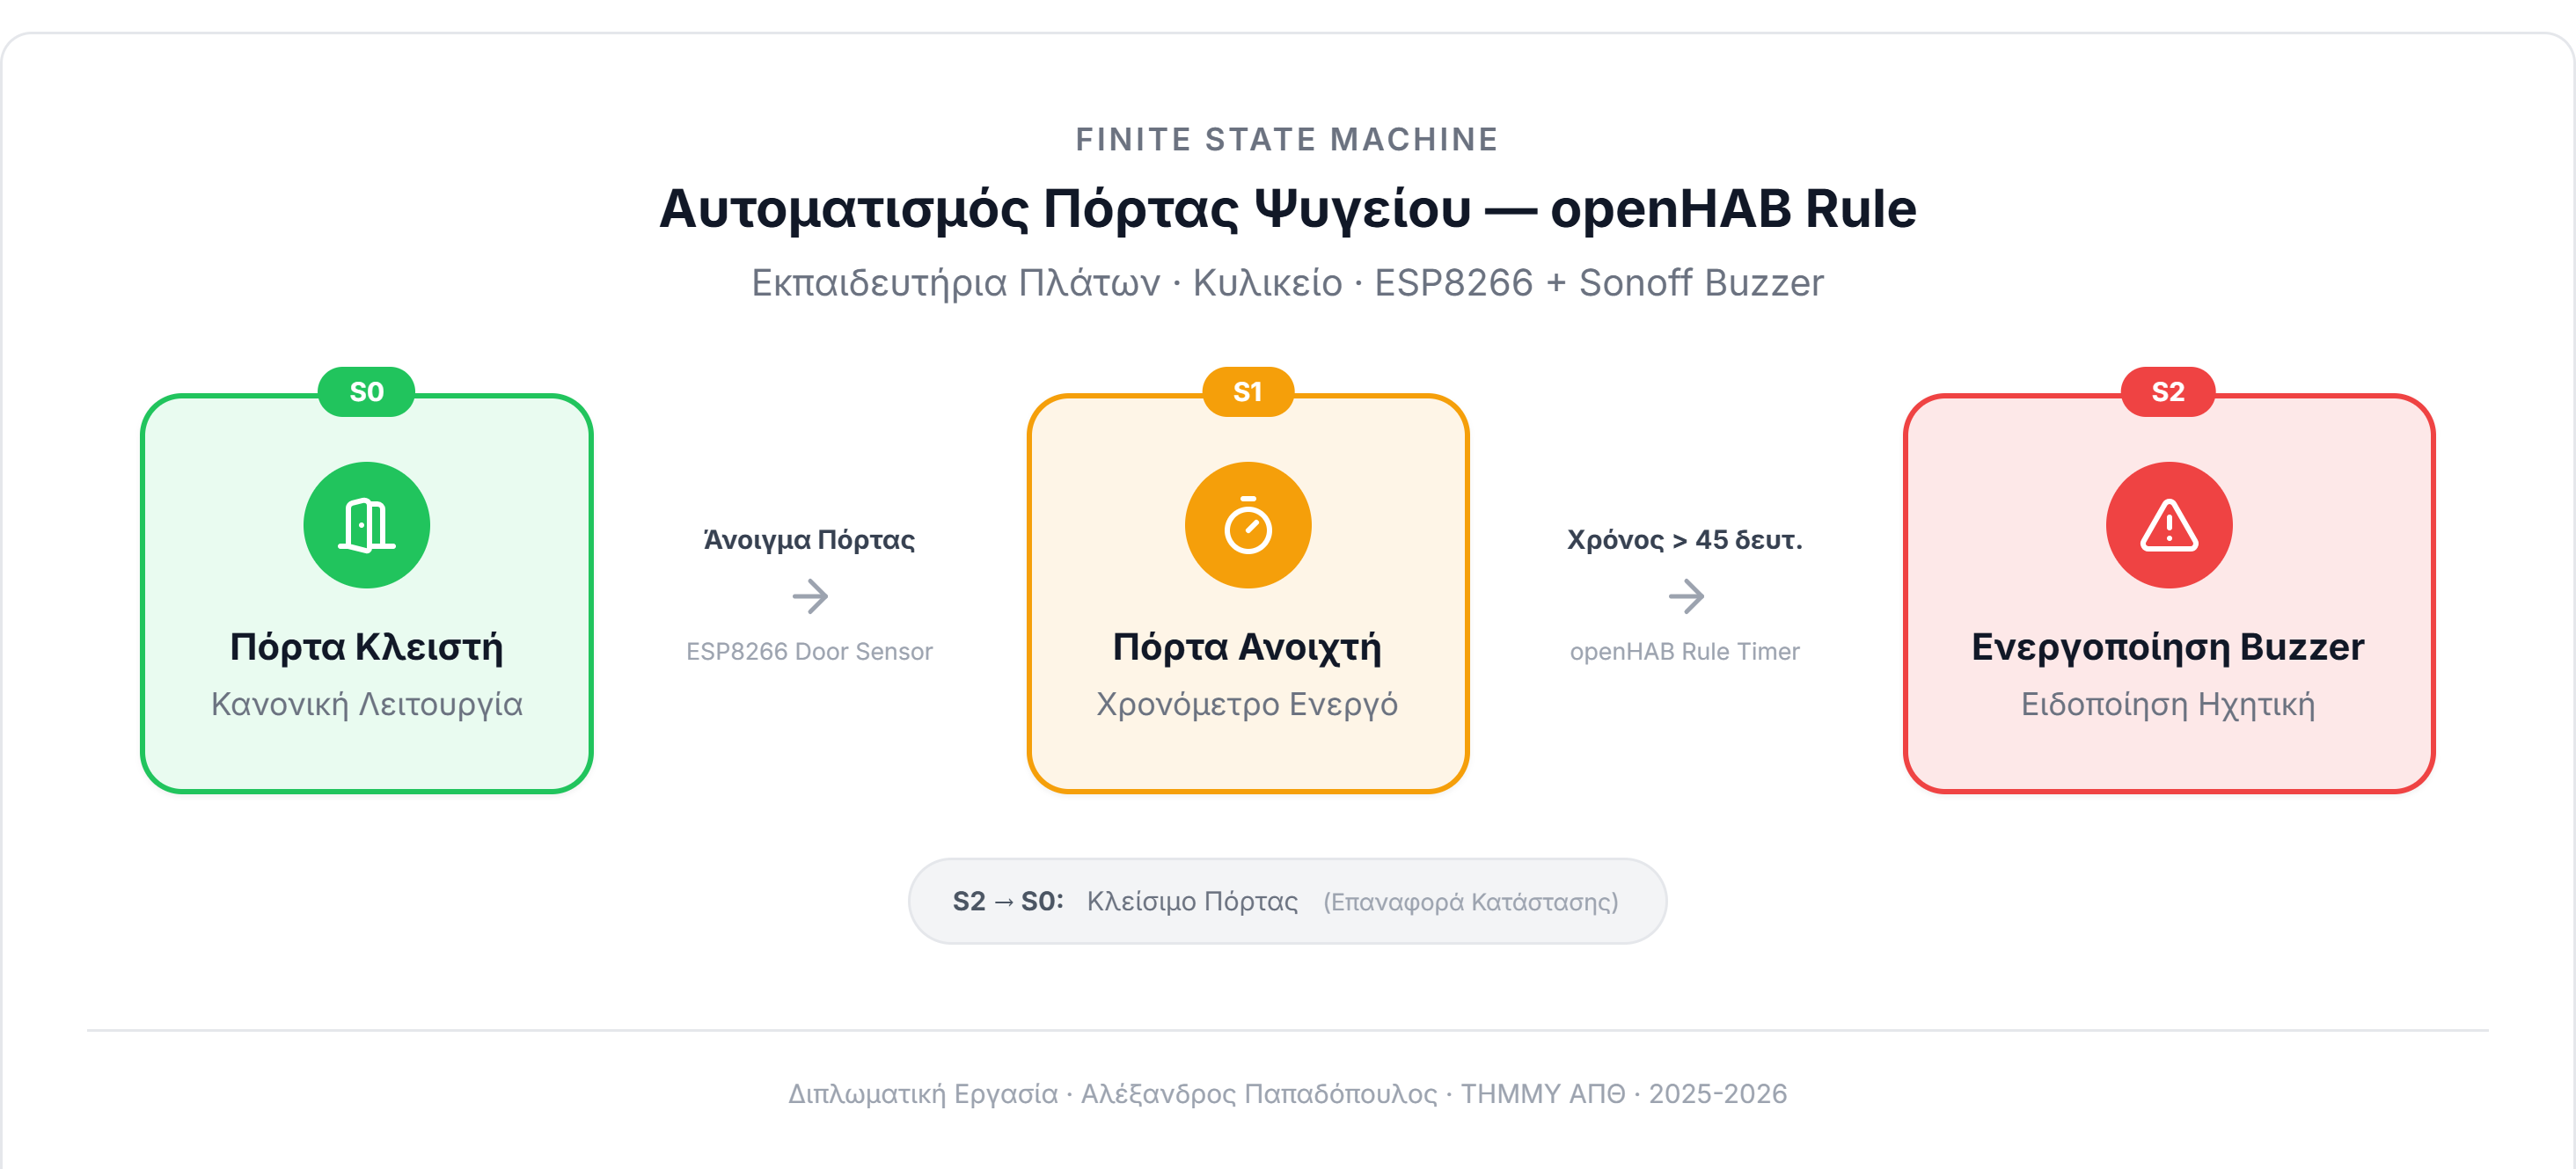
\includegraphics[width=\textwidth]{fig_4_1}
\caption{Απεικόνιση της λογικής κατάστασης του υποσυστήματος ελέγχου ψυγείου, όπως υλοποιήθηκε στο αρχικό \textlatin{proof-of-concept} επίπεδο.}
\label{fig:fridge_fsm}
\end{figure}

\begin{figure}[htbp]
\centering
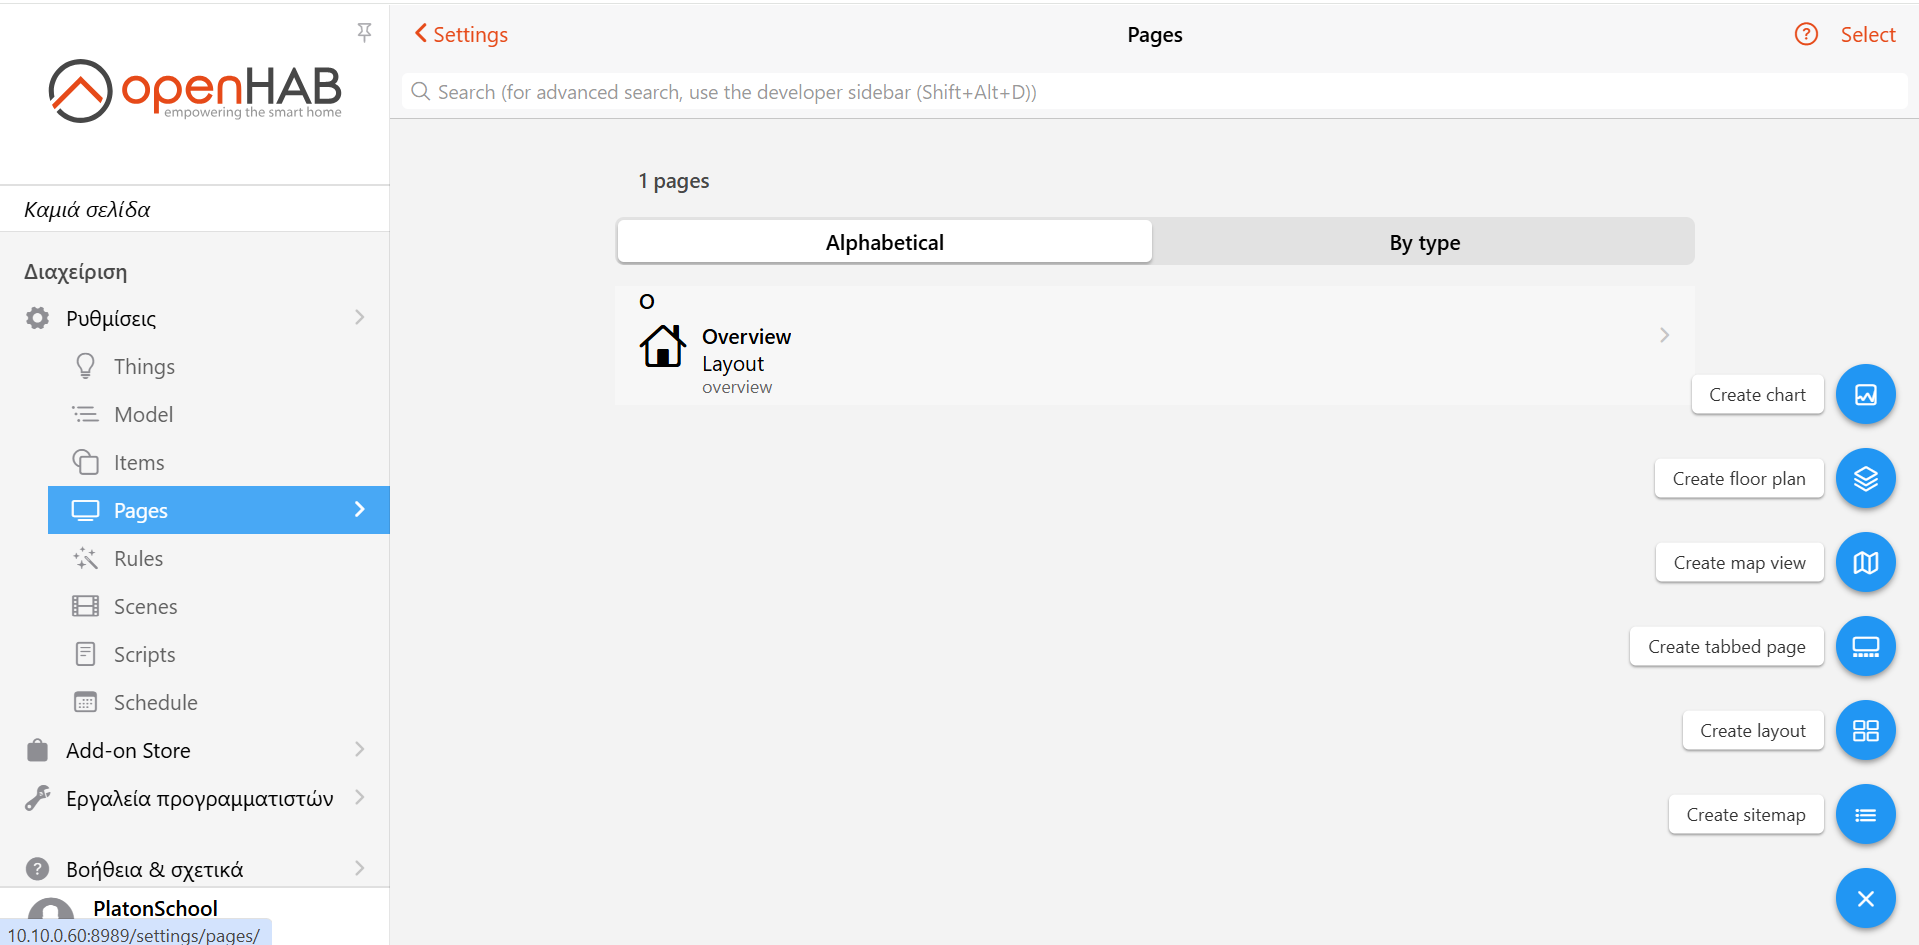
\includegraphics[width=\textwidth]{openhab_dashboard}
\caption{Ενδεικτική απεικόνιση του αρχικού \textlatin{engineering-oriented dashboard} του \textlatin{openHAB}, όπως χρησιμοποιήθηκε στο στάδιο του τοπικού πρωτοτύπου πριν από τη μετάβαση στη τελική \textlatin{cloud} διεπαφή.}
\label{fig:openhab_dashboard_legacy}
\end{figure}

\section{\texorpdfstring{Φάση 2: Ανάπτυξη \textlatin{Enterprise Cloud Platform (SaaS)}}{Φάση 2: Ανάπτυξη Enterprise Cloud Platform (SaaS)}}
Η δεύτερη φάση ανάπτυξης συνιστά τη μετάβαση από το τοπικό πρωτότυπο σε μια ώριμη \textlatin{cloud-based} πλατφόρμα, σχεδιασμένη να λειτουργεί ως ενιαίο περιβάλλον υπηρεσιών \textlatin{Smart Campus}. Σε αυτή τη φάση το βάρος μεταφέρθηκε από την τεχνική επαλήθευση του \textlatin{middleware} προς τη συνολική εμπειρία χρήστη, τη διαθεσιμότητα 24/7, τη δυνατότητα πρόσβασης από πολλαπλές συσκευές και την παροχή περισσότερο συγκεντρωτικών και επιχειρησιακά αξιοποιήσιμων προβολών.

Η νέα αρχιτεκτονική δεν ακυρώνει το τοπικό επίπεδο. Αντιθέτως, το διατηρεί ως αξιόπιστο μηχανισμό επικοινωνίας με το \textlatin{hardware}, ενώ μεταθέτει το επίπεδο παρουσίασης, υπηρεσιών και διαχείρισης σε \textlatin{cloud} περιβάλλον. Το \textlatin{openHAB} παραμένει συνεπώς κομβικό ως \textlatin{semantic middleware}, αλλά δεν αποτελεί πλέον το τελικό \textlatin{UI} της πλατφόρμας.

\subsection{\texorpdfstring{\textlatin{Frontend} με \textlatin{React 18, Vite} και \textlatin{Tailwind CSS}}{Frontend με React 18, Vite και Tailwind CSS}}
Το \textlatin{frontend} της νέας πλατφόρμας υλοποιήθηκε ως σύγχρονη \textlatin{Single-Page Application} βασισμένη σε \textlatin{React 18}, με εργαλείο δόμησης το \textlatin{Vite} και με χρήση \textlatin{Tailwind CSS} για τον οπτικό και \textlatin{responsive} σχεδιασμό της διεπαφής. Η επιλογή αυτής της στοίβας υπαγορεύθηκε από την ανάγκη για γρήγορη απόδοση στον \textlatin{browser}, αρθρωτή σύνθεση της διεπαφής και δυνατότητα ανάπτυξης εξειδικευμένων προβολών ανά ρόλο, υποσύστημα και σενάριο χρήσης.

Η νέα διεπαφή δεν αναπαράγει τη λογική ενός εργαλείου αυτοματισμού. Σχεδιάστηκε ώστε να υποστηρίζει λειτουργίες διοικητικής εποπτείας, παρακολούθησης κρίσιμων δεικτών, διαχείρισης συσκευών και πρόσβασης σε \textlatin{2D/3D} προβολές του σχολικού συγκροτήματος μέσα από ένα συνεκτικό περιβάλλον. Αυτή η μετατόπιση από \textlatin{system-centric} σε \textlatin{user-centric UX} αποτελεί έναν από τους βασικούς μετασχηματισμούς της πλατφόρμας.

\subsection{\texorpdfstring{\textlatin{Backend} με \textlatin{Supabase, PostgreSQL} και \textlatin{Edge Functions}}{Backend με Supabase, PostgreSQL και Edge Functions}}
Στο \textlatin{backend} επίπεδο η πλατφόρμα μεταφέρθηκε σε υποδομή νέφους με \textlatin{Supabase} και \textlatin{PostgreSQL}. Η επιλογή αυτή επέτρεψε την ενοποιημένη αποθήκευση επιχειρησιακών δεδομένων, τη διαχείριση χρηστών και ρόλων, καθώς και τη δημιουργία προσαρμοσμένων \textlatin{cloud services} που συνδέουν το \textlatin{semantic middleware} επίπεδο με το τελικό περιβάλλον χρήσης. Σημαντικό μέρος αυτής της φάσης αποτελεί η χρήση \textlatin{Edge Functions}, όπως η \textlatin{\texttt{openhab-sync}}, για τη συγχρονισμένη μεταφορά και ανανέωση δεδομένων από το \textlatin{openHAB} προς το \textlatin{cloud} επίπεδο υπηρεσιών.

Η επιλογή του οικοσυστήματος \textlatin{PostgreSQL} σηματοδοτεί επίσης μια ουσιαστική μετατόπιση από την αποκλειστική λογική \textlatin{time-series persistence} προς ένα πλουσιότερο \textlatin{cloud data model}, στο οποίο τα δεδομένα του \textlatin{Digital Twin} μπορούν να συνδυάζονται με \textlatin{metadata}, ρόλους, χώρους, συσκευές και ιστορικά γεγονότα μέσα σε ένα περισσότερο \textlatin{enterprise-ready} μοντέλο.

Η πλήρης δομή της βάσης δεδομένων αποτυπώνεται στο Διάγραμμα Οντοτήτων-Σχέσεων (\textlatin{Entity-Relationship Diagram}) του Σχήματος~4.8, το οποίο περιλαμβάνει τους βασικούς πίνακες: \textlatin{organizations, organization\_members, digital\_twins, sensors, sensor\_readings, assets, events, rules, και openhab\_config}. Κάθε πίνακας φέρει \textlatin{org\_id} ως \textlatin{foreign key} για την εφαρμογή πολιτικών \textlatin{RLS}.

\subsection{\textlatin{Multi-tenancy, RBAC} και έλεγχος πρόσβασης}
Στο \textlatin{cloud} επίπεδο ενσωματώθηκε αυστηρότερη λογική ελέγχου πρόσβασης με \textlatin{Role-Based Access Control} και \textlatin{Row-Level Security}, ώστε η πλατφόρμα να υποστηρίζει απομονωμένη πρόσβαση ανά χρήστη, χώρο και οργανωτική μονάδα. Η λογική αυτή δεν σχεδιάστηκε μόνο για το παρόν \textlatin{case study}, αλλά και ως αρχιτεκτονική πρόβλεψη για πιθανή επέκταση σε περισσότερα από ένα σχολικά συγκροτήματα ή σε μελλοντικό περιβάλλον \textlatin{multi-tenant}.

Το αποτέλεσμα είναι ότι οι τεχνικές λειτουργίες διαχείρισης, οι καθημερινές προβολές διοίκησης και τα εξειδικευμένα \textlatin{panels} μπορούν να διατίθενται επιλεκτικά, με σαφή διαχωρισμό μεταξύ \textlatin{administrators}, \textlatin{operation users} και απλών χρηστών παρακολούθησης. Με αυτόν τον τρόπο, η πλατφόρμα αποκτά χαρακτήρα πραγματικής υπηρεσίας \textlatin{SaaS} και όχι απλώς απομακρυσμένου \textlatin{engineering dashboard}. Μια κεντρική επισκόπηση αυτής της νέας διεπαφής παρουσιάζεται στο Σχήμα~\ref{fig:smart_campus_dashboard}. Το Σχήμα 4.3 παρουσιάζει την κεντρική επισκόπηση (\textlatin{Overview}) της πλατφόρμας. Τέσσερα στοιχεία αξίζουν ιδιαίτερης προσοχής: πρώτον, η κάρτα κατάστασης σχολείου (Ανοιχτό/Κλειστό) που αποδεικνύει ότι το σύστημα είναι \textlatin{context-aware} και προσαρμόζεται αυτόματα στο σχολικό ωράριο· δεύτερον, ο αριθμός των \textlatin{online} αισθητήρων με \textlatin{Live} badge που επιβεβαιώνει ότι υπάρχει πραγματική \textlatin{IoT} υποδομή· τρίτον, η μηνιαία κατανάλωση ενέργειας (\textlatin{kWh}) ως κεντρικό \textlatin{KPI} που συνδέεται άμεσα με τη μείωση 19,7\% που πέτυχε το σύστημα· και τέταρτον, η χαρτογράφηση του \textlatin{campus} με \textlatin{zones} που αποδεικνύει τη χωρική επίγνωση (\textlatin{spatial awareness}) του Ψηφιακού Διδύμου.

\begin{figure}[htbp]
\centering
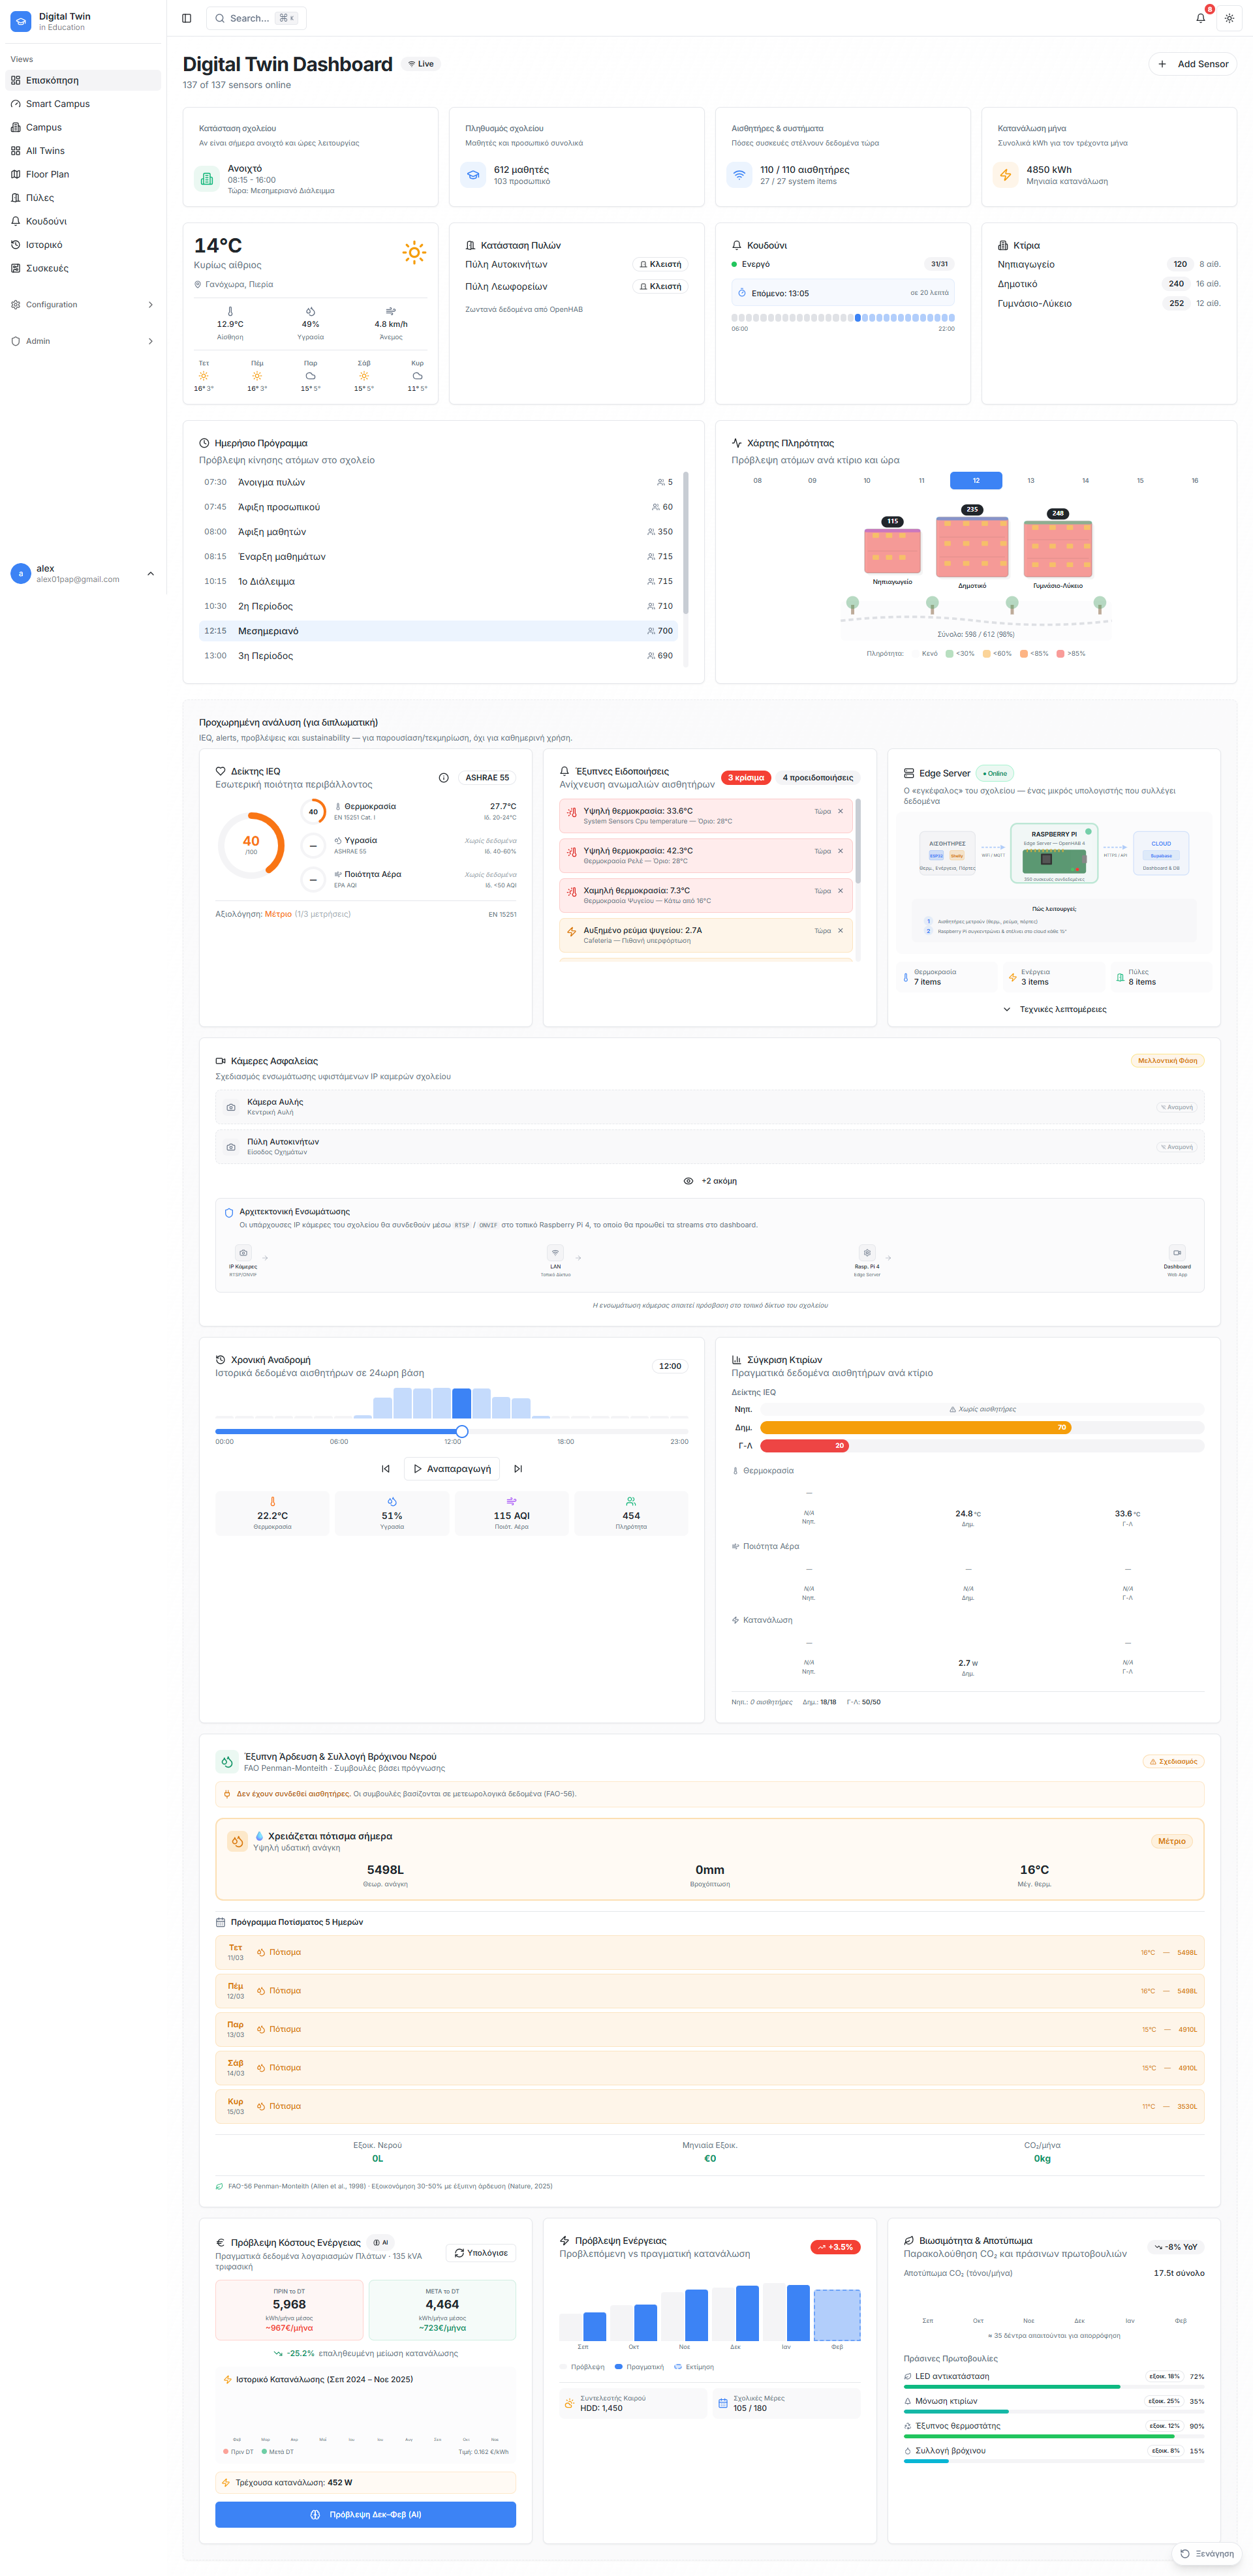
\includegraphics[width=\textwidth]{fig_4_2}
\caption{Κεντρική επισκόπηση της \textlatin{cloud-based} πλατφόρμας \textlatin{Smart Campus} με συγκεντρωτικούς δείκτες, ειδοποιήσεις και λειτουργικές προβολές.}
\label{fig:smart_campus_dashboard}
\end{figure}

\section{\texorpdfstring{Οπτικοποίηση και \textlatin{3D} Ψηφιακό Δίδυμο}{Οπτικοποίηση και 3D Ψηφιακό Δίδυμο}}
Η τελική μορφή της πλατφόρμας αποδίδει ιδιαίτερη σημασία στο επίπεδο οπτικοποίησης, καθώς αυτό είναι το σημείο στο οποίο το τεχνικό υπόβαθρο του \textlatin{Digital Twin} μετασχηματίζεται σε εργαλείο καθημερινής επιχειρησιακής χρήσης. Για τον λόγο αυτό, το \textlatin{visual layer} υλοποιήθηκε όχι ως παθητική συλλογή γραφημάτων, αλλά ως συνδυασμός \textlatin{2D} και \textlatin{3D} προβολών που αποτυπώνουν τον χώρο, τις συσκευές και τη ζωντανή κατάσταση της εγκατάστασης.

\subsection{\texorpdfstring{\textlatin{React Three Fiber} και \textlatin{Isometric Campus View}}{React Three Fiber και Isometric Campus View}}
Για την τρισδιάστατη απεικόνιση χρησιμοποιήθηκε το \textlatin{React Three Fiber (R3F)}, το οποίο επιτρέπει τη γεφύρωση της λογικής \textlatin{component-based} ανάπτυξης του \textlatin{React} με τη μηχανή γραφικών \textlatin{Three.js} \cite{PMNDRS2024}. Η επιλογή αυτή δικαιολογείται από τη δυνατότητα ανάπτυξης παραμετρικών τρισδιάστατων σκηνών, όπου τα κτίρια, οι χώροι και οι συσκευές δεν αποτυπώνονται απλώς ως στατικά μοντέλα, αλλά ως διαδραστικά στοιχεία που ενημερώνονται σε πραγματικό χρόνο.

Στο επίπεδο αυτό αναπτύχθηκε \textlatin{isometric campus view}, μέσω της οποίας ο χρήστης μπορεί να αποκτήσει συνολική αντίληψη της εγκατάστασης, να εντοπίσει κρίσιμα συμβάντα και να πλοηγηθεί λειτουργικά από το επίπεδο του \textlatin{campus} σε επιμέρους κτίρια και δωμάτια. Η \textlatin{3D} απεικόνιση υπηρετεί έτσι όχι μόνο αισθητικούς στόχους, αλλά κυρίως στόχους χωρικής επίγνωσης και επιχειρησιακής απόκρισης.

\subsection{\texorpdfstring{\textlatin{2D Interactive Floorplans}}{2D Interactive Floorplans}}
Παράλληλα με την τρισδιάστατη προβολή, υλοποιήθηκαν διαδραστικά \textlatin{2D floorplans} που λειτουργούν ως άμεσος μηχανισμός πλοήγησης για καθημερινά σενάρια διαχείρισης. Το \textlatin{floor plan} του σχολικού συγκροτήματος εμφανίζει τη συνολική διάταξη των χώρων και την κατάσταση κάθε αίθουσας, δηλαδή αν λειτουργεί ως ενεργό \textlatin{Digital Twin} ή όχι. Ο χρήστης μπορεί να επιλέξει οποιαδήποτε αίθουσα για να μεταβεί στην αναλυτική προβολή του αντίστοιχου υποσυστήματος.

Η συνύπαρξη \textlatin{3D} και \textlatin{2D} προβολών εξυπηρετεί διαφορετικά επίπεδα χωρικής πλοήγησης. Το Σχήμα 4.4 αποδίδει την τρισδιάστατη προβολή του \textlatin{campus}, ενώ το Σχήμα 4.5 παρουσιάζει το \textlatin{floor plan} με την κατάσταση κάθε αίθουσας --- οι χώροι που λειτουργούν ως ενεργά \textlatin{Digital Twins} επισημαίνονται διακριτά, επιτρέποντας στον χρήστη να εισέλθει σε κάθε έναν για αναλυτική παρακολούθηση.

\begin{figure}[htbp]
\centering
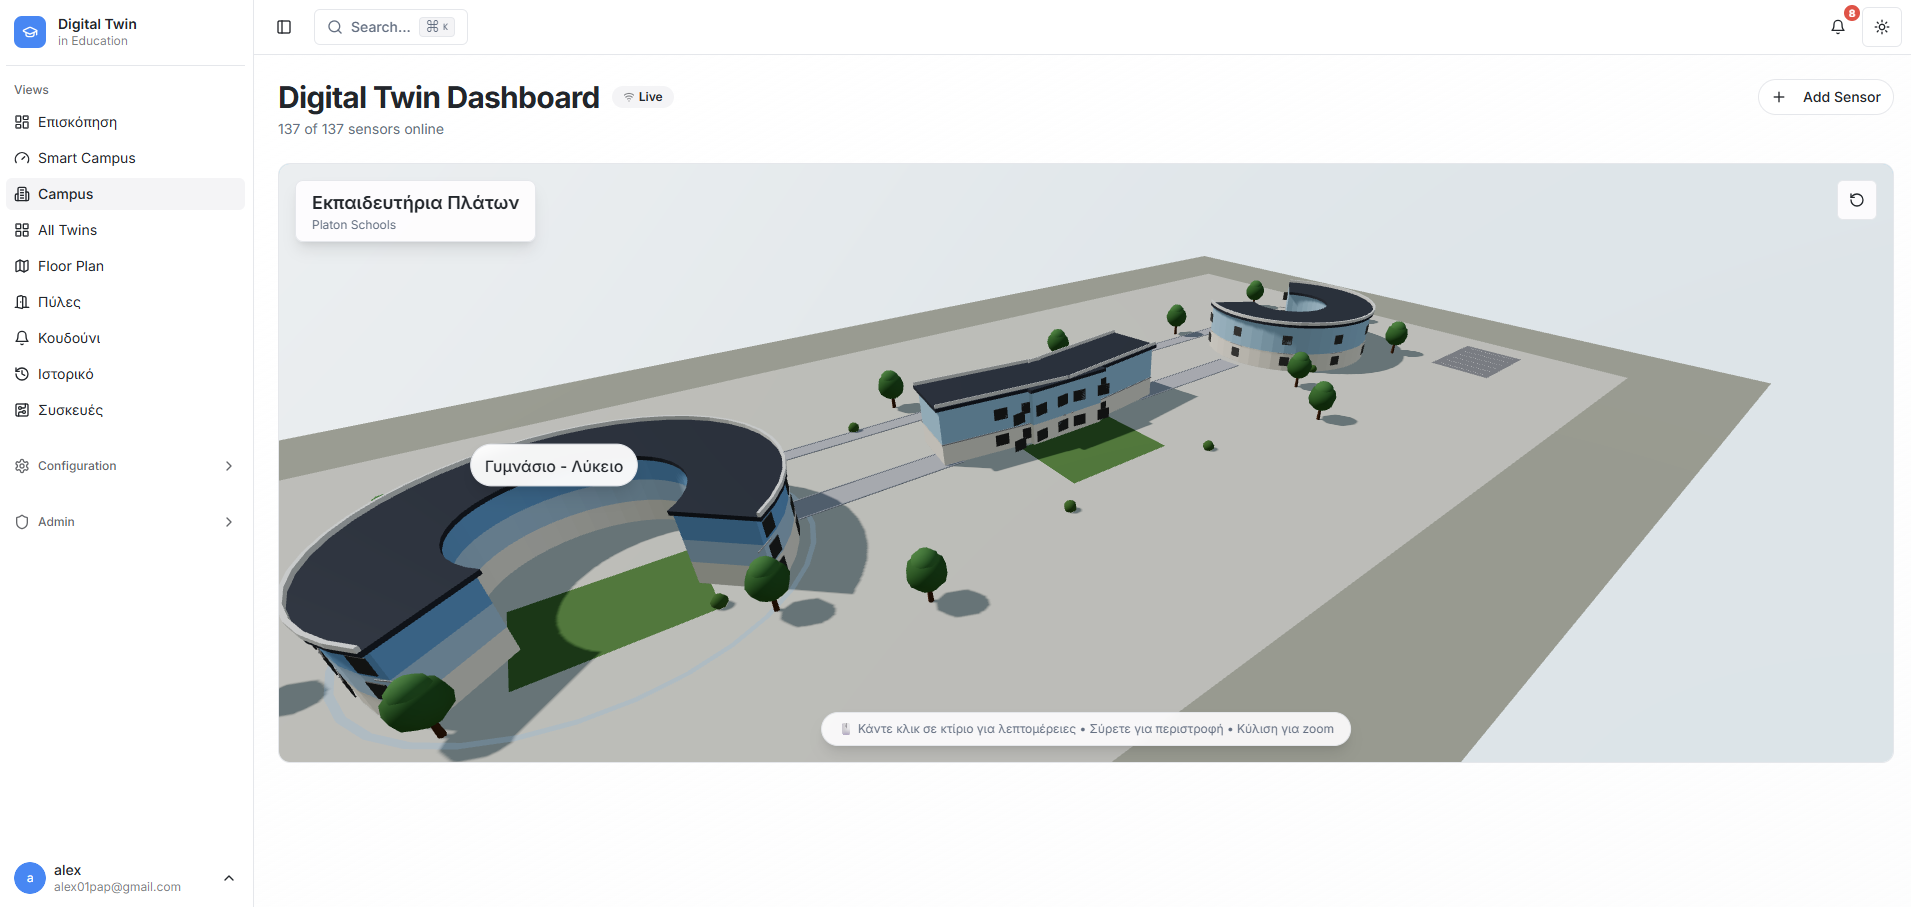
\includegraphics[width=\textwidth]{fig_1_1}
\caption{Τρισδιάστατη απεικόνιση του \textlatin{campus} των Εκπαιδευτηρίων Πλάτων --- ο χρήστης μπορεί να πλοηγηθεί στο μοντέλο και να επιλέξει κτίριο για αναλυτική προβολή.}
\label{fig:campus_view_3d}
\end{figure}

\begin{figure}[htbp]
\centering
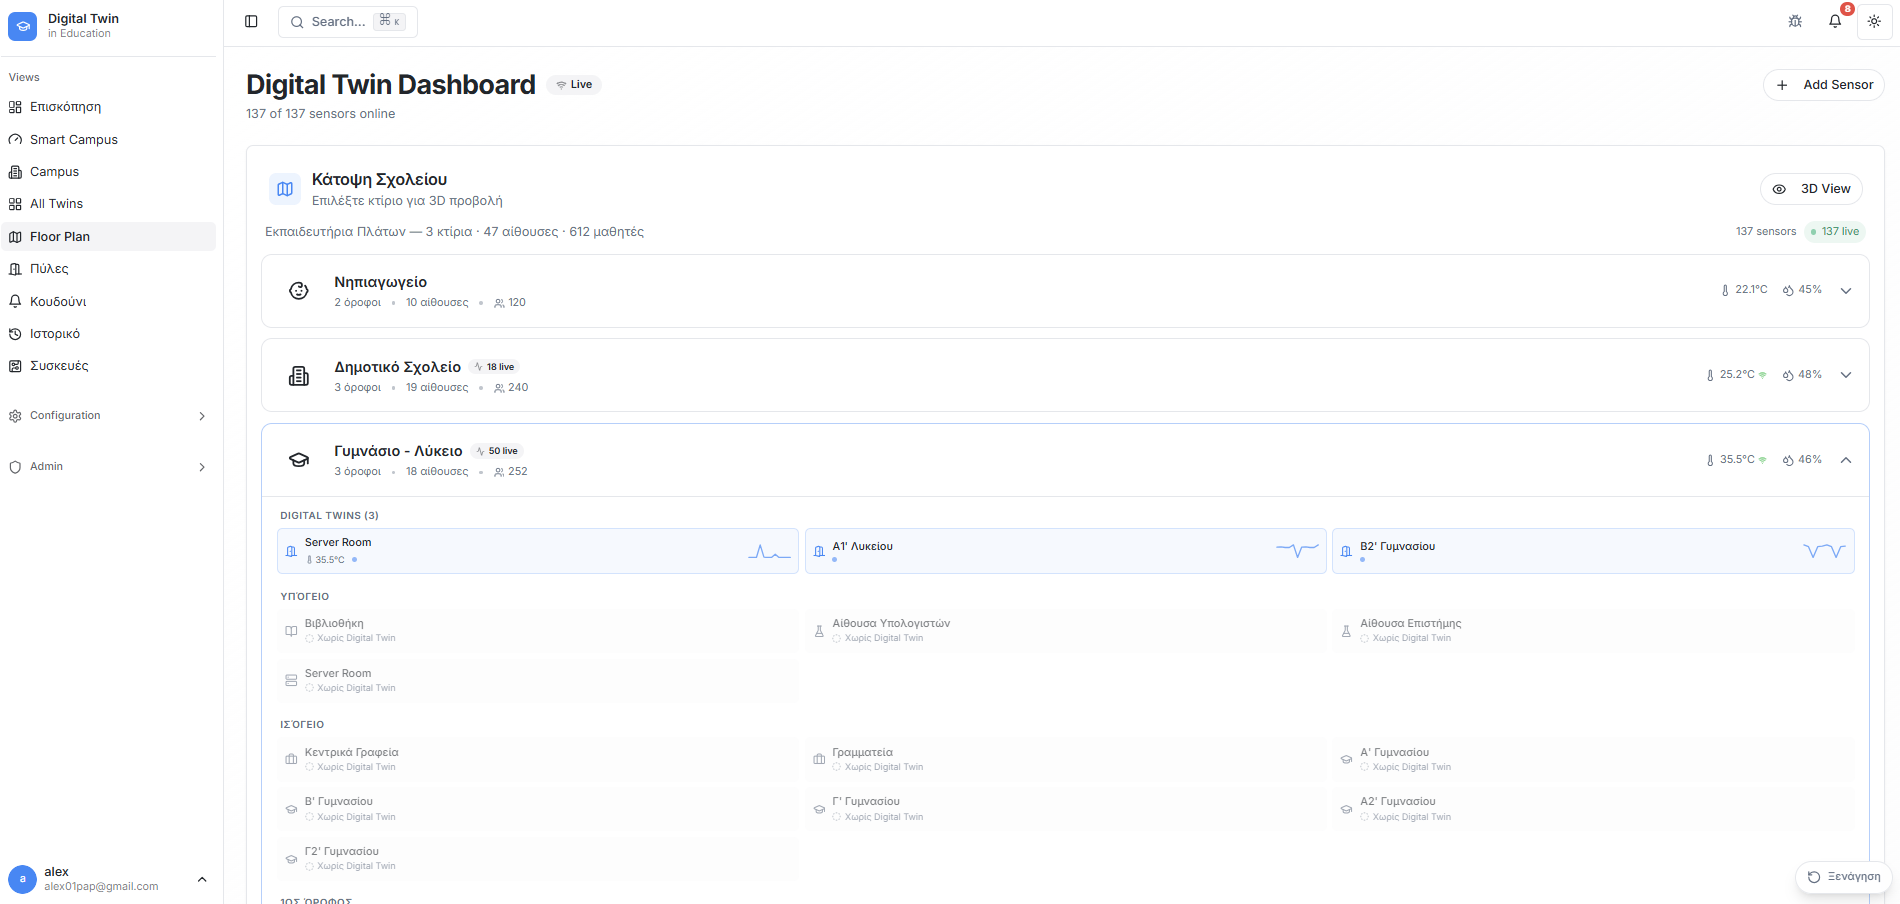
\includegraphics[width=\textwidth]{Screenshot_1}
\caption{\textlatin{Floor plan} του σχολικού συγκροτήματος --- κάθε αίθουσα εμφανίζεται με την κατάστασή της (\textlatin{live Digital Twin} ή όχι) και επιτρέπει την πλοήγηση στο αντίστοιχο υποσύστημα.}
\label{fig:campus_floorplan_2d}
\end{figure}

\section{\texorpdfstring{Διαλειτουργικότητα, \textlatin{AI} και Εμπειρία Χρήστη}{Διαλειτουργικότητα, AI και Εμπειρία Χρήστη}}
Η τελική μορφή της πλατφόρμας διαφοροποιείται ουσιαστικά από ένα συμβατικό σύστημα εποπτείας, επειδή ενσωματώνει ετερογενή υποσυστήματα, επεκτείνεται με αλγοριθμικά εργαλεία και προσφέρει συνεκτική εμπειρία χρήσης σε πολλαπλές κατηγορίες χρηστών. Η ενότητα αυτή παρουσιάζει τρία από τα βασικότερα ώριμα χαρακτηριστικά της: τη διαλειτουργικότητα με \textlatin{legacy} υποδομές, την εισαγωγή λειτουργιών \textlatin{AI} και τη \textlatin{responsive} φύση της διεπαφής.

\subsection{\texorpdfstring{\textlatin{Brownfield Integration} και ενοποίηση υφιστάμενων συστημάτων}{Brownfield Integration και ενοποίηση υφιστάμενων συστημάτων}}
Η αναπτυχθείσα πλατφόρμα δεν σχεδιάστηκε με λογική αντικατάστασης όλων των προϋπαρχόντων συστημάτων. Αντίθετα, υιοθετήθηκε αρχιτεκτονική \textlatin{Brownfield Integration}, σύμφωνα με την οποία υφιστάμενες υποδομές, όπως οι αυτόματες πύλες του σχολείου, μπορούν να ενταχθούν στο ενιαίο οικοσύστημα ελέγχου καθαρά μέσω λογισμικού και διασύνδεσης. Η προσέγγιση αυτή μειώνει το κόστος μετάβασης, ενισχύει τη διαλειτουργικότητα και επιτρέπει στην πλατφόρμα να λειτουργεί ως κοινός \textlatin{operational} χώρος για πολλαπλά υποσυστήματα.

Στην ίδια λογική εντάσσεται και η δυνατότητα επέκτασης προς κάμερες, \textlatin{irrigation logic} και άλλες λειτουργίες \textlatin{campus management}. Το κεντρικό μήνυμα είναι ότι το ψηφιακό δίδυμο δεν περιορίζεται στη συλλογή αισθητηριακών δεδομένων, αλλά τείνει να εξελιχθεί σε λογισμικό ενοποίησης διαφορετικών τεχνολογικών νησίδων.

\subsection{\texorpdfstring{\textlatin{Device Management} και λειτουργικές καρτέλες ελέγχου}{Device Management και λειτουργικές καρτέλες ελέγχου}}
Η καρτέλα Συσκευών (\textlatin{Devices}) λειτουργεί ως \textlatin{hardware inventory} και \textlatin{health monitor} της \textlatin{IoT} υποδομής. Παρέχει πλήρη ορατότητα σε όλο το φυσικό \textlatin{hardware} που τροφοδοτεί το Ψηφιακό Δίδυμο, από τον \textlatin{edge server} έως τους τερματικούς αισθητήρες και τα ρελέ.

Συγκεκριμένα, η καρτέλα περιλαμβάνει: (α) κατάλογο συσκευών με κάρτα για κάθε \textlatin{device} (\textlatin{Raspberry Pi 4}, \textlatin{ESP32}, \textlatin{Shelly 1PM}, μαγνητικές επαφές, \textlatin{DFPlayer}) που εμφανίζει \textlatin{specs}, πρωτόκολλο επικοινωνίας και τοποθεσία εγκατάστασης, (β) \textlatin{live telemetry} από το \textlatin{openHAB} με πραγματικές τιμές κατάστασης (\textlatin{online/offline}) και τελευταίες μετρήσεις ανά συσκευή, (γ) 24ωρο \textlatin{uptime timeline} που αποτυπώνει οπτικά την ιστορία διαθεσιμότητας κάθε κόμβου, (δ) διάγραμμα τοπολογίας δικτύου που δείχνει τη ροή δεδομένων από τους αισθητήρες προς τον \textlatin{edge server} και το \textlatin{cloud}, και (ε) τρισδιάστατη προβολή των \textlatin{hardware components} για άμεση οπτική αναγνώριση του εξοπλισμού.

Η καρτέλα αυτή τεκμηριώνει ότι το Ψηφιακό Δίδυμο στηρίζεται σε πραγματική, επαληθεύσιμη \textlatin{IoT} υποδομή. Ο αναγνώστης μπορεί να επιβεβαιώσει ακριβώς ποιο \textlatin{hardware} χρησιμοποιήθηκε, πού τοποθετήθηκε και αν λειτουργεί σωστά σε πραγματικό χρόνο.

\begin{figure}[htbp]
\centering
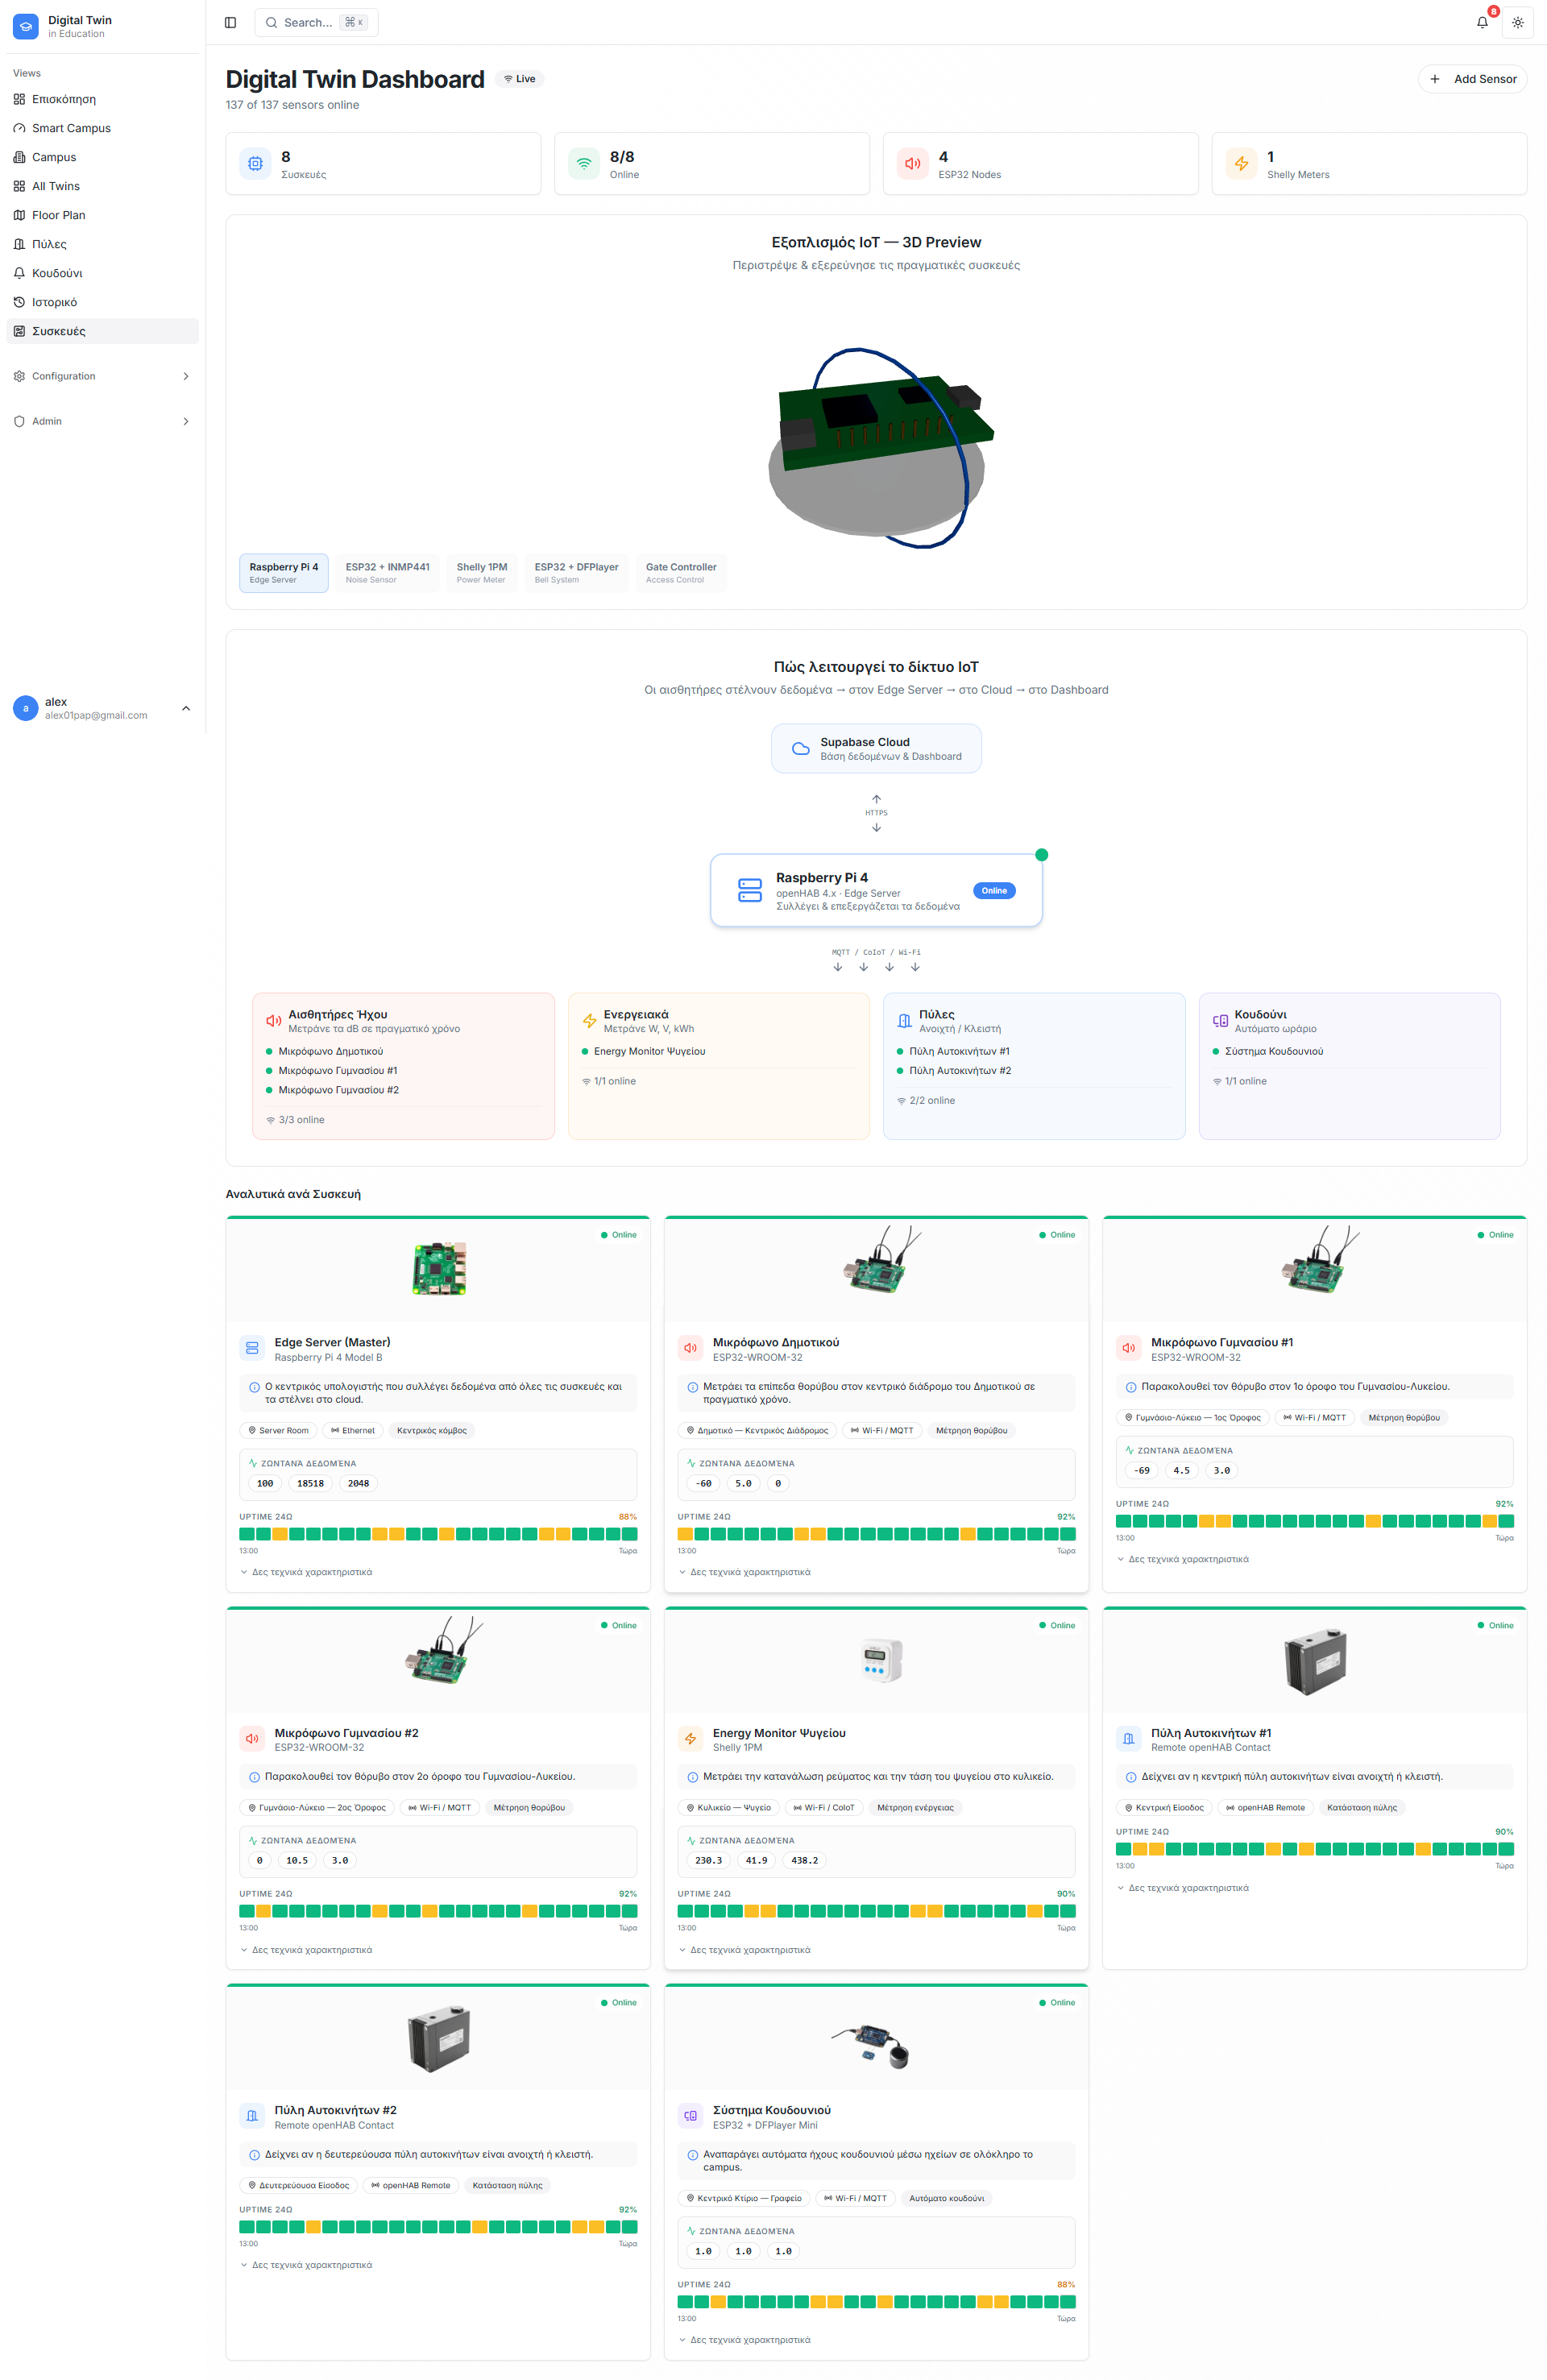
\includegraphics[width=0.76\textwidth]{fig_4_5}

\vspace{0.5em}

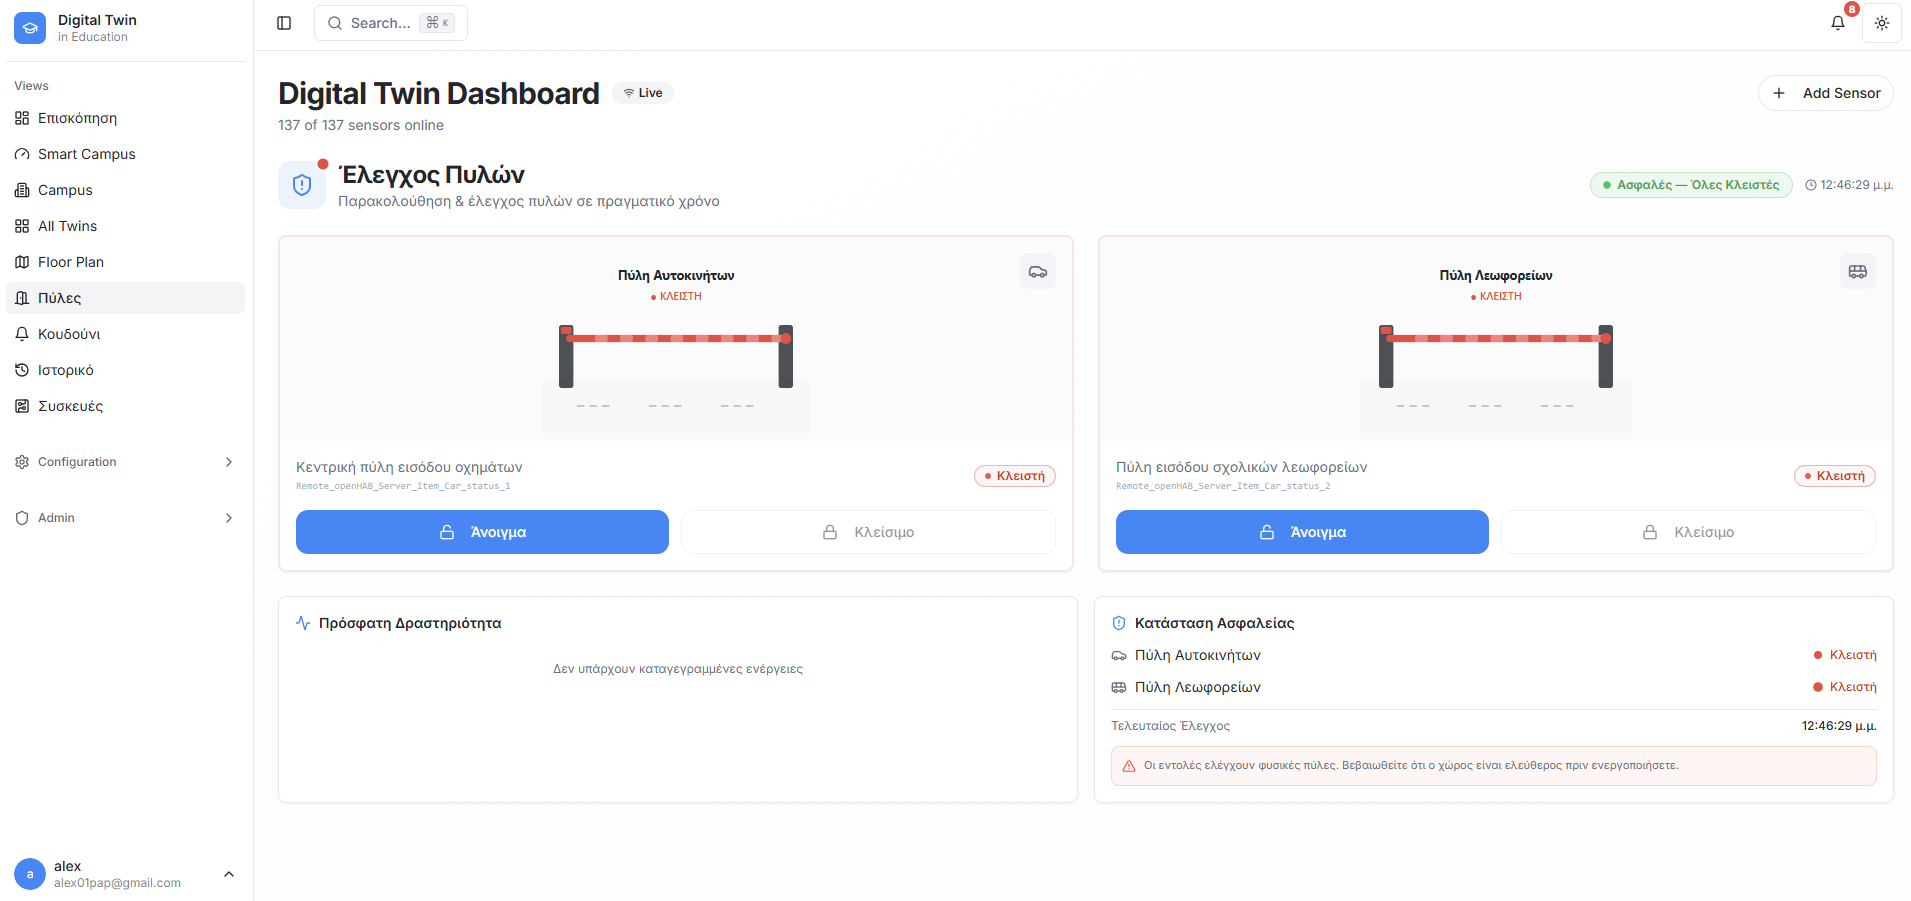
\includegraphics[width=0.76\textwidth]{fig_4_51}
\caption{Ενδεικτική παρουσίαση των καρτελών διαχείρισης συσκευών και της διεπαφής ελέγχου πυλών στο cloud περιβάλλον της πλατφόρμας.}
\label{fig:device_management}
\end{figure}

\subsection{\texorpdfstring{Widgets ενεργειακής πρόβλεψης και \textlatin{LLM-based forecasting}}{Widgets ενεργειακής πρόβλεψης και LLM-based forecasting}}
Το σύστημα διαθέτει δύο widgets ενεργειακής πρόβλεψης. Το πρώτο (\textlatin{PredictiveEnergy}) παρέχει οπτική σύγκριση προβλεπόμενης έναντι πραγματικής κατανάλωσης βάσει ιστορικών δεδομένων με \textlatin{animated bar chart}. Το δεύτερο (\textlatin{EnergyCostPrediction}) αξιοποιεί \textlatin{LLM-based forecasting} μέσω του \textlatin{Gemini API}, το οποίο λαμβάνει τα πραγματικά \textlatin{billing data} της εγκατάστασης και παράγει δομημένες προβλέψεις (\textlatin{JSON}) για ορίζοντα 3 μηνών, λαμβάνοντας υπόψη το ελληνικό τιμολόγιο ενέργειας (0,162 €/\textlatin{kWh}), το σχολικό ημερολόγιο, την εποχικότητα και τον επαληθευμένο συντελεστή μείωσης 19,7\%.

Η προσέγγιση αυτή αποτελεί \textlatin{LLM-as-a-forecaster} με \textlatin{domain knowledge}, όχι κλασικό στατιστικό μοντέλο τύπου \textlatin{ARIMA} ή \textlatin{LSTM}. Η λειτουργία αυτή οπτικοποιείται στο Σχήμα~\ref{fig:ai_energy_forecasting}.

\begin{figure}[htbp]
\centering
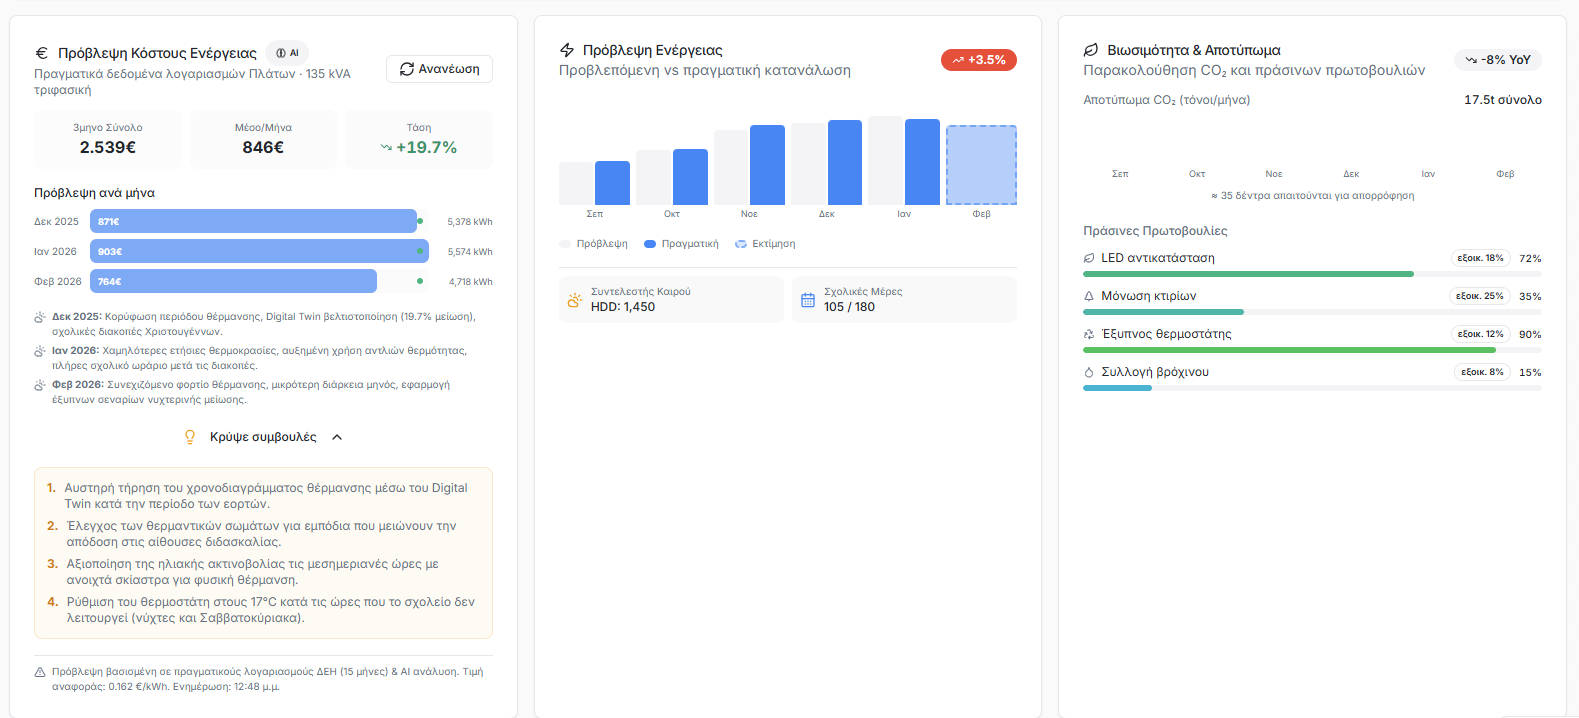
\includegraphics[width=0.78\textwidth]{fig_4_6}

\vspace{0.5em}

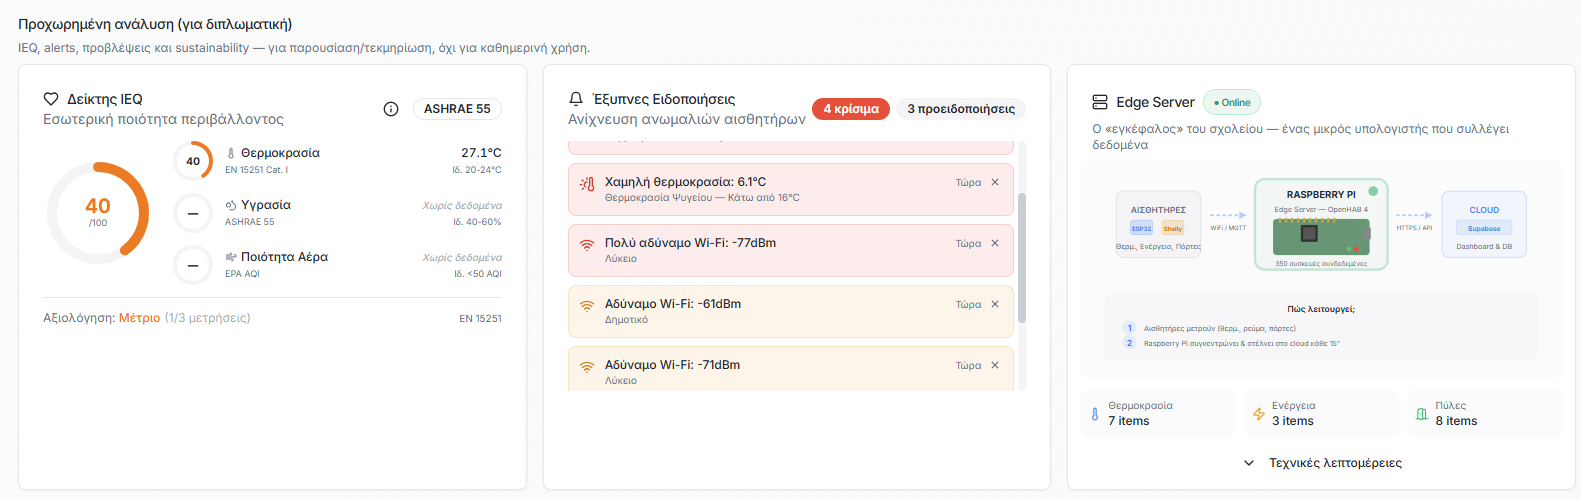
\includegraphics[width=0.78\textwidth]{fig_4_61}
\caption{Ενδεικτική απεικόνιση των δύο widgets ενεργειακής πρόβλεψης της πλατφόρμας: \textlatin{PredictiveEnergy} και \textlatin{EnergyCostPrediction}.}
\label{fig:ai_energy_forecasting}
\end{figure}

\subsection{\texorpdfstring{\textlatin{Responsive} πρόσβαση και χρήση από μη τεχνικούς ρόλους}{Responsive πρόσβαση και χρήση από μη τεχνικούς ρόλους}}
Σε αντίθεση με την πρώτη φάση, κατά την οποία η απομακρυσμένη τεχνική πρόσβαση στο τοπικό πρωτότυπο απαιτούσε περισσότερο εξειδικευμένη δικτυακή διαχείριση, η τελική \textlatin{cloud} πλατφόρμα σχεδιάστηκε ώστε να είναι άμεσα προσβάσιμη μέσω \textlatin{browser}, χωρίς να απαιτείται \textlatin{VPN} για τον τελικό χρήστη. Η \textlatin{responsive} φύση της εφαρμογής επιτρέπει χρήση από κινητά τηλέφωνα, \textlatin{tablets} και σταθμούς εργασίας, διασφαλίζοντας ότι η πλατφόρμα μπορεί να χρησιμοποιηθεί καθημερινά από διευθυντές και προσωπικό λειτουργίας, όχι μόνο από μηχανικούς ή τεχνικούς.

Αυτό το χαρακτηριστικό δεν αποτελεί απλή βελτίωση εργονομίας. Αντιπροσωπεύει μία ουσιώδη αλλαγή στο ίδιο το \textlatin{operational} μοντέλο της πλατφόρμας. Η πληροφορία και ο έλεγχος γίνονται πλέον διαθέσιμα στο σημείο λήψης αποφάσεων, γεγονός που αυξάνει τη χρηστικότητα, επιταχύνει την απόκριση σε συμβάντα και διευρύνει σημαντικά το πεδίο πρακτικής υιοθέτησης της πλατφόρμας. Η \textlatin{responsive} συμπεριφορά της πλατφόρμας απεικονίζεται στο Σχήμα~\ref{fig:responsive_views}.

\begin{figure}[htbp]
\centering
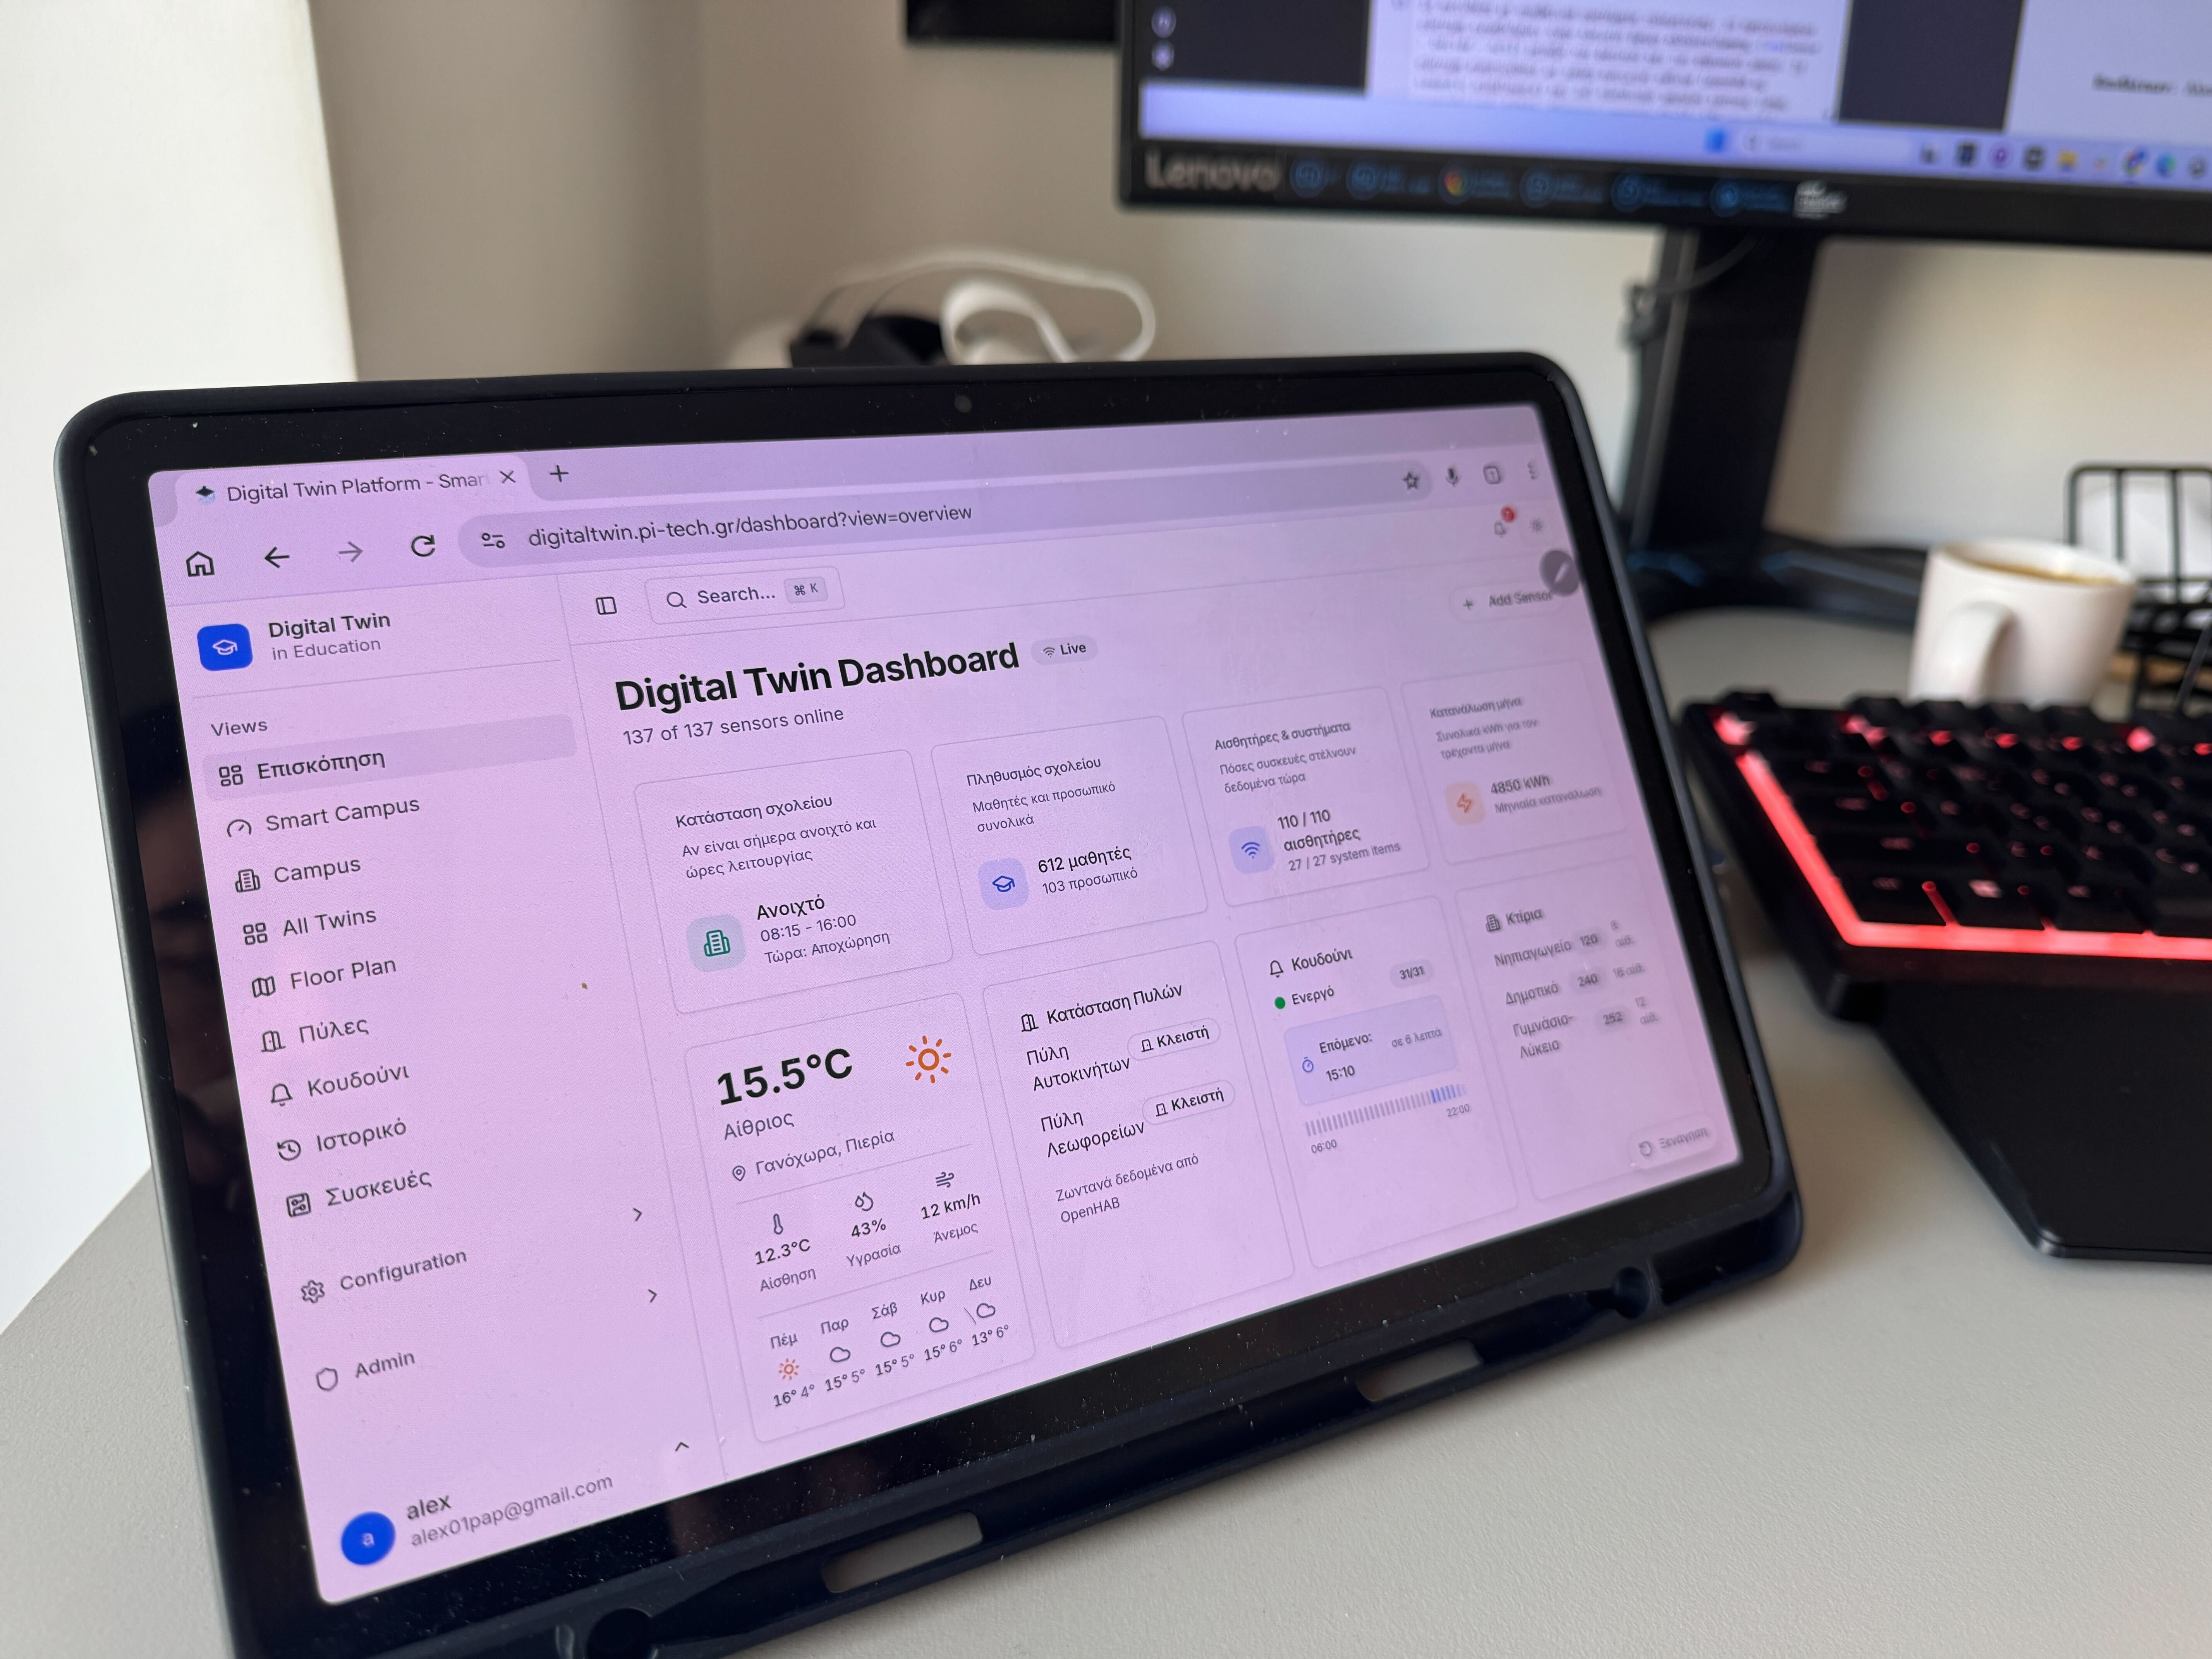
\includegraphics[width=0.31\textwidth]{fig_4_4}\hfill
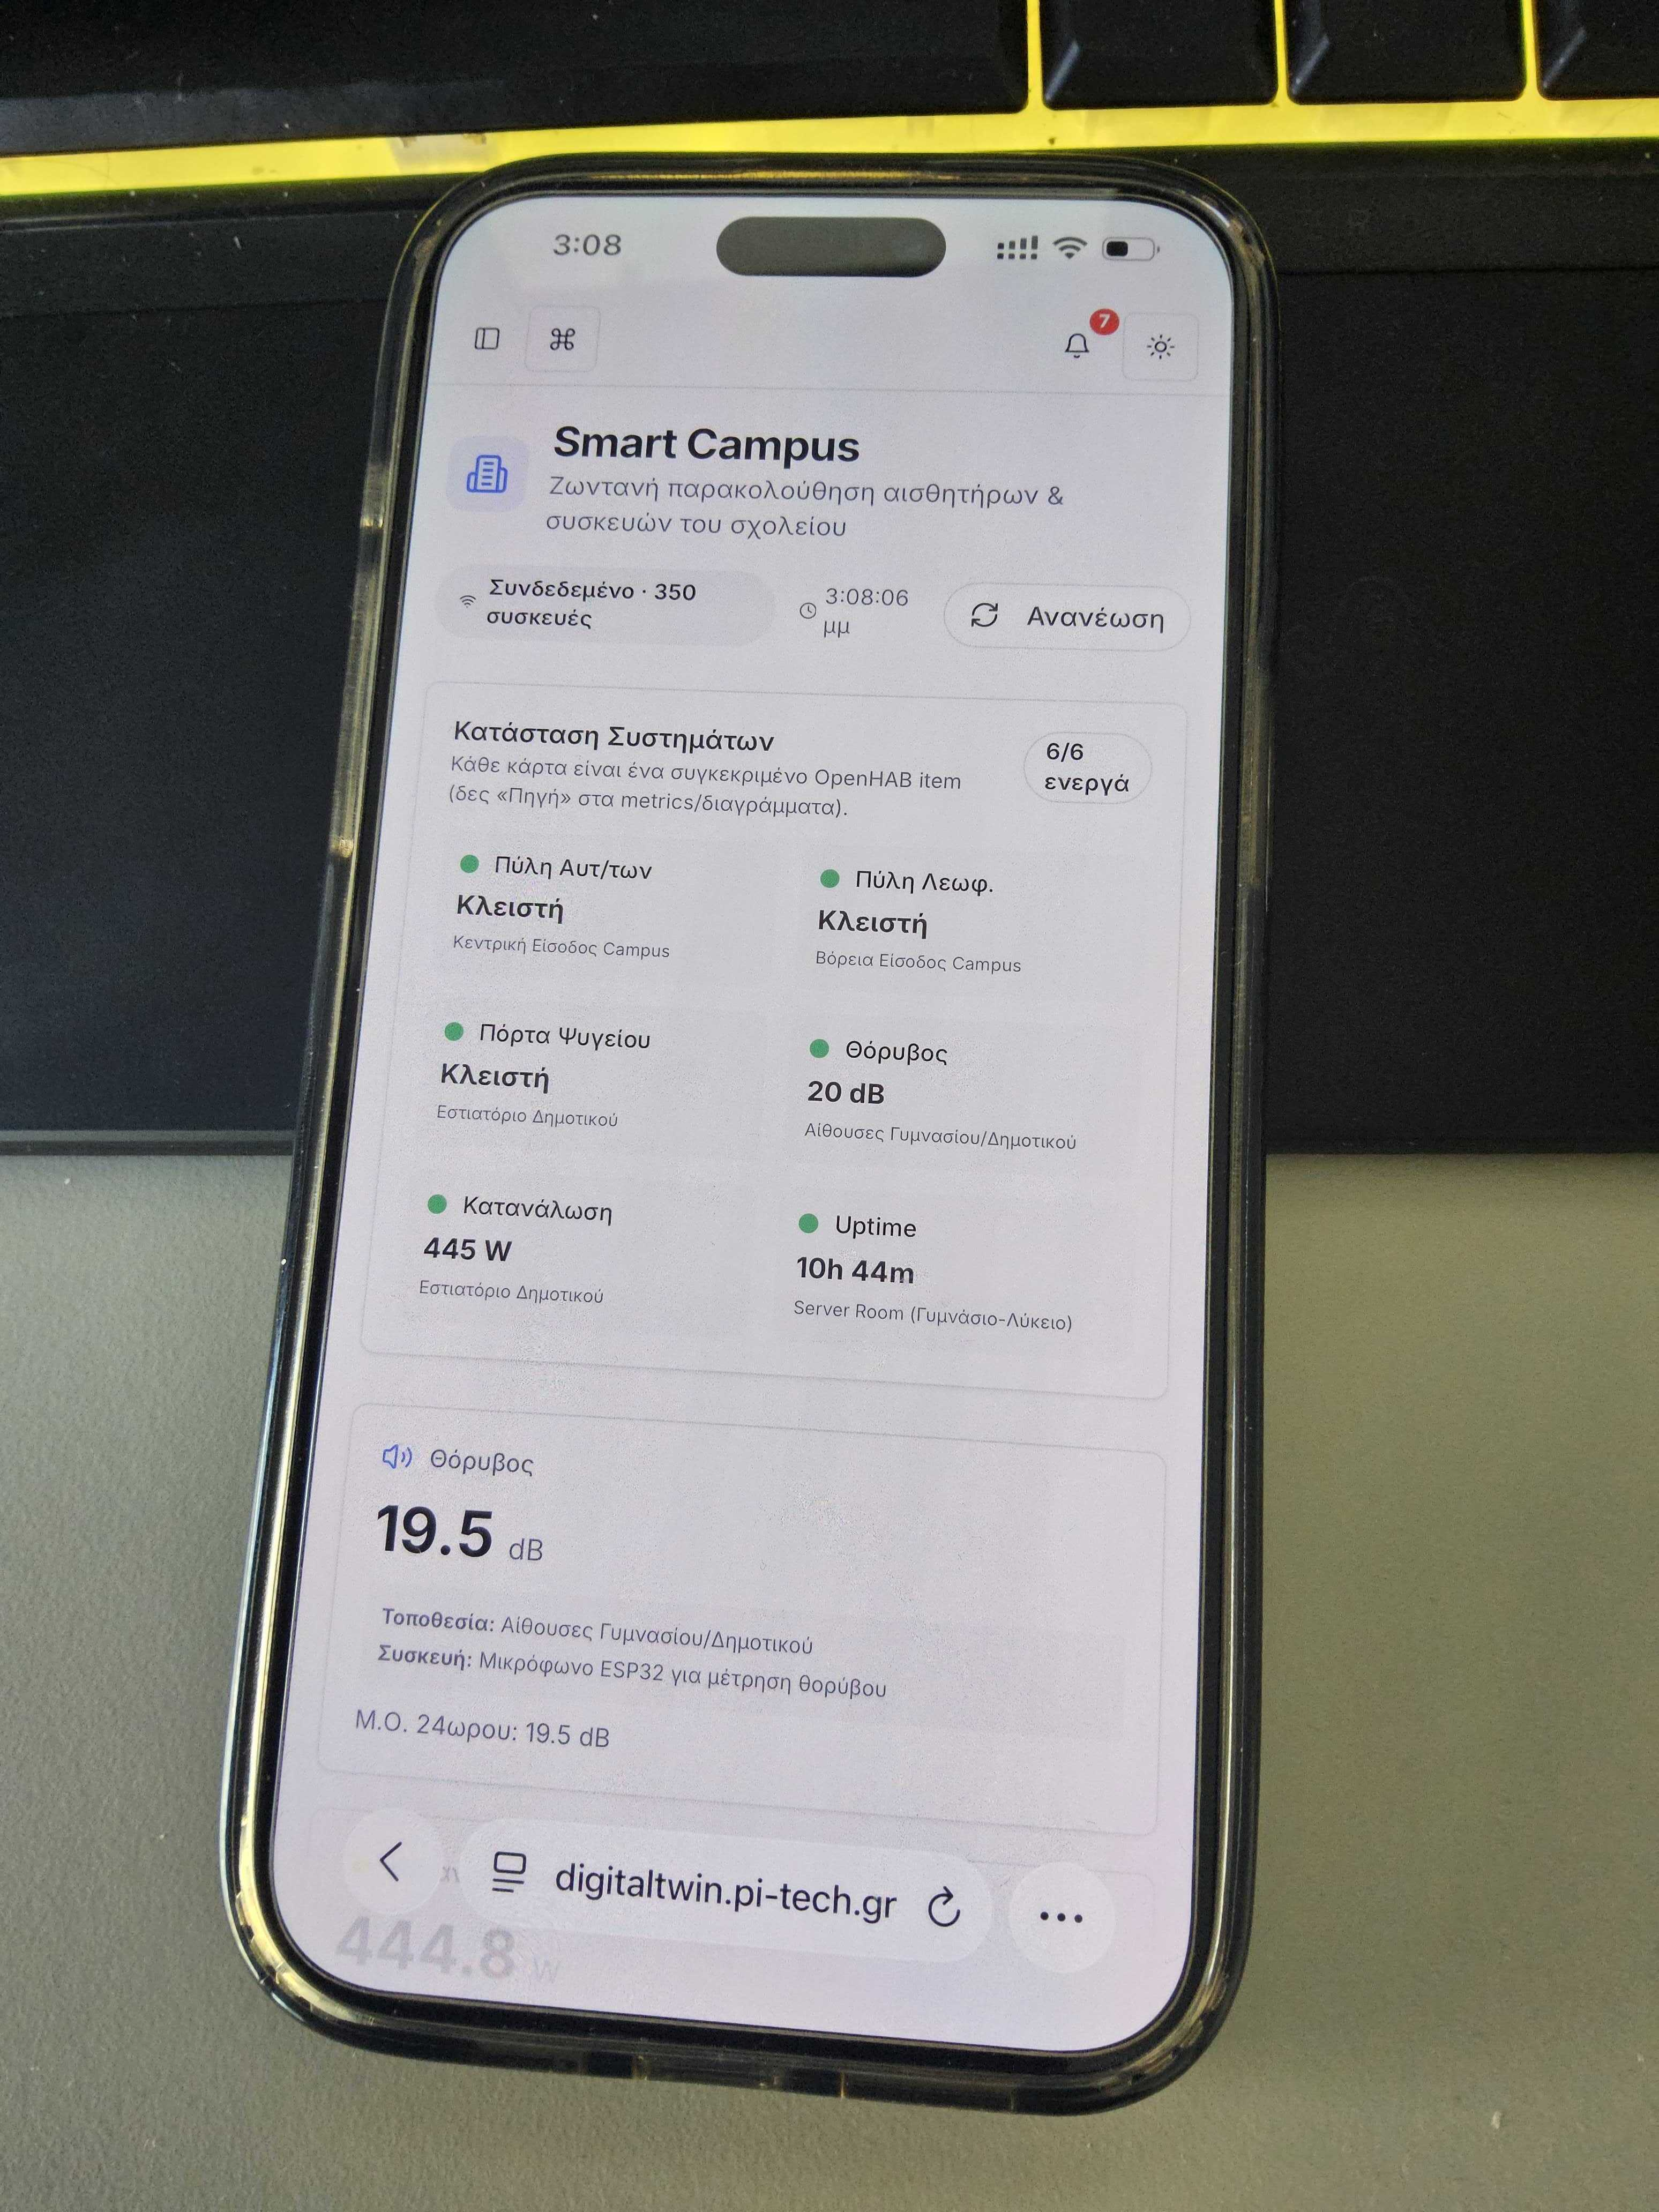
\includegraphics[width=0.31\textwidth]{fig_4_41}\hfill
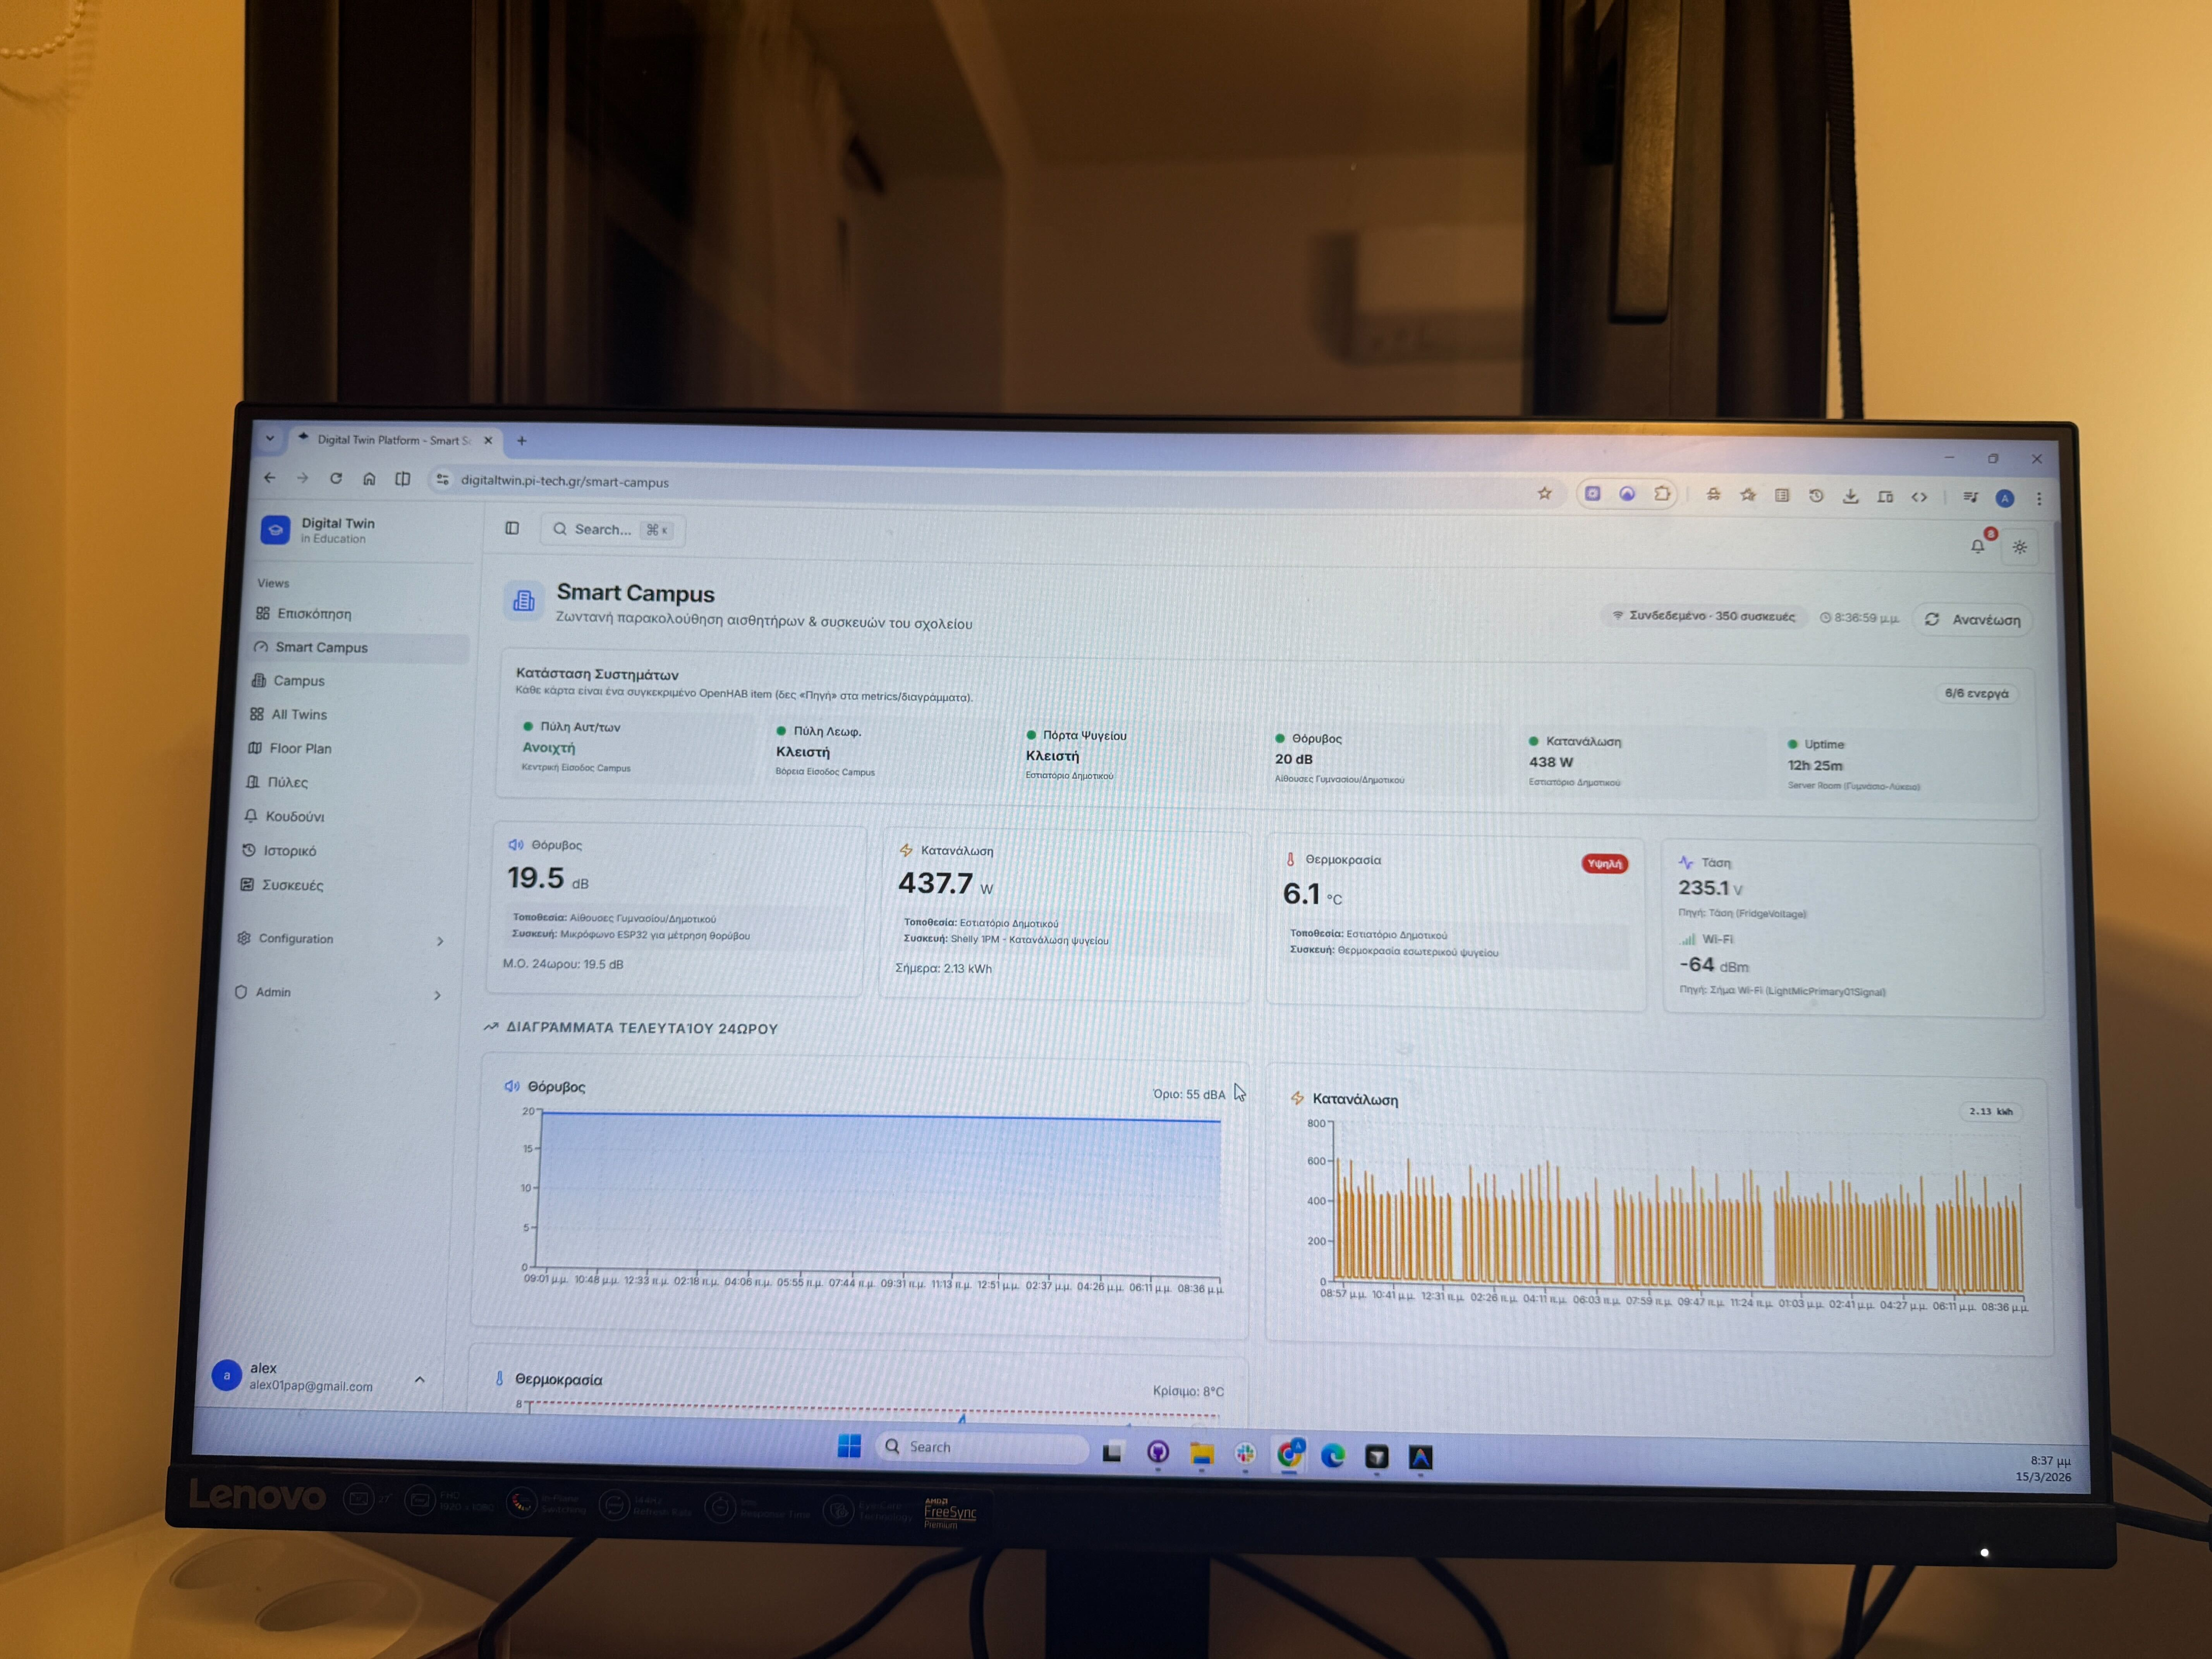
\includegraphics[width=0.31\textwidth]{fig_4_42}
\caption{Απεικόνιση της \textlatin{responsive} συμπεριφοράς της πλατφόρμας σε κινητές και φορητές συσκευές.}
\label{fig:responsive_views}
\end{figure}

\section{Συνολική Τεχνική Αποτίμηση του Κεφαλαίου}
Το παρόν κεφάλαιο περιέγραψε τη μετάβαση από το τοπικό πρωτότυπο με \textlatin{MQTT}, \textlatin{openHAB}, \textlatin{InfluxDB} και \textlatin{Grafana} σε μια πολυεπίπεδη αρχιτεκτονική \textlatin{cloud SaaS} με \textlatin{React}, \textlatin{Supabase/PostgreSQL} και \textlatin{Edge Functions}. Η τελική υλοποίηση συνδυάζει \textlatin{edge} συλλογή δεδομένων, σημασιολογική οργάνωση, αμφίδρομο έλεγχο, χωρική οπτικοποίηση \textlatin{2D/3D}, διαβαθμισμένη πρόσβαση και εξειδικευμένα widgets λειτουργικής ανάλυσης. Από αρχιτεκτονική άποψη, το σύστημα διαχωρίζει το επίπεδο πεδίου από το επίπεδο υπηρεσιών και διεπαφής, ώστε να υποστηρίζεται κλιμάκωση, απομακρυσμένη πρόσβαση και επέκταση σε πρόσθετα υποσυστήματα του σχολικού συγκροτήματος.

Η τελική μορφή της πλατφόρμας είναι επιχειρησιακά ενεργή στη διεύθυνση \href{https://digitaltwin.pi-tech.gr}{\textlatin{digitaltwin.pi-tech.gr}}. Η πρόσβαση στα πραγματικά δεδομένα της εγκατάστασης παρέχεται αποκλειστικά σε εξουσιοδοτημένους χρήστες μέσω διαπιστευτηρίων. Παράλληλα, διατίθεται \textlatin{Demo} περιβάλλον με προσομοιωμένα δεδομένα και πλήρη διαδραστικότητα --- συμπεριλαμβανομένου του ελέγχου πυλών και της \textlatin{quiet-lamp} --- το οποίο είναι προσβάσιμο μέσω του κουμπιού \textlatin{'Demo Sign In'} στη σελίδα εισόδου, χωρίς να απαιτούνται διαπιστευτήρια. Το \textlatin{Demo} περιβάλλον επιτρέπει την αξιολόγηση της πλατφόρμας και την κατανόηση του κύκλου \textlatin{Sense--Decide--Act} χωρίς πρόσβαση σε πραγματικά δεδομένα ή συσκευές.


\chapter{Μεθοδολογία Αξιολόγησης}

\section{Εισαγωγή στη Μεθοδολογία}
Η αξιολόγηση της αναπτυχθείσας πλατφόρμας σχεδιάστηκε με στόχο να τεκμηριωθεί τόσο η τεχνική της αποτελεσματικότητα όσο και η πρακτική της αξία σε πραγματικό σχολικό περιβάλλον. Η μεθοδολογία εφαρμόστηκε στο πεδίο μελέτης των Εκπαιδευτηρίων Πλάτων και οργανώθηκε γύρω από τρεις διακριτούς, αλλά αλληλοσυμπληρούμενους, άξονες: (α) την αξιολόγηση του μαθησιακού περιβάλλοντος μέσω της ακουστικής άνεσης, (β) την αξιολόγηση της ενεργειακής απόδοσης με κανονικοποίηση των καταναλώσεων σε \textlatin{kWh}/ημέρα, και (γ) την τεχνοοικονομική αξιολόγηση της επένδυσης με χρήση δεικτών \textlatin{CAPEX}, \textlatin{OPEX savings} και πενταετούς \textlatin{ROI}.

Η μεθοδολογική προσέγγιση ακολούθησε δύο διαδοχικά στάδια υλοποίησης. Στο πρώτο στάδιο, το οποίο αντιστοιχεί στο τοπικό πρωτότυπο (\textlatin{Minimum Viable Product - MVP}), η συλλογή του \textlatin{baseline} και των πρώτων τηλεμετρικών δεδομένων πραγματοποιήθηκε μέσω της υποδομής \textlatin{openHAB}/\textlatin{InfluxDB} στο φυσικό πεδίο. Το στάδιο αυτό επέτρεψε την αρχική επικύρωση των αισθητήρων, των κανόνων ελέγχου και της ροής δεδομένων από το επίπεδο των συσκευών προς το επίπεδο εποπτείας. Στο δεύτερο στάδιο, η πλήρης αναλυτική επεξεργασία, οι προβολές εξοικονόμησης, οι τεχνοοικονομικοί δείκτες και τα εργαλεία \textlatin{AI Energy Forecasting} ενσωματώθηκαν στη νέα \textlatin{Enterprise Cloud SaaS} πλατφόρμα, η οποία παρείχε πιο ώριμο περιβάλλον ανάλυσης, ιστορικής σύγκρισης και λήψης αποφάσεων για τον τελικό χρήστη.

Η παραπάνω διάκριση είναι ουσιώδης για την ερμηνεία των αποτελεσμάτων. Το τοπικό \textlatin{MVP} λειτούργησε ως πλαίσιο επιχειρησιακής μέτρησης και αρχικής απόδειξης σκοπιμότητας, ενώ η μετέπειτα \textlatin{SaaS} υλοποίηση μετέφερε την αξιολόγηση σε ένα ανώτερο επίπεδο, όπου η συσχέτιση δεδομένων, η εξαγωγή δεικτών απόδοσης και η προβολή οικονομικών ωφελειών μπορούσαν να εκτελούνται με περισσότερο τυποποιημένο και επεκτάσιμο τρόπο.

Η διασφάλιση της ποιότητας των μετρήσεων αποτέλεσε αναπόσπαστο μέρος της μεθοδολογίας. Πριν την έναρξη της συλλογής δεδομένων, πραγματοποιήθηκε βαθμονόμηση όλων των αισθητήρων έναντι πιστοποιημένων οργάνων αναφοράς. Ειδικότερα, οι κόμβοι ακουστικής παρακολούθησης (\textlatin{ESP32/INMP441}) βαθμονομήθηκαν έναντι βιομηχανικού ηχομέτρου, επιτυγχάνοντας ακρίβεια ±2 \textlatin{dBA}. Οι αισθητήρες θερμοκρασίας και υγρασίας (\textlatin{DHT22}) βαθμονομήθηκαν με αποτέλεσμα ακρίβεια ±0.5°C και ±2\% \textlatin{RH} αντίστοιχα. Η συνεχής παρακολούθηση της ποιότητας δεδομένων μέσω αυτοματοποιημένων ρουτινών ανίχνευσης εκτός ορίων (\textlatin{out-of-range detection}) διασφάλισε \textlatin{data quality score} 98.5\% καθ' όλη την περίοδο αξιολόγησης.

\section{Αξιολόγηση Μαθησιακού Περιβάλλοντος (Ακουστική Άνεση)}
Η αξιολόγηση του μαθησιακού περιβάλλοντος βασίστηκε στην παρακολούθηση της ακουστικής συμπεριφοράς των αιθουσών διδασκαλίας, με έμφαση στη λειτουργική επίδραση του κλειστού βρόχου ελέγχου στο επίπεδο θορύβου. Ως επιχειρησιακό κατώφλι παρέμβασης ορίστηκε η τιμή των 55 \textlatin{dBA} (\textlatin{LAeq}) κατά τη διάρκεια ενεργού διδακτικής ώρας. Η τιμή αυτή δεν αποτελεί θεσμοθετημένο όριο για ενεργή τάξη, αλλά επιλέχθηκε ως επιχειρησιακός συμβιβασμός μεταξύ της τιμής αναφοράς \textlatin{WHO} για άδεια αίθουσα ($\leq$35 \textlatin{dBA}) \cite{WHO1999, Kephalopoulos2015} και της πρακτικής ακουστικής δυναμικής κατά τη διδασκαλία, σύμφωνα με τη μεθοδολογία παθητικής αυτορρύθμισης συμπεριφοράς (\textlatin{behavioral nudging}) που προτείνεται στη βιβλιογραφία \cite{MogasRecalde2021}.

Στην πρώτη φάση αξιολόγησης, το σύστημα λειτουργούσε ως παθητικός παρατηρητής, καταγράφοντας το πλήθος και τη συχνότητα των υπερβάσεων του ορίου χωρίς να παράγει φυσική παρέμβαση στον χώρο. Η περίοδος αυτή παρείχε το σημείο αναφοράς για την κατανόηση της βασικής ακουστικής συμπεριφοράς των αιθουσών. Στη δεύτερη φάση, ενεργοποιήθηκε ο αμφίδρομος έλεγχος, κατά τον οποίο οι συνεχείς υπερβάσεις του ορίου οδηγούσαν στην ενεργοποίηση της διακριτικής οπτικής ένδειξης (\textlatin{quiet-lamp}). Με τον τρόπο αυτό, το σύστημα δεν περιοριζόταν στην καταγραφή, αλλά παρήγαγε μια ήπια μορφή ανατροφοδότησης που μπορούσε να επηρεάσει θετικά τη συμπεριφορά των μαθητών και τη συνολική λειτουργία της τάξης.

Η αξιολόγηση δεν στηρίχθηκε μόνο στην παρατήρηση μεμονωμένων μετρήσεων, αλλά στο πλήθος των υπερβάσεων ανά διδακτική περίοδο, στη χρονική διάρκειά τους και στη συγκριτική αποτίμηση των δύο φάσεων λειτουργίας. Οι παράμετροι και τα όρια που χρησιμοποιήθηκαν για την ακουστική αξιολόγηση συνοψίζονται στον Πίνακα~\ref{tab:noise_limits}. Η αρχική συλλογή των δεδομένων πραγματοποιήθηκε στο τοπικό \textlatin{MVP}, ενώ η μεταγενέστερη ανάλυση τάσεων και η οπτικοποίηση των αποτελεσμάτων μεταφέρθηκαν στο περιβάλλον της \textlatin{Cloud SaaS} πλατφόρμας, όπου μπορούσαν να παραχθούν συγκεντρωτικοί δείκτες και περισσότερο φιλικές προς τον τελικό χρήστη αναφορές.

\begin{table}[htbp]
\centering
\caption{Όρια θορύβου και παράμετροι ενεργοποίησης οπτικής ένδειξης}
\label{tab:noise_limits}
\begin{tabular}{|p{4.8cm}|p{3cm}|p{6.2cm}|}
\hline
\textbf{Παράμετρος} & \textbf{Τιμή} & \textbf{Ρόλος / Περιγραφή} \\
\hline
Συνιστώμενο επίπεδο υποβάθρου (Άδεια τάξη) & $\leq$ 35 \textlatin{dBA} & Τιμή αναφοράς για ήσυχο σχολικό περιβάλλον χωρίς ενεργή διδασκαλία. \\
\hline
Όριο ενεργοποίησης ένδειξης (Κατά τη διδασκαλία) & 55 \textlatin{dBA} & Επιχειρησιακό κατώφλι παρέμβασης για την ενεργοποίηση της οπτικής ανατροφοδότησης κατά την ενεργή διδακτική ώρα. \\
\hline
Χρονικό παράθυρο επιβεβαίωσης (\textlatin{Dwell Time}) & 20 δευτερόλεπτα & Συνεχής υπέρβαση του ορίου για το ελάχιστο αυτό διάστημα απαιτείται πριν ενεργοποιηθεί η ένδειξη, ώστε να αποφεύγονται στιγμιαίες ψευδο-ενεργοποιήσεις. \\
\hline
Περίοδος εφαρμογής & Ενεργή διδακτική ώρα & Ο κανόνας ελέγχου εφαρμόζεται μόνο στη διάρκεια μαθήματος και όχι σε διαλείμματα ή εκτός ωρολογίου προγράμματος. \\
\hline
Ενεργοποιητής (\textlatin{Actuator}) & Οπτική λυχνία (\textlatin{quiet-lamp}) & Μη παρεμβατικός μηχανισμός ανατροφοδότησης που στοχεύει στην ήπια αυτορρύθμιση της συμπεριφοράς των μαθητών. \\
\hline
\end{tabular}
\end{table}

\section{Μεθοδολογία Ενεργειακής Αξιολόγησης}
Η αξιολόγηση της ενεργειακής επίδρασης της πλατφόρμας βασίστηκε στη σύγκριση της κατανάλωσης ηλεκτρικής ενέργειας πριν και μετά την επιχειρησιακή εφαρμογή του ψηφιακού διδύμου. Ως πρωτογενές υλικό χρησιμοποιήθηκαν οι επίσημοι λογαριασμοί ηλεκτρικής ενέργειας της εγκατάστασης για την περίοδο από τον Σεπτέμβριο του 2024 έως τον Νοέμβριο του 2025. Επειδή οι επιμέρους περίοδοι τιμολόγησης δεν είχαν σταθερή διάρκεια σε ημέρες, η σύγκριση δεν θα μπορούσε να γίνει αξιόπιστα σε επίπεδο απόλυτων μηνιαίων τιμών. Για τον λόγο αυτό εφαρμόστηκε κανονικοποίηση των καταναλώσεων σε \textlatin{kWh}/ημέρα, καθώς οι περίοδοι τιμολόγησης κυμαίνονταν μεταξύ 28 και 63 ημερών, καθιστώντας αδύνατη την άμεση σύγκριση απόλυτων τιμών, ώστε να προκύψει μια συγκρίσιμη και μεθοδολογικά ομοιογενής βάση αξιολόγησης.

Η ενεργειακή μεθοδολογία υλοποιήθηκε επίσης σε δύο στάδια. Στο πρώτο στάδιο, το τοπικό \textlatin{MVP} κατέγραψε το \textlatin{baseline} της εγκατάστασης και τα πρώτα επιχειρησιακά δεδομένα μέσω της σύζευξης \textlatin{openHAB}, \textlatin{MQTT} και \textlatin{InfluxDB}. Το στάδιο αυτό λειτούργησε ως σημείο αναφοράς για τη συμπεριφορά της εγκατάστασης πριν από την πλήρη ωρίμανση των αυτοματισμών. Στο δεύτερο στάδιο, τα ιστορικά δεδομένα και οι λογικές ελέγχου μεταφέρθηκαν στη νέα \textlatin{Enterprise Cloud SaaS} πλατφόρμα, όπου κατέστη δυνατή η ενοποιημένη ανάλυση χρονοσειρών, η σύγκριση \textlatin{baseline} και βελτιστοποιημένης λειτουργίας, καθώς και η παραγωγή προβλέψεων μέσω \textlatin{AI Energy Forecasting}.

Για την ερμηνεία των αποτελεσμάτων διαχωρίστηκαν δύο επίπεδα σύγκρισης. Το πρώτο αφορά τη γενική ακατέργαστη σύγκριση (\textlatin{raw comparison}) του συνόλου των διαθέσιμων περιόδων πριν και μετά. Το δεύτερο αφορά τη σύγκριση της περιόδου βάσης (\textlatin{baseline}) με την περίοδο πλήρους επιχειρησιακής βελτιστοποίησης, κατά την οποία οι κανόνες ελέγχου είχαν ενεργοποιηθεί σταθερά και η πλατφόρμα λειτουργούσε με ώριμο τρόπο. Η δεύτερη προσέγγιση χρησιμοποιήθηκε ως κύριο λειτουργικό \textlatin{KPI}, καθώς αντανακλά με μεγαλύτερη πιστότητα την απόδοση του συστήματος υπό συνθήκες πλήρους λειτουργίας.

Η νέα \textlatin{Cloud SaaS} πλατφόρμα επέτρεψε, επιπλέον, την ενσωμάτωση αναλυτικών εργαλείων πρόβλεψης κόστους και μελλοντικής κατανάλωσης. Η δυνατότητα αυτή δεν αναιρεί τη μεθοδολογία της αρχικής συλλογής, αλλά τη συμπληρώνει, παρέχοντας ένα πιο ώριμο περιβάλλον αξιολόγησης για διοικητικούς και τεχνικούς χρήστες, με καλύτερη αναγνωσιμότητα και μεγαλύτερη επιχειρησιακή αξία.

\section{\texorpdfstring{Τεχνοοικονομική Μεθοδολογία (Υπολογισμός \textlatin{ROI})}{Τεχνοοικονομική Μεθοδολογία (Υπολογισμός ROI)}}
Η τεχνοοικονομική αξιολόγηση σχεδιάστηκε με στόχο να εκτιμηθεί κατά πόσο η αναπτυχθείσα πλατφόρμα μπορεί να υποστηρίξει μια βιώσιμη επένδυση για ένα σχολικό συγκρότημα. Η ανάλυση στηρίχθηκε στη σύγκριση του αρχικού κόστους κεφαλαίου (\textlatin{CAPEX}) με τα αναμενόμενα ετήσια λειτουργικά οφέλη (\textlatin{OPEX savings}), λαμβάνοντας υπόψη τόσο τη μείωση της κατανάλωσης ηλεκτρικής ενέργειας όσο και την αποφυγή κόστους που συνδέεται με συμβάντα λειτουργικής αστοχίας και συντήρησης του εξοπλισμού ψύξης.

Το \textlatin{CAPEX} περιλαμβάνει το κόστος του υλικού εξοπλισμού, της εγκατάστασης, της παραμετροποίησης, της ολοκλήρωσης των επιμέρους υποσυστημάτων και της ανάπτυξης του λογισμικού που απαιτήθηκε για την επιχειρησιακή ωρίμανση της πλατφόρμας. Τα \textlatin{OPEX savings} εκτιμώνται με βάση τη μείωση της κατανάλωσης ενέργειας, χρησιμοποιώντας σταθερή τιμή αναφοράς 0{,}162~\euro/\textlatin{kWh}, βάσει των επίσημων λογαριασμών ηλεκτρικής ενέργειας της περιόδου αξιολόγησης, καθώς και με βάση τη μείωση των απωλειών που σχετίζονται με δυσλειτουργίες του εξοπλισμού και επαναλαμβανόμενα συμβάντα μη αποδοτικής λειτουργίας.

Σε αντίθεση με το τοπικό \textlatin{MVP}, το οποίο εξυπηρετούσε κυρίως τη συλλογή και την αρχική επιβεβαίωση της μεθοδολογίας, η \textlatin{Enterprise Cloud SaaS} πλατφόρμα παρείχε το κατάλληλο περιβάλλον για την παραγωγή προβολών \textlatin{ROI}, την απεικόνιση των ταμειακών ροών και τη διαμόρφωση ευανάγνωστων αναφορών προς τον τελικό χρήστη. Στο ίδιο πλαίσιο εντάχθηκε και η χρήση \textlatin{AI Energy Forecasting}, η οποία επέτρεψε την υποστήριξη προβλεπτικών σεναρίων και την ενίσχυση της λήψης αποφάσεων σε τεχνικό και διοικητικό επίπεδο.

Η τελική αξιολόγηση στηρίχθηκε σε δείκτες όπως ο χρόνος απόσβεσης (\textlatin{Payback Period}) και η πενταετής απόδοση επένδυσης (\textlatin{5-year ROI}), ώστε η αποτελεσματικότητα της πλατφόρμας να τεκμηριωθεί όχι μόνο σε τεχνικό αλλά και σε επιχειρησιακό επίπεδο. Με τον τρόπο αυτό, η μεθοδολογία του κεφαλαίου συνδέει άμεσα τη μετρητική διάσταση του ψηφιακού διδύμου με την πρακτική αξιοποίησή του ως εργαλείο βελτιστοποίησης και στρατηγικού σχεδιασμού. Το Σχήμα~\ref{fig:methodology_flow} παρουσιάζει το συνολικό διάγραμμα ροής της μεθοδολογίας αξιολόγησης.

\begin{figure}[htbp]
\centering
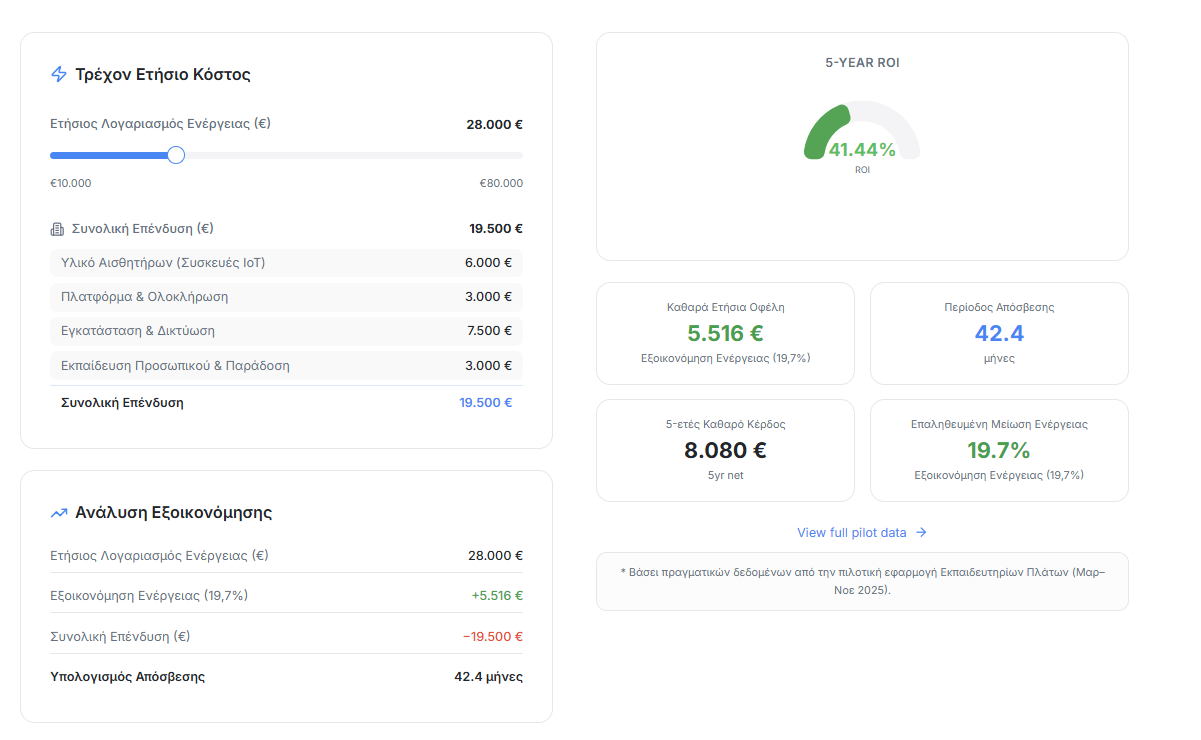
\includegraphics[width=\textwidth]{fig_5_1}
\caption{Διάγραμμα ροής της μεθοδολογίας αξιολόγησης και ενδεικτική απεικόνιση του περιβάλλοντος τεχνοοικονομικής ανάλυσης}
\label{fig:methodology_flow}
\end{figure}





\chapter{Αποτελέσματα και Ανάλυση Δεδομένων}

\section{Αποτελέσματα Ακουστικής Άνεσης στο Μαθησιακό Περιβάλλον}
Η εφαρμογή του Ψηφιακού Διδύμου επέφερε άμεσα και μετρήσιμα αποτελέσματα ως προς την Ποιότητα Εσωτερικού Περιβάλλοντος (\textlatin{IEQ}). Η συλλογή των αρχικών τηλεμετρικών δεδομένων για τον θόρυβο πραγματοποιήθηκε κατά τη φάση του τοπικού \textlatin{MVP}, μέσω της σύζευξης \textlatin{ESP32}, \textlatin{MQTT}, \textlatin{openHAB} και \textlatin{InfluxDB}, η οποία επέτρεψε την αξιόπιστη αποτύπωση των υπερβάσεων του επιχειρησιακού ορίου των 55 \textlatin{dBA}. Στη συνέχεια, η νέα \textlatin{Enterprise Cloud SaaS} πλατφόρμα αξιοποιήθηκε για την ενοποιημένη ανάλυση, την πιο φιλική οπτικοποίηση και την ευανάγνωστη παρουσίαση των αποτελεσμάτων προς τεχνικούς και διοικητικούς χρήστες.

Η χρήση του κλειστού βρόχου ελέγχου για τη διατήρηση του θορύβου κάτω από το δυναμικό όριο των 55 \textlatin{dBA} αποδείχθηκε ιδιαίτερα αποτελεσματική. Σε αντίθεση με τη χρήση ηχητικών συναγερμών (\textlatin{buzzers}), η οποία θα διατάρασσε την εκπαιδευτική διαδικασία, η διακριτική οπτική ανατροφοδότηση (\textlatin{quiet-lamp}) λειτούργησε ομαλά ως μηχανισμός αυτορρύθμισης της συμπεριφοράς των μαθητών. Τα αρχικά δεδομένα από την υποδομή παρακολούθησης και η μεταγενέστερη ενοποιημένη απεικόνισή τους στο \textlatin{cloud} περιβάλλον, όπως αποτυπώνεται στο Σχήμα~\ref{fig:noise_results}, κατέδειξαν σημαντική μείωση στον αριθμό των ημερήσιων υπερβάσεων του ορίου, συμβάλλοντας στη διαμόρφωση περιβάλλοντος περισσότερο συμβατού με τις κατευθυντήριες οδηγίες ακουστικής άνεσης.

\begin{figure}[htbp]
\centering
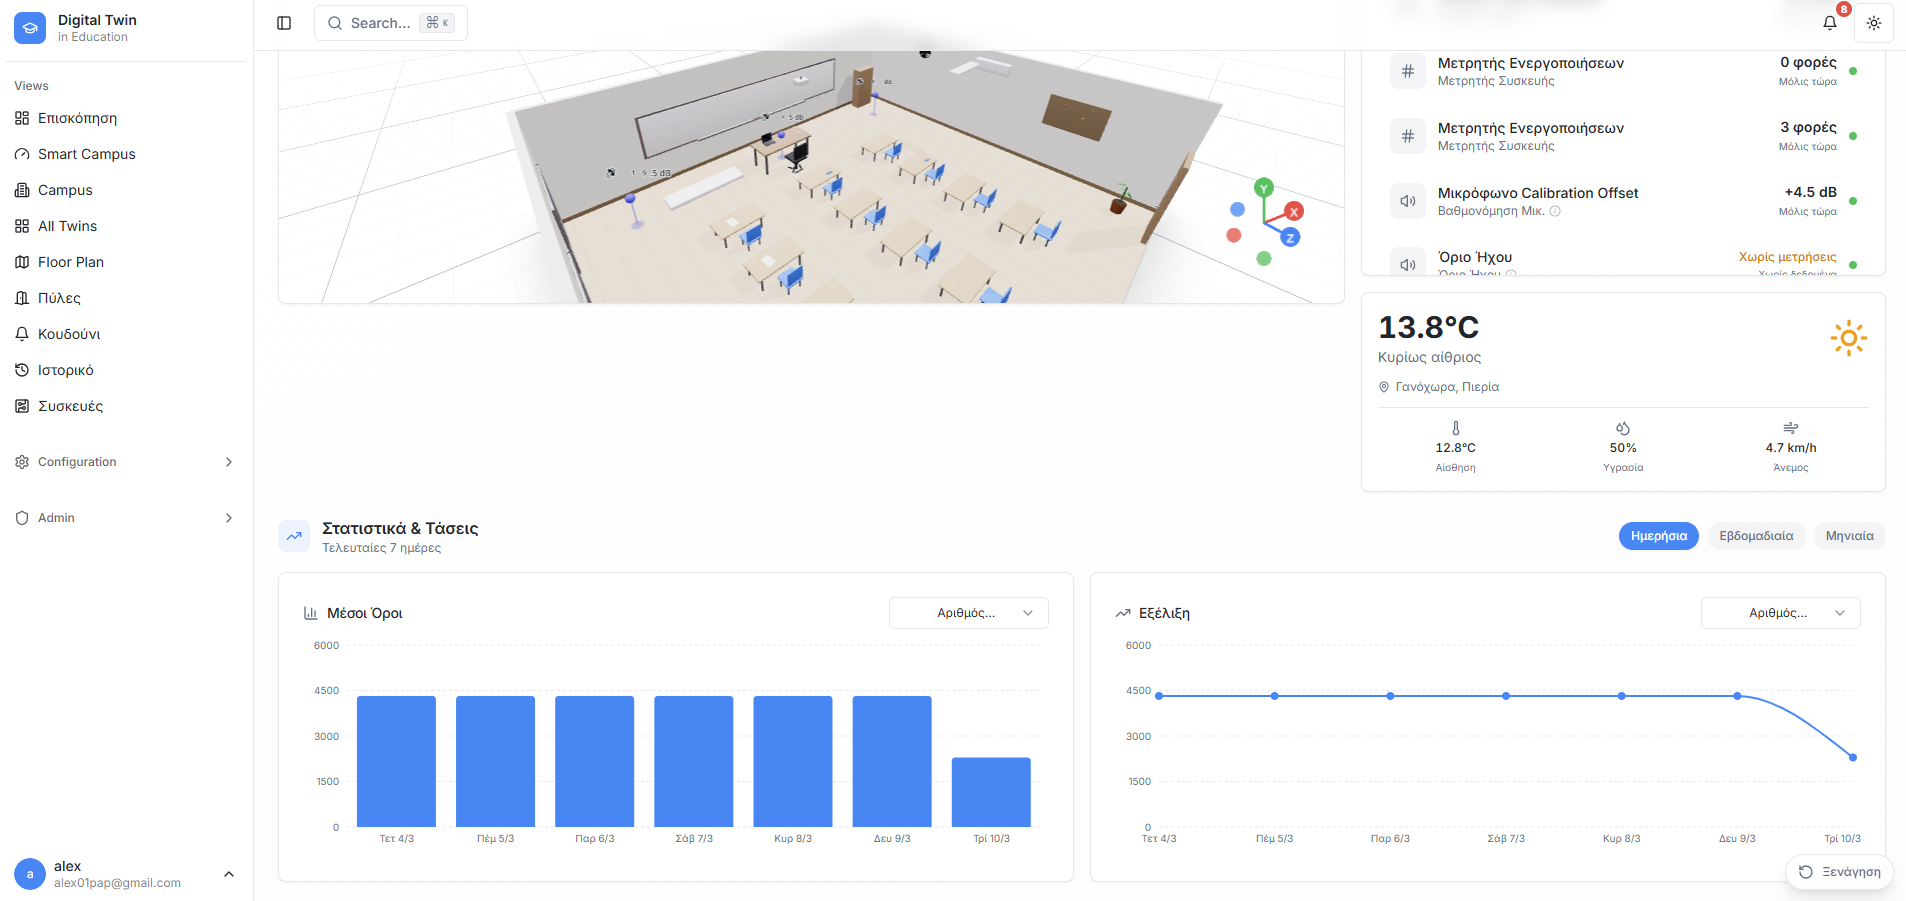
\includegraphics[width=\textwidth]{fig_6_1}
\caption{Απεικόνιση επιπέδων θορύβου και υπερβάσεων (\textlatin{exceedances}) εντός της σχολικής αίθουσας}
\label{fig:noise_results}
\end{figure}

Αναφορικά με την ακρίβεια των αισθητήρων, οι κόμβοι \textlatin{ESP32/INMP441} επαληθεύτηκαν έναντι πιστοποιημένου βιομηχανικού ηχομέτρου αναφοράς, επιτυγχάνοντας μέση ακρίβεια ±2 \textlatin{dBA}. Αντίστοιχα, οι αισθητήρες \textlatin{DHT22} για θερμοκρασία και υγρασία επιβεβαιώθηκαν με ακρίβεια ±0.5°C και ±2\% \textlatin{RH} αντίστοιχα μετά από βαθμονόμηση. Η συνολική αξιοπιστία δεδομένων (\textlatin{data quality score}) του συστήματος ανήλθε σε 98.5\%, τιμή που υπολογίστηκε μέσω διασταύρωσης των μετρήσεων των αισθητήρων με ανεξάρτητα όργανα αναφοράς.

\section{Ανάλυση Ενεργειακής Απόδοσης και Σύγκριση Δεδομένων}
Για την αξιολόγηση της ενεργειακής επίδρασης της πλατφόρμας, πραγματοποιήθηκε σύγκριση της μέσης ημερήσιας κατανάλωσης (\textlatin{kWh}/ημέρα) μεταξύ της περιόδου πριν και μετά την εφαρμογή του Ψηφιακού Διδύμου. Η χρήση της ημερήσιας κατανάλωσης κρίθηκε απαραίτητη για τη διασφάλιση μιας δίκαιης σύγκρισης, καθώς οι περίοδοι τιμολόγησης των λογαριασμών ρεύματος διέφεραν σε πλήθος ημερών.

Από πλευράς αρχιτεκτονικής ροής δεδομένων, το \textlatin{baseline} και οι πρώτες ενεργειακές χρονοσειρές συγκεντρώθηκαν στο τοπικό \textlatin{MVP} μέσω της υποδομής \textlatin{openHAB}/\textlatin{InfluxDB}. Η ίδια τηλεμετρία, αφού ωρίμασε λειτουργικά και εμπλουτίστηκε με μεγαλύτερο χρονικό ορίζοντα παρατήρησης, μεταφέρθηκε στο περιβάλλον της \textlatin{Enterprise Cloud SaaS} πλατφόρμας, όπου κατέστη δυνατή η ενοποιημένη ανάλυση, η συγκριτική εποπτεία \textlatin{baseline} και βελτιστοποιημένης λειτουργίας, καθώς και η παραγωγή προβολών μέσω \textlatin{AI Energy Forecasting} για τις μελλοντικές ταμειακές ροές και τους δείκτες \textlatin{ROI}.

\subsection{Συνολική Σύγκριση Ακατέργαστων Δεδομένων (\textlatin{Raw Comparison} -- 10,9\%)}
Η πρώτη ανάλυση αφορά το σύνολο των διαθέσιμων δεδομένων από τον Σεπτέμβριο του 2024 έως τον Νοέμβριο του 2025.
\begin{itemize}
\item \textbf{Περίοδος Πριν (Σεπ 2024 -- Φεβ 2025):} Η μέση ημερήσια κατανάλωση ανήλθε στις 201 \textlatin{kWh}/ημέρα.
\item \textbf{Περίοδος Μετά (Μάρ 2025 -- Νοέ 2025):} Η μέση ημερήσια κατανάλωση μειώθηκε στις 179 \textlatin{kWh}/ημέρα.
\end{itemize}
\textbf{Αποτέλεσμα:} Η ποσοστιαία μείωση ανέρχεται σε 10,9\%. Το νούμερο αυτό αντιπροσωπεύει τη γενική τάση εξοικονόμησης στο σύνολο του έτους, συμπεριλαμβανομένων περιόδων με χαμηλότερες απαιτήσεις θέρμανσης ή ψύξης. Η σύγκριση αυτή προκύπτει από το πλήρες σώμα των διαθέσιμων δεδομένων και αποτυπώνει την πρώτη, πιο συνολική ανάγνωση της ενεργειακής συμπεριφοράς πριν και μετά την ωρίμανση της λειτουργίας του συστήματος.
\begin{equation}
\Delta E_{\text{raw}} = \frac{201-179}{201}\cdot 100 = 10{,}9\%
\end{equation}

Αξίζει να σημειωθεί ότι ο Μάρτιος 2025, ο οποίος αντιστοιχεί στη φάση εγκατάστασης και βαθμονόμησης του συστήματος, εμφανίζει οριακή αύξηση κατανάλωσης (228 \textlatin{kWh}/ημέρα, +2,2\% \textlatin{vs baseline}). Αυτό αποδίδεται στη φυσική παρουσία τεχνικών στο πεδίο, στις δοκιμαστικές λειτουργίες εξοπλισμού και στο γεγονός ότι οι κανόνες αυτοματισμού δεν είχαν ακόμη ενεργοποιηθεί πλήρως — το σύστημα λειτουργούσε αποκλειστικά ως παθητικός παρατηρητής (\textlatin{Digital Shadow}). Η επιβεβαίωση αυτής της ερμηνείας προκύπτει άμεσα από τα δεδομένα του Απριλίου 2025, όπου μόλις ενεργοποιήθηκαν οι αυτοματισμοί, η κατανάλωση έπεσε αμέσως στις 190 \textlatin{kWh}/ημέρα (-14,8\%), αποτυπώνοντας την ομαλή καμπύλη βελτιστοποίησης που χαρακτηρίζει ένα σύστημα \textlatin{IoT} κατά τη φάση λειτουργικής ωρίμανσής του.

\subsection{Σύγκριση Περιόδου Βελτιστοποίησης (\textlatin{Weighted/Baseline Comparison} -- 19,7\%)}
Για μια βαθύτερη κατανόηση της απόδοσης του συστήματος, ορίστηκε μια Περίοδος Βάσης (\textlatin{Baseline}) που περιλαμβάνει τους μήνες αιχμής πριν την εφαρμογή του διδύμου, και μια Περίοδος Βελτιστοποίησης.
\begin{itemize}
\item \textbf{Σταθμισμένο \textlatin{Baseline}:} Λαμβάνοντας υπόψη τους μήνες με πλήρη λειτουργία του σχολείου, η κατανάλωση αναφοράς ορίστηκε στις 223 \textlatin{kWh}/ημέρα.
\item \textbf{Περίοδος Βελτιστοποίησης:} Με την πλήρη ενεργοποίηση των κανόνων του Ψηφιακού Διδύμου (όπως ο \texttt{FridgeGuardian} και η διαχείριση φωτισμού), η κατανάλωση σταθεροποιήθηκε στις 179 \textlatin{kWh}/ημέρα.
\end{itemize}
\textbf{Αποτέλεσμα:} Η μείωση αυτή της τάξεως του 19,7\% τεκμηριώνει τη λειτουργική δυναμική του συστήματος όταν αυτό λειτουργεί σε πλήρη ισχύ και διαχειρίζεται ενεργά τα φορτία του κτιρίου. Πρόκειται για το βασικό λειτουργικό \textlatin{KPI} της ενεργειακής αξιολόγησης, το οποίο δεν περιορίζεται στη συλλογή των δεδομένων από το αρχικό \textlatin{MVP}, αλλά αναδεικνύεται με σαφέστερο και επιχειρησιακά χρησιμότερο τρόπο μέσω των εργαλείων ανάλυσης της \textlatin{Cloud SaaS} πλατφόρμας.
\begin{equation}
\Delta E_{\text{weighted}} = \frac{223-179}{223}\cdot 100 = 19{,}7\%
\end{equation}

\subsection{\textlatin{Peak Performance}: Σύγκριση \textlatin{Year-over-Year} (32,5\%)}
Η πιο εντυπωσιακή απόδειξη της αξίας του Ψηφιακού Διδύμου προκύπτει από τη σύγκριση του Νοεμβρίου 2025 με τον Νοέμβριο 2024:
\begin{itemize}
\item \textbf{Νοέμβριος 2024:} 252 \textlatin{kWh}/ημέρα.
\item \textbf{Νοέμβριος 2025:} 170 \textlatin{kWh}/ημέρα.
\item \textbf{Μείωση:} 32,5\%.
\end{itemize}

Η ανάλυση των δεδομένων αναδεικνύει δύο διακριτές κορυφαίες επιδόσεις, κάθε μία με διαφορετική μεθοδολογική σημασία.

Ο Οκτώβριος 2025 αποτελεί τον μήνα με την κορυφαία απόδοση έναντι του γενικού \textlatin{Baseline}: με κατανάλωση 145 \textlatin{kWh}/ημέρα έναντι των 223 \textlatin{kWh}/ημέρα του σταθμισμένου μέσου όρου, καταγράφεται μείωση -35,0\%. Ο αριθμός αυτός αποτυπώνει την απόλυτη αποτελεσματικότητα του συστήματος κάτω από ιδανικές λειτουργικές συνθήκες.

Ο Νοέμβριος 2025 αποτελεί τον μήνα με την κορυφαία \textlatin{Year-over-Year (YoY)} απόδοση: με κατανάλωση 170 \textlatin{kWh}/ημέρα έναντι 252 \textlatin{kWh}/ημέρα τον Νοέμβριο 2024, καταγράφεται μείωση -32,5\%. Η σύγκριση αυτή έχει ιδιαίτερη ακαδημαϊκή αξία, διότι ελέγχει το σύστημα υπό παρόμοιες εποχιακές και λειτουργικές συνθήκες (ίδιος μήνας, ίδιο σχολικό πρόγραμμα, παρόμοιες καιρικές συνθήκες), απομονώνοντας έτσι την πραγματική επίδραση της πλατφόρμας από εποχιακές διακυμάνσεις. Πρόκειται για τον ισχυρότερο δείκτη αποτελεσματικότητας του Ψηφιακού Διδύμου κατά τους ενεργοβόρους χειμερινούς μήνες.
Η τάση αυτή είναι συμβατή με ευρωπαϊκά ευρήματα για ενεργειακή βελτιστοποίηση κτιρίων και δείκτες έξυπνης ετοιμότητας (\textlatin{SRI}) \cite{Apostolopoulos2022, Markoska2019, EUParliament2024, Fokaides2020, Zamanidou2024}. Τα συγκεντρωτικά ενεργειακά αποτελέσματα παρουσιάζονται στον Πίνακα~\ref{tab:energy_comparison}, ενώ η μηνιαία εξέλιξη της κατανάλωσης κατά την πιλοτική φάση αποτυπώνεται στον Πίνακα~\ref{tab:monthly_evolution}.

\begin{table}[htbp]
\centering
\caption{Συγκριτικός πίνακας ημερήσιας ενεργειακής κατανάλωσης Πριν και Μετά}
\label{tab:energy_comparison}
\begin{tabular}{|l|c|c|c|}
\hline
\textbf{Μετρική} & \textbf{Περίοδος \textlatin{Baseline}} & \textbf{Ψηφιακό Δίδυμο} & \textbf{Μεταβολή} \\
\hline
Περίοδος Μέτρησης & Σεπ. 2024 - Φεβ. 2025 & Μαρ. 2025 - Νοε. 2025 & - \\
\hline
Σύνολο Ημερών & 122 ημέρες & 226 ημέρες & - \\
\hline
Μέση Ημερήσια Κατανάλωση & \textbf{201 \textlatin{kWh}/ημέρα} & \textbf{179 \textlatin{kWh}/ημέρα} & \textbf{-10,9\%} \\
\hline
Σταθμισμένη Σύγκριση (\textlatin{Baseline}) & 223 \textlatin{kWh}/ημέρα & 179 \textlatin{kWh}/ημέρα & \textbf{-19,7\%} \\
\hline
Σύγκριση Νοεμβρίου (\textlatin{YoY}) & 252 \textlatin{kWh}/ημέρα & 170 \textlatin{kWh}/ημέρα & \textbf{-32,5\%} \\
\hline
\end{tabular}
\end{table}

Σημειώνεται ότι ο Πίνακας Β.2 του Παραρτήματος Β παρουσιάζει \textlatin{YoY} σύγκριση αποκλειστικά για τους μήνες Σεπτέμβριο--Νοέμβριο, καθώς αυτοί είναι οι μόνοι μήνες για τους οποίους υπάρχουν αντίστοιχα τιμολογημένα δεδομένα και στις δύο χρονιές (2024 και 2025). Οι μήνες Μάρτιος--Αύγουστος 2025 δεν διαθέτουν αντίστοιχο \textlatin{baseline} 2024 στα διαθέσιμα στοιχεία τιμολόγησης και επομένως εξαιρούνται από τη \textlatin{YoY} ανάλυση.

\begin{table}[htbp]
\centering
\caption{Μηνιαία εξέλιξη κατανάλωσης κατά τη διάρκεια της πιλοτικής εφαρμογής (Μάρ--Νοε 2025).}
\label{tab:monthly_evolution}
\begin{tabular}{|l|c|c|l|}
\hline
\textbf{Μήνας} & \textbf{\textlatin{kWh}/ημέρα} & \textbf{\textlatin{vs Baseline (223)}} & \textbf{Φάση Λειτουργίας} \\
\hline
Μάρτιος 2025 & 228 & +2,2\% & Εγκατάσταση \& Βαθμονόμηση \\
\hline
Απρίλιος 2025 & 190 & -14,8\% & Πρώτη Βελτιστοποίηση \\
\hline
Σεπτέμβριος 2025 & 197 & -11,7\% & Σταθερή Λειτουργία \\
\hline
Οκτώβριος 2025 & 145 & -35,0\% & Κορυφαία Απόδοση (\textlatin{vs Baseline}) \\
\hline
Νοέμβριος 2025 & 170 & -23,8\% & Κορυφαία Απόδοση (\textlatin{YoY: -32,5\%}) \\
\hline
\end{tabular}
\end{table}

\subsection*{Ερμηνεία \textlatin{YoY} Αυξήσεων (Σεπτέμβριος--Οκτώβριος)}
Στον Πίνακα Β.2 παρατηρείται ότι οι μήνες Σεπτέμβριος και Οκτώβριος 2025 εμφανίζουν \textlatin{YoY} αύξηση (+20,9\% και +8,2\% αντίστοιχα) σε σχέση με τους ίδιους μήνες του 2024. Η ερμηνεία αυτής της παρατήρησης απαιτεί διαχωρισμό των δύο μεθοδολογιών σύγκρισης.

Οι μήνες Σεπτέμβριος και Οκτώβριος 2024 παρουσίασαν ασυνήθιστα χαμηλή κατανάλωση (163 \textlatin{kWh}/ημέρα και 134 \textlatin{kWh}/ημέρα αντίστοιχα), σημαντικά κατώτερη από το σταθμισμένο \textlatin{baseline} (223 \textlatin{kWh}/ημέρα), πιθανώς λόγω ευνοϊκών καιρικών συνθηκών ή μειωμένης λειτουργίας κατά τις μεταβατικές εποχές. Συνεπώς, η \textlatin{YoY} αύξηση δεν αντανακλά μείωση αποδοτικότητας του συστήματος, αλλά απλώς υψηλότερη βάση σύγκρισης τους αντίστοιχους μήνες του 2025.

Αντίθετα, η σύγκριση έναντι του σταθμισμένου \textlatin{Baseline} επιβεβαιώνει ότι και οι δύο μήνες παρέμειναν κάτω από το επίπεδο αναφοράς (197 \textlatin{kWh}/ημέρα = -11,7\% και 145 \textlatin{kWh}/ημέρα = -35,0\% αντίστοιχα), τεκμηριώνοντας τη σταθερή αποτελεσματικότητα της πλατφόρμας. Για τον λόγο αυτό, ο κύριος δείκτης αξιολόγησης της παρούσας μελέτης (\textlatin{KPI}) παραμένει η σύγκριση \textlatin{vs Baseline} (-19,7\%), η οποία είναι ανεξάρτητη από εποχιακές διακυμάνσεις μεμονωμένων μηνών.

\section{Αποτελέσματα Τεχνοοικονομικής Ανάλυσης (\textlatin{ROI})}
Βάσει των πραγματικών δεδομένων ενεργειακής εξοικονόμησης και λαμβάνοντας υπόψη μια μέση τιμή ενέργειας της τάξης των 0,162 \euro/\textlatin{kWh}, τα οικονομικά μεγέθη της πλατφόρμας είναι εξαιρετικά βιώσιμα. Το συνολικό κόστος της αρχικής επένδυσης (\textlatin{CAPEX}), το οποίο περιλαμβάνει τον εξοπλισμό \textlatin{Edge}, τις άδειες και την ανάπτυξη του λογισμικού, υπολογίστηκε στα 19.500 \euro.

Σημειώνεται ότι το αναλυτικό \textlatin{BOM} του Παραρτήματος Α (245,17~\euro) αφορά αποκλειστικά τον πιλοτικό \textlatin{edge} εξοπλισμό της εγκατάστασης. Το συνολικό \textlatin{CAPEX} των 19.500 \euro αναφέρεται στο πλήρες έργο επίδειξης και περιλαμβάνει, πέραν του υλικού, την ανάπτυξη λογισμικού, την παραμετροποίηση της υποδομής \textlatin{openHAB}/\textlatin{MQTT}/\textlatin{InfluxDB}, την υλοποίηση της διεπαφής οπτικοποίησης, την εγκατάσταση, το \textlatin{commissioning} και την τεχνική υποστήριξη της πιλοτικής λειτουργίας.

\begin{table}[htbp]
\centering
\caption{Συμφιλίωση πιλοτικού \textlatin{BOM} και συνολικού κόστους έργου (\textlatin{CAPEX})}
\label{tab:capex_reconciliation}
\begin{tabular}{@{}p{9.2cm}r@{}}
\toprule
\textbf{Συνιστώσα Κόστους} & \textbf{Ποσό} \\
\midrule
Πιλοτικός \textlatin{edge} εξοπλισμός (\textlatin{hardware BOM}, Παράρτημα Α) & 245,17~\euro \\
Ανάπτυξη λογισμικού, παραμετροποίηση πλατφόρμας, εγκατάσταση, \textlatin{commissioning} και τεχνική υποστήριξη πιλοτικής λειτουργίας & 19.254,83~\euro \\
\midrule
\textbf{Συνολικό κόστος έργου (\textlatin{CAPEX})} & \textbf{19.500,00 \euro} \\
\bottomrule
\end{tabular}
\end{table}

Ο Πίνακας \ref{tab:capex_reconciliation} καθιστά σαφές ότι το ποσό του Παραρτήματος Α δεν αντιστοιχεί στο πλήρες κόστος του έργου, αλλά μόνο στο υλικό του πιλοτικού κόμβου. Το κύριο τμήμα του \textlatin{CAPEX} αποδίδεται στις υπηρεσίες μηχανικής υλοποίησης, ολοκλήρωσης και επιχειρησιακής θέσης σε λειτουργία της πλατφόρμας.

Στον αντίποδα, τα ετήσια καθαρά οφέλη (\textlatin{OPEX savings}), προερχόμενα από την άμεση εξοικονόμηση ηλεκτρικής ενέργειας και τη βελτιστοποίηση της προγνωστικής συντήρησης, ανέρχονται σε 5.500 \euro. Η ταμειακή αυτή ροή συνεπάγεται περίοδο απόσβεσης (\textlatin{Payback Period}) 42,5 μηνών (περίπου 3,5 έτη). Το συνολικό 5ετές καθαρό κέρδος της επένδυσης εκτιμάται στα 8.000 \euro, παρουσιάζοντας Απόδοση Επένδυσης (\textlatin{5-Year ROI}) της τάξης του 41,02\%, όπως οπτικοποιείται στο Σχήμα~\ref{fig:roi_chart}.

Από μεθοδολογική σκοπιά, το οικονομικό αποτέλεσμα βασίζεται στα πραγματικά ενεργειακά δεδομένα που συγκεντρώθηκαν από την αρχική υποδομή \textlatin{MVP}, αλλά η τελική ανάλυση και η προβολή των ταμειακών ροών πραγματοποιούνται στη νέα \textlatin{Enterprise Cloud SaaS} πλατφόρμα. Στο περιβάλλον αυτό, τα μοντέλα \textlatin{AI Energy Forecasting} αξιοποιούνται για τη δημιουργία πιο εύχρηστων προβολών κόστους, σεναρίων απόσβεσης και αναφορών \textlatin{ROI}, καθιστώντας την τεχνοοικονομική εικόνα περισσότερο κατανοητή και αξιοποιήσιμη σε διοικητικό επίπεδο. Οι αναλυτικοί δείκτες και οι επιμέρους κατηγορίες κόστους και απόδοσης παρουσιάζονται στους Πίνακες~\ref{tab:capex_breakdown}, \ref{tab:technical_kpis} και \ref{tab:roi_projection}.

\begin{table}[htbp]
\centering
\caption{Ενδεικτική ανάλυση ετήσιων λειτουργικών οφελών (\textlatin{OPEX savings})}
\label{tab:opex_breakdown}
\begin{tabular}{@{}p{9.2cm}r@{}}
\toprule
\textbf{Συνιστώσα Οφέλους} & \textbf{Ποσό / έτος} \\
\midrule
Ενεργειακή εξοικονόμηση από σταθμισμένη μείωση 44 \textlatin{kWh}/ημέρα με τιμή αναφοράς 0,162 \euro/\textlatin{kWh} ($44\times365\times0.162$) & 2.601,72 \euro \\
Εκτιμώμενη μείωση κόστους λειτουργικής/προγνωστικής συντήρησης (υπόλοιπο μοντέλου) & 2.898,28 \euro \\
\midrule
\textbf{Συνολικά ετήσια οφέλη (\textlatin{OPEX savings})} & \textbf{5.500,00 \euro} \\
\bottomrule
\end{tabular}
\end{table}

Ο Πίνακας \ref{tab:opex_breakdown} διαχωρίζει ρητά το ενεργειακό σκέλος από το σκέλος συντήρησης, ώστε η τιμή των 5.500 \euro/έτος να είναι αναπαραγώγιμη και διαφανής ως προς τις παραδοχές του μοντέλου.

\begin{figure}[htbp]
\centering
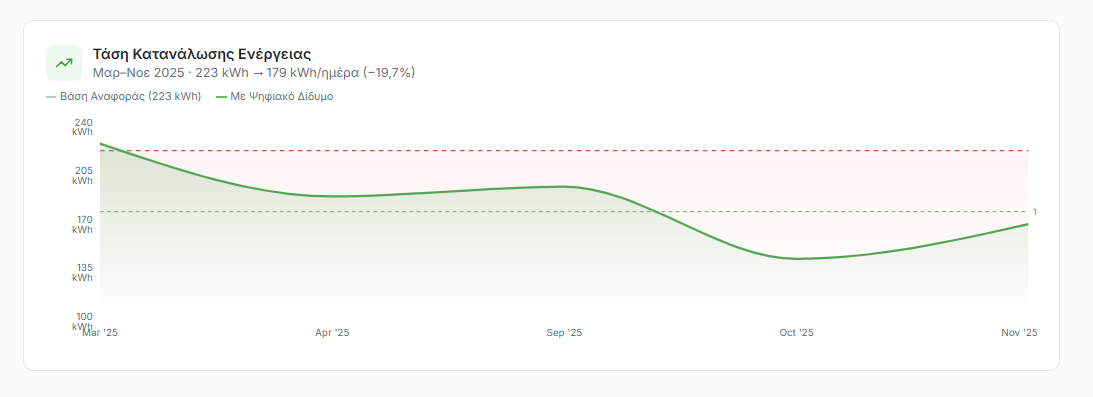
\includegraphics[width=\textwidth]{fig_6_2}
\caption{Διάγραμμα απόσβεσης της επένδυσης και προβολή ταμειακών ροών πενταετίας}
\label{fig:roi_chart}
\end{figure}

Πέραν των οικονομικών δεικτών, η αξιολόγηση της πλατφόρμας περιλαμβάνει και τεχνικούς δείκτες αξιοπιστίας. Κατά την περίοδο Μαρτίου–Νοεμβρίου 2025, το σύστημα παρουσίασε \textlatin{uptime} 99.95\%, τιμή που επιβεβαιώνει την καταλληλότητά του για επιχειρησιακή χρήση 24/7 σε εκπαιδευτικά περιβάλλοντα. Ο μέσος χρόνος διάδοσης δεδομένων από τον αισθητήρα ως την τελική διεπαφή χρήστη (\textlatin{end-to-end latency}) παρέμεινε κάτω από 5 δευτερόλεπτα, επιβεβαιώνοντας τον πραγματικού χρόνου χαρακτήρα της πλατφόρμας.

\begin{table}[htbp]
\centering
\caption{Ενδεικτικός επιμερισμός του συνολικού κόστους επένδυσης (\textlatin{CAPEX})}
\label{tab:capex_breakdown}
\begin{tabular}{|p{4.5cm}|p{6.5cm}|r|}
\hline
\textbf{Κατηγορία} & \textbf{Περιγραφή} & \textbf{Κόστος} \\
\hline
Κόστος Αισθητήρων / \textlatin{Hardware} & \textlatin{Edge \& IoT Nodes (ESP32, Shelly 1PM, Sonoff, ESP8266, DS18B20,} μαγνητικές επαφές, \textlatin{Raspberry Pi 4)} & 245,17~\euro \\
\hline
Κόστος Πλατφόρμας \& \textlatin{Cloud Integration} & \textlatin{Software stack, Supabase, openHAB} παραμετροποίηση, \textlatin{React 18 frontend} ανάπτυξη & 7.500,00 \euro \\
\hline
Κόστος Εγκατάστασης & \textlatin{Deployment}, καλωδιώσεις, δικτύωση, \textlatin{commissioning} στο πεδίο & 7.500,00 \euro \\
\hline
Κόστος Εκπαίδευσης / Παραμετροποίησης & \textlatin{Onboarding}, τεκμηρίωση, τεχνική υποστήριξη πιλοτικής λειτουργίας & 4.306,83 \euro \\
\hline
\textbf{Συνολική Επένδυση (\textlatin{CAPEX})} & & \textbf{19.500,00 \euro} \\
\hline
\end{tabular}
\end{table}

\begin{table}[htbp]
\centering
\caption{Τεχνικοί δείκτες αξιοπιστίας και απόδοσης της πλατφόρμας}
\label{tab:technical_kpis}
\begin{tabular}{|l|l|l|}
\hline
\textbf{Δείκτης} & \textbf{Τιμή} & \textbf{Μέθοδος Επαλήθευσης} \\
\hline
Ακρίβεια Θορύβου (\textlatin{INMP441}) & ±2 \textlatin{dBA} & Σύγκριση με βιομηχανικό ηχόμετρο αναφοράς \\
\hline
Ακρίβεια Θερμοκρασίας (\textlatin{DHT22}) & ±0.5°C & Σύγκριση με βαθμονομημένο θερμόμετρο \\
\hline
Ακρίβεια Υγρασίας (\textlatin{DHT22}) & ±2\% \textlatin{RH} & Σύγκριση με βαθμονομημένο υγρόμετρο \\
\hline
Συνολική Αξιοπιστία Δεδομένων & 98.5\% & Διασταύρωση με όργανα αναφοράς \\
\hline
\textlatin{System Uptime} & 99.95\% & Συνεχής καταγραφή Μαρ–Νοε 2025 \\
\hline
\textlatin{End-to-End Latency} & < 5 \textlatin{sec} & Μέτρηση αισθητήρας $\rightarrow$ \textlatin{UI} \\
\hline
\textlatin{Sensor} $\rightarrow$ \textlatin{MQTT} & $\sim$45 \textlatin{ms} & \textlatin{Network timing analysis} \\
\hline
\textlatin{MQTT} $\rightarrow$ \textlatin{openHAB} & $\sim$28 \textlatin{ms} & \textlatin{openHAB log analysis} \\
\hline
\textlatin{openHAB} $\rightarrow$ \textlatin{UI Update} & $\sim$19 \textlatin{ms} & \textlatin{Browser DevTools} \\
\hline
\end{tabular}
\end{table}

\noindent\textit{Σημείωση: Η κατανομή ανά κατηγορία είναι ενδεικτική. Το συνολικό \textlatin{CAPEX} των 19.500~\euro\ αποτελεί το μέγεθος αναφοράς της τεχνοοικονομικής ανάλυσης.}

\begin{table}[htbp]
\centering
\caption{Εξέλιξη ετήσιων λειτουργικών οφελών και συνοπτικοί δείκτες απόδοσης επένδυσης}
\label{tab:roi_projection}
\begin{tabular}{|l|l|r|}
\hline
\textbf{Περίοδος / Δείκτης} & \textbf{Περιγραφή} & \textbf{Τιμή} \\
\hline
\textlatin{Year 1} & Ετήσια λειτουργικά οφέλη (\textlatin{OPEX Savings}) & 5.500,00 \euro \\
\hline
\textlatin{Year 2} & Σωρευτικά λειτουργικά οφέλη & 11.000,00 \euro \\
\hline
\textlatin{Year 3} & Σωρευτικά λειτουργικά οφέλη & 16.500,00 \euro \\
\hline
\textlatin{Year 5} & Σωρευτικά λειτουργικά οφέλη & 27.500,00 \euro \\
\hline
5-ετές Καθαρό Κέρδος & Μετά την αφαίρεση της αρχικής επένδυσης & 8.000,00 \euro \\
\hline
Περίοδος Απόσβεσης & \textlatin{Payback Period} & 42,5 μήνες \\
\hline
Απόδοση Επένδυσης 5ετίας & \textlatin{5-year ROI} & 41,02\% \\
\hline
\end{tabular}
\end{table}





\chapter{Συζήτηση και Κριτική Αξιολόγηση}

\section{Εισαγωγή στη Συζήτηση των Ευρημάτων}
Η παρούσα διπλωματική εργασία σχεδιάστηκε με γνώμονα τη διερεύνηση της πρακτικής εφαρμοσιμότητας και της προστιθέμενης αξίας των τεχνολογιών Ψηφιακού Διδύμου (\textlatin{Digital Twin}) σε σχολικές υποδομές. Μέσω της πιλοτικής εφαρμογής στα Εκπαιδευτήρια Πλάτων, η έρευνα επιχείρησε να μεταβεί από τη θεωρητική σύλληψη των Έξυπνων Πανεπιστημιουπόλεων (\textlatin{Smart Campuses}) σε μια απτή, μετρήσιμη και τεχνοοικονομικά αξιολογήσιμη εγκατάσταση. Τα αποτελέσματα που παρουσιάστηκαν στο προηγούμενο κεφάλαιο υποστηρίζουν την κεντρική ερευνητική υπόθεση: η ενοποίηση υλικού χαμηλού κόστους (\textlatin{Edge IoT}) με λογισμικό ανοιχτού κώδικα (\textlatin{openHAB, InfluxDB}) δύναται να δημιουργήσει έναν κλειστό βρόχο ελέγχου ο οποίος βελτιώνει ταυτόχρονα το μαθησιακό περιβάλλον και την ενεργειακή αποδοτικότητα. Στο παρόν κεφάλαιο επιχειρείται η εις βάθος ερμηνεία αυτών των ευρημάτων, η σύγκρισή τους με την υφιστάμενη βιβλιογραφία, καθώς και η ανάλυση των περιορισμών και των προκλήσεων που αναδείχθηκαν κατά την επιχειρησιακή λειτουργία του συστήματος.

\section{Ερμηνεία των Αποτελεσμάτων Ποιότητας Εσωτερικού Περιβάλλοντος (\textlatin{IEQ}) και Ακουστικής Άνεσης}
Η Ποιότητα Εσωτερικού Περιβάλλοντος (\textlatin{Indoor Environmental Quality - IEQ}) αποτελεί ίσως τον κρισιμότερο παράγοντα για την εξασφάλιση της υγείας, της γνωστικής απόδοσης και της ψυχολογικής ευεξίας των μαθητών και των εκπαιδευτικών. Ιδιαίτερα η ακουστική άνεση, η οποία συχνά παραβλέπεται κατά τον σχεδιασμό σχολικών κτιρίων σε σχέση με τη θερμική ή την οπτική άνεση, τέθηκε στο επίκεντρο της λειτουργίας του Ψηφιακού Διδύμου.

\subsection{Η Ψυχολογική Προσέγγιση: Παθητική Αυτορρύθμιση Συμπεριφοράς}
Σύμφωνα με τις οδηγίες του Παγκόσμιου Οργανισμού Υγείας (\textlatin{WHO}), τα επίπεδα θορύβου βάθους (\textlatin{background noise}) σε μια άδεια σχολική αίθουσα δεν πρέπει να υπερβαίνουν τα 35 \textlatin{dBA}, ώστε να εξασφαλίζεται επαρκής λόγος σήματος προς θόρυβο (\textlatin{Signal-to-Noise Ratio, SNR $\geq +15$ dB}) για την καθαρότητα της ομιλίας \cite{WHO1999}, \cite{Kephalopoulos2015}. Κατά τη διάρκεια της εκπαιδευτικής διαδικασίας, ωστόσο, τα επίπεδα αυτά ποικίλλουν έντονα. Η αρχική περίοδος αναφοράς (\textlatin{baseline}), όπου το σύστημα λειτουργούσε αμιγώς ως παθητικός καταγραφέας (\textlatin{Digital Shadow}), ανέδειξε συχνές υπερβάσεις του δυναμικού κατωφλίου των 55 \textlatin{dBA}.

Η καινοτομία της παρέμβασης δεν εντοπίζεται απλώς στην καταγραφή, αλλά στη φύση της ανατροφοδότησης (\textlatin{actuation}). Η επιλογή να αποφευχθεί η χρήση ηχητικών συναγερμών (\textlatin{buzzers}) εντός της τάξης υπήρξε απολύτως συνειδητή και επιστημονικά τεκμηριωμένη. Η χρήση ενός επιπρόσθετου ηχητικού ερεθίσματος σε ένα ήδη θορυβώδες περιβάλλον θα προκαλούσε περαιτέρω διάσπαση προσοχής, γνωστική υπερφόρτωση και αυξημένο στρες τόσο στους μαθητές όσο και στον εκπαιδευτικό, διακόπτοντας βίαια τη ροή του μαθήματος.

Αντιθέτως, η ενεργοποίηση μιας διακριτικής οπτικής ένδειξης (\textlatin{quiet-lamp}) λειτούργησε ως ένας μηχανισμός "παθητικής αυτορρύθμισης" (\textlatin{passive behavioral nudging}). Όταν το σύστημα αντιλαμβανόταν συνεχή υπέρβαση του ορίου των 55 \textlatin{dBA} για ένα προκαθορισμένο χρονικό διάστημα (π.χ. 20 δευτερόλεπτα), άναβε τη λυχνία. Η οπτική αυτή ειδοποίηση επέτρεψε στους μαθητές να αντιληφθούν μόνοι τους την αύξηση της έντασης και να χαμηλώσουν τον τόνο της φωνής τους, ενώ ταυτόχρονα παρείχε στον εκπαιδευτικό ένα αντικειμενικό εργαλείο διαχείρισης της τάξης. Η σημαντική μείωση στον αριθμό και τη διάρκεια των υπερβάσεων του ορίου που αποτυπώνεται στο Σχήμα~\ref{fig:noise_results} κατά τη δεύτερη φάση λειτουργίας, υποστηρίζει ότι οι τεχνολογίες \textlatin{IoT} δεν χρησιμεύουν μόνο για τη μηχανολογική διαχείριση ενός κτιρίου, αλλά μπορούν να διαδραματίσουν ενεργό παιδαγωγικό ρόλο, βελτιώνοντας την ακουστική άνεση και μειώνοντας την κόπωση (\textlatin{vocal fatigue}) των διδασκόντων.

\section{Ενεργειακή Βελτιστοποίηση και Τεχνοοικονομική Σκοπιμότητα στη Διαχείριση Εγκαταστάσεων (\textlatin{Facility Management})}
Στον άξονα της ενεργειακής αποδοτικότητας, το Ψηφιακό Δίδυμο μετατράπηκε από ένα εργαλείο ευεξίας σε ένα αυστηρό σύστημα Διαχείρισης Εγκαταστάσεων (\textlatin{Facility Management}) και Προγνωστικής Συντήρησης (\textlatin{Predictive Maintenance}). Η μείωση της μέσης ημερήσιας κατανάλωσης κατά 19,7\% (από 223 σε 179 \textlatin{kWh}/ημέρα) αποτελεί ένα πρακτικά σημαντικό και εμπορικά κρίσιμο εύρημα.

\subsection{Η Αντιμετώπιση των Κρυφών Φορτίων (\textlatin{Phantom Loads})}
Τα σχολικά συγκροτήματα παρουσιάζουν εξαιρετικά ασυνεχή προφίλ κατανάλωσης. Παρατηρούνται ακραίες αιχμές ζήτησης κατά τις πρωινές ώρες λειτουργίας και σχεδόν μηδενική ζήτηση τα απογεύματα, τα Σαββατοκύριακα και τις περιόδους διακοπών. Παρά ταύτα, η ανάλυση των δεδομένων της περιόδου αναφοράς (πριν την εφαρμογή του συστήματος) ανέδειξε σημαντική κατανάλωση ενέργειας κατά τις ώρες αδράνειας. Αυτό οφείλεται κυρίως στα «κρυφά» φορτία (\textlatin{phantom loads}), δηλαδή σε συσκευές που παραμένουν σε λειτουργία ή σε κατάσταση αναμονής χωρίς ουσιαστικό λόγο.

Χαρακτηριστικό παράδειγμα αποτέλεσε ο εξοπλισμός του κυλικείου. Μέσω της τοποθέτησης των έξυπνων μετρητών \textlatin{Shelly 1PM} και των αισθητήρων κατάστασης θύρας (\textlatin{reed switches}), το σύστημα άρχισε να καταγράφει τη συχνότητα ανοίγματος των θυρών των επαγγελματικών ψυγείων και την αντίστοιχη άσκοπη λειτουργία του συμπιεστή. Η εγκαθίδρυση του κανόνα \textlatin{FridgeGuardian} στο \textlatin{openHAB} (ενεργοποίηση τοπικού βομβητή όταν η πόρτα παρέμενε ανοιχτή πέραν ενός χρονικού ορίου) περιόρισε αισθητά τις απώλειες ψύξης. Ιδιαίτερα σημαντική ήταν η \textlatin{Year-over-Year} (\textlatin{YoY}) σύγκριση του Νοεμβρίου, όπου καταγράφηκε μείωση της τάξης του 32,5\% (από 252 \textlatin{kWh}/ημέρα τον Νοέμβριο του 2024 σε 170 \textlatin{kWh}/ημέρα τον Νοέμβριο του 2025). Αντιθέτως, οι μήνες Σεπτέμβριος και Οκτώβριος 2025 εμφανίζουν οριακή αύξηση μετρούμενης κατανάλωσης σε σχέση με το 2024 (βλ. Παράρτημα Β, Πίνακας Β.2), γεγονός που αποδίδεται στη διεύρυνση του αισθητηριακού δικτύου και στην παράλληλη λειτουργία του τοπικού \textlatin{MVP} και της \textlatin{cloud} πλατφόρμας κατά τη μεταβατική περίοδο ωρίμανσης του συστήματος. Η αιχμή αυτή της εξοικονόμησης υποστηρίζει την αποτελεσματικότητα του αμφίδρομου ελέγχου (κλείσιμο διακοπτών, απενεργοποίηση φορτίων εκτός ωραρίου) κατά τους πλέον ενεργοβόρους χειμερινούς μήνες.

Η ερμηνεία της έντονης μείωσης του Νοεμβρίου απαιτεί διαχωρισμό των συνιστωσών φορτίου. Με βάση την ανάλυση γεγονότων της πλατφόρμας, το ισχυρότερο αποτύπωμα εντοπίζεται στον περιορισμό των \textlatin{phantom loads} και στη βελτίωση της λειτουργίας του ψυκτικού εξοπλισμού του κυλικείου (χρόνος ανοιχτής πόρτας, κύκλοι συμπιεστή). Η συμβολή φορτίων θέρμανσης/κλιματισμού (\textlatin{HVAC}) δεν μπορεί να ποσοτικοποιηθεί πλήρως στο παρόν \textlatin{dataset}, καθώς δεν υπάρχει ανεξάρτητη υπομέτρηση ανά υποσύστημα. Παρόλα αυτά, η συνέπεια των καταγραφών \textlatin{FridgeGuardian} και των χρονοσειρών ισχύος υποστηρίζει ότι η κύρια συνεισφορά του 32,5\% προέρχεται από τη μείωση λειτουργικών απωλειών και όχι από μεμονωμένη εποχική διακύμανση.

\subsection{Ανάλυση Κόστους Κύκλου Ζωής (\textlatin{LCC}) και \textlatin{ROI}}
Η τεχνοοικονομική μελέτη (\textlatin{ROI Calculator}) κατέδειξε περίοδο απόσβεσης (\textlatin{Payback Period}) 42,5 μηνών και 5ετές \textlatin{ROI} της τάξης του 41,02\%\footnote{Σημείωση: Η οπτικοποίηση της πλατφόρμας (Σχήμα~5.1) εμφανίζει τιμή 41{,}44\% λόγω ελαφρά διαφορετικής στρογγυλοποίησης της παραμέτρου ετήσιας εξοικονόμησης. Η τιμή αναφοράς της παρούσας ανάλυσης είναι 41{,}02\%.}. Τα νούμερα αυτά αποκτούν ακόμη μεγαλύτερη βαρύτητα εάν συγκριθούν με τα παραδοσιακά Συστήματα Διαχείρισης Κτιρίων (\textlatin{Building Management Systems - BMS}). Ένα τυπικό \textlatin{BMS} κλειστής αρχιτεκτονικής συνεπάγεται αυξημένο αρχικό κόστος κεφαλαίου (\textlatin{CAPEX}) για καλωδιώσεις, ιδιόκτητα πρωτόκολλα (\textlatin{proprietary hardware}) και υψηλότερα κόστη συντήρησης (\textlatin{OPEX}) με ετήσιες άδειες χρήσης λογισμικού.

Αντιθέτως, το προτεινόμενο σύστημα βασίστηκε στην προσέγγιση του "\textlatin{Brownfield Integration}", δηλαδή στην ενσωμάτωση του υφιστάμενου εξοπλισμού σε ένα σύγχρονο \textlatin{IoT} δίκτυο, χωρίς να απαιτείται ξήλωμα ή συνολική αντικατάσταση των υφιστάμενων υποδομών. Η προσέγγιση αυτή μειώνει το κόστος μετάβασης, ενισχύει τη διαλειτουργικότητα, συνάδει με αντίστοιχες ευρωπαϊκές μελέτες για ενεργειακή βελτιστοποίηση κτιρίων \cite{Apostolopoulos2022}, \cite{Fokaides2020}, και εναρμονίζεται πλήρως με τις απαιτήσεις της αναθεωρημένης Ευρωπαϊκής Οδηγίας για την Ενεργειακή Απόδοση Κτιρίων \cite{EUParliament2024}.

Ιδιαίτερη σημασία έχει και η εξελικτική μετάβαση από το αρχικό \textlatin{MVP}, το οποίο εξυπηρετούσε κυρίως την τοπική συλλογή δεδομένων και την επιβεβαίωση των κανόνων ελέγχου, προς την τελική \textlatin{Cloud} πλατφόρμα ανάλυσης. Η μεταφορά των δεικτών κόστους, των αναφορών \textlatin{ROI} και των προβολών εξοικονόμησης σε ένα περισσότερο φιλικό, διαδικτυακά προσβάσιμο περιβάλλον βελτίωσε ουσιαστικά τη χρηστικότητα του συστήματος για μη τεχνικούς ρόλους, όπως ο διευθυντής της σχολικής μονάδας, ο οποίος μπορούσε πλέον να παρακολουθεί συγκεντρωτικά την απόδοση της επένδυσης χωρίς να εξαρτάται από τεχνικά εργαλεία τοπικής διαχείρισης.

\section{Θεωρητική Ανάλυση: Η Μετάβαση από την Ψηφιακή Σκιά στο Ψηφιακό Δίδυμο}
Στον ακαδημαϊκό χώρο της Πληροφορικής και της Μηχανικής, παρατηρείται συχνά μια εσφαλμένη ταύτιση της απλής τηλεμετρίας \textlatin{IoT} ή των τρισδιάστατων σχεδίων \textlatin{BIM} με τον όρο "Ψηφιακό Δίδυμο". Σύμφωνα με την ταξινόμηση που διατυπώθηκε αρχικά στο βιομηχανικό πλαίσιο \cite{Kritzinger2018} και εφαρμόζεται ευρέως στον κτιριακό τομέα \cite{Fuller2020}, \cite{Grieves2017}, απαιτείται σαφής διαχωρισμός τριών βαθμίδων:
\begin{itemize}
\item \textbf{\textlatin{Digital Model}:} Η στατική ψηφιακή αναπαράσταση χωρίς αυτόματη ροή δεδομένων (π.χ. ένα σχέδιο \textlatin{CAD}).
\item \textbf{\textlatin{Digital Shadow}:} Η ψηφιακή αναπαράσταση που λαμβάνει αυτόματα δεδομένα από το φυσικό αντικείμενο (μονόδρομη ροή - \textlatin{Sense}), όπως τα περισσότερα \textlatin{IoT Dashboards}.
\item \textbf{\textlatin{Digital Twin}:} Το σύστημα όπου υφίσταται αμφίδρομη ροή (\textlatin{bidirectional data flow}). Τα δεδομένα του φυσικού χώρου ενημερώνουν τον ψηφιακό, και οι αλγοριθμικές αποφάσεις του ψηφιακού χώρου επιφέρουν άμεση φυσική μεταβολή (\textlatin{Actuation}).
\end{itemize}

Η παρούσα εργασία γεφυρώνει αυτό το ακαδημαϊκό κενό, τεκμηριώνοντας πρακτικά την εφαρμογή της τρίτης και ανώτατης βαθμίδας. Μέσω της αρχιτεκτονικής του \textlatin{openHAB}, το οποίο λειτούργησε ως σημασιολογικό ενδιάμεσο λογισμικό (\textlatin{semantic middleware}), υλοποιήθηκε ο πλήρης κύκλος \textit{\textlatin{Sense-Decide-Act}}. Ο μικροελεγκτής \textlatin{ESP32} ανιχνεύει τον θόρυβο (\textlatin{Sense}), αποστέλλει τα δεδομένα μέσω \textlatin{MQTT} στον κεντρικό διακομιστή \textlatin{Raspberry Pi}, η μηχανή κανόνων (\textlatin{Rules Engine}) αποφασίζει βάσει του ορίου των 55 \textlatin{dBA} και του σχολικού ωραρίου (\textlatin{Decide}), και τέλος, το σύστημα αποστέλλει εντολή ελέγχου στο ρελέ \textlatin{Sonoff} για να ανάψει η φυσική λάμπα εντός της τάξης (\textlatin{Act}). Η διπλή αυτή κατεύθυνση των δεδομένων υποστηρίζει τον χαρακτηρισμό της πλατφόρμας ως ένα πραγματικό Ψηφιακό Δίδυμο, διαχωρίζοντάς την από τα συμβατικά συστήματα τηλεμετρίας (\textlatin{Digital Shadows}).

\section{Προκλήσεις, Περιορισμοί και Επεκτασιμότητα (\textlatin{Scalability})}
Η εξαγωγή συμπερασμάτων από μια μελέτη περίπτωσης (\textlatin{case study}) σε πραγματικό περιβάλλον οφείλει να συνοδεύεται από κριτική εξέταση των περιορισμών της εφαρμογής και των προκλήσεων που ενδέχεται να προκύψουν κατά την κλιμάκωση (\textlatin{scalability}) του συστήματος σε άλλα σχολικά συγκροτήματα.

\subsection{Τεχνικοί Περιορισμοί και Εξάρτηση Δικτύου}
Ο πρώτος σημαντικός περιορισμός αφορά την αξιοπιστία της δικτυακής υποδομής. Εφόσον το σύνολο των κόμβων \textlatin{IoT} (\textlatin{Edge Nodes}) χρησιμοποιεί το ασύρματο τοπικό δίκτυο (\textlatin{Wi-Fi}) του σχολείου για την επικοινωνία με τον \textlatin{MQTT Broker}, τυχόν αστάθεια ή διακοπή λειτουργίας των \textlatin{Access Points} (\textlatin{AP}) οδηγεί σε προσωρινή απώλεια τηλεμετρίας. Για την αντιμετώπιση αυτού του κινδύνου σε μελλοντικές εγκαταστάσεις μεγάλων διαστάσεων (\textlatin{multi-building campuses}), προτείνεται η χρήση πρωτοκόλλων χαμηλής ισχύος και μεγάλης εμβέλειας, όπως το \textlatin{LoRaWAN} ή η δημιουργία απομονωμένων δικτύων \textlatin{Zigbee/Matter}, τα οποία δεν εξαρτώνται από το εμπορικό δίκτυο \textlatin{Wi-Fi} του ιδρύματος.

\subsection{Τοπική Επεξεργασία στην Παρυφή και Αποδοτικότητα Δικτύου}
Μια από τις σημαντικότερες τεχνικές προκλήσεις κατά την εισαγωγή αισθητήρων (ειδικά μικροφώνων) σε σχολικές αίθουσες είναι η διατήρηση χαμηλού δικτυακού φόρτου και η σταθερότητα του συστήματος σε πραγματικές συνθήκες λειτουργίας. Για τον λόγο αυτό, η αρχιτεκτονική του συστήματος σχεδιάστηκε με έμφαση στην τοπική επεξεργασία (\textlatin{edge processing}) αντί της αποστολής ακατέργαστων ροών στο \textlatin{cloud}. Η επιλογή αυτή μειώνει σημαντικά το απαιτούμενο εύρος ζώνης και αποτρέπει την υπερφόρτωση του δικτύου σε ώρες αιχμής.

Ο μικροελεγκτής \textlatin{ESP32} συλλέγει το ηχητικό σήμα μέσω του πρωτοκόλλου \textlatin{I2S} και υπολογίζει τοπικά τη Μέση Στάθμη Ηχητικής Πίεσης (\textlatin{Equivalent Continuous Sound Level - LAeq}) σε \textlatin{decibel} (\textlatin{dBA}) εντός πτητικής μνήμης (\textlatin{RAM}). Προς τον κεντρικό διακομιστή αποστέλλεται αποκλειστικά η συμπυκνωμένη αριθμητική τιμή (π.χ. 58.2 \textlatin{dBA}), γεγονός που περιορίζει τον όγκο τηλεμετρίας ανά κόμβο. Σε συνδυασμό με την ασφάλεια δικτύου (κρυπτογραφημένες ζεύξεις, έλεγχος πρόσβασης και απομόνωση υπηρεσιών), το σύστημα επιτυγχάνει ανθεκτική και αποδοτική λειτουργία σε επίπεδο \textlatin{campus}.

\subsection{Γενικευσιμότητα (\textlatin{Generalizability}) και Κουλτούρα Χρηστών}
Προκειμένου ένα τέτοιο σύστημα να επεκταθεί σε περιφερειακό επίπεδο (π.χ. σε όλα τα δημόσια σχολεία ενός Δήμου), πρέπει να υπερκεραστεί το εμπόδιο της εξοικείωσης των χρηστών. Το διδακτικό προσωπικό και η διοίκηση του σχολείου πρέπει να εκπαιδευτούν ώστε να αντιμετωπίζουν την πλατφόρμα όχι ως "εργαλείο παρακολούθησης της εργασίας τους", αλλά ως βοηθό για τη βελτίωση του μαθησιακού περιβάλλοντος. Η σχεδίαση της διεπαφής (\textlatin{3D Dashboard} σε \textlatin{React}) έλαβε υπόψη αυτή την ανάγκη, παρέχοντας ένα ιδιαίτερα φιλικό περιβάλλον χρήστη (\textlatin{UX}) που δεν απαιτεί γνώσεις προγραμματισμού ή μηχανικού αυτοματισμών, καθιστώντας την τεχνολογία προσιτή στον τελικό χρήστη.

\subsection{Τεχνικές Προκλήσεις και Μαθήματα από την Υλοποίηση}
Η πιλοτική εφαρμογή σε πραγματικό σχολικό περιβάλλον ανέδειξε πέντε κρίσιμα τεχνικά ζητήματα, η αντιμετώπιση των οποίων εμπλούτισε σημαντικά το αρχιτεκτονικό αποτύπωμα της πλατφόρμας.

Πρώτον, η αρχιτεκτονική συγχρονισμού δεδομένων προκαλούσε καθυστέρηση άνω των 500ms στην ενημέρωση του \textlatin{frontend}, με αποτέλεσμα μη αποδεκτή εμπειρία χρήστη για πραγματικού χρόνου εποπτεία. Η λύση υλοποιήθηκε μέσω \textlatin{WebSocket} συνδέσεων (\textlatin{Supabase Realtime}) με \textlatin{optimistic updates} και \textlatin{connection pooling}, μειώνοντας την καθυστέρηση σε επίπεδα κάτω των 100ms. Το κύριο δίδαγμα είναι ότι η υποδομή πραγματικού χρόνου πρέπει να σχεδιάζεται εξαρχής και όχι να προστίθεται εκ των υστέρων.

Δεύτερον, τα αρχικά τρισδιάστατα μοντέλα προκαλούσαν πτώση του ρυθμού καρέ (\textlatin{frame rate}) κάτω των 30fps σε μεσαίας κατηγορίας συσκευές, υποβαθμίζοντας την εμπειρία χρήστη. Η λύση περιελάμβανε υλοποίηση \textlatin{Level of Detail (LOD)}, \textlatin{lazy loading} τρισδιάστατων στοιχείων και βελτιστοποιήσεις \textlatin{React Three Fiber} (\textlatin{instanced meshes, object pooling}).

Τρίτον, η ετερογένεια πρωτοκόλλων (\textlatin{MQTT} για \textlatin{ESP32}, \textlatin{HTTP REST} για \textlatin{Shelly 1PM}, \textlatin{GPIO} για αισθητήρες επαφής) δημιουργούσε πολυπλοκότητα ολοκλήρωσης. Η υιοθέτηση του \textlatin{openHAB} ως ενιαίου \textlatin{semantic middleware} επέλυσε το ζήτημα, παρέχοντας κοινό \textlatin{REST API} για όλες τις συσκευές ανεξαρτήτως πρωτοκόλλου.

Τέταρτον, οι αισθητήρες θερμοκρασίας και υγρασίας εμφάνισαν σταδιακή απόκλιση (\textlatin{drift}) με την πάροδο του χρόνου, υποβαθμίζοντας αθόρυβα την ακρίβεια των δεδομένων. Η λύση περιελάμβανε αυτοματοποιημένες ρουτίνες βαθμονόμησης και αγωγούς επαλήθευσης δεδομένων (\textlatin{data validation pipelines}) με ανίχνευση εκτός-ορίων τιμών.

Πέμπτον, ο σχεδιασμός απομόνωσης δεδομένων ανά οργανισμό (\textlatin{multi-tenancy}) σε συνδυασμό με αποδεκτή απόδοση ερωτημάτων αποτέλεσε αρχιτεκτονική πρόκληση. Η αξιοποίηση των \textlatin{Row-Level Security (RLS)} πολιτικών της \textlatin{Supabase/PostgreSQL} με \textlatin{SECURITY DEFINER} βοηθητικές συναρτήσεις επέτρεψε την εφαρμογή ασφάλειας σε επίπεδο βάσης δεδομένων, απλοποιώντας σημαντικά τον κώδικα εφαρμογής.

Συνολικά, τα ανωτέρω τεχνικά μαθήματα επιβεβαιώνουν ότι η ανάπτυξη ενός πραγματικού Ψηφιακού Διδύμου σε εκπαιδευτικό περιβάλλον απαιτεί όχι μόνο θεωρητική γνώση αλλά και επαναληπτική μηχανική (\textlatin{iterative engineering}) σε συνθήκες πεδίου.

\subsection{Ηθικές Παράμετροι Εγκατάστασης}
Η εγκατάσταση αισθητηριακού δικτύου σε ενεργό εκπαιδευτικό χώρο με ανήλικους μαθητές εγείρει ζητήματα που απαιτούν ρητή αντιμετώπιση. Καταρχάς, το σύστημα δεν καταγράφει ηχητικό περιεχόμενο (φωνές, συνομιλίες): οι κόμβοι \textlatin{ESP32} υπολογίζουν αποκλειστικά τη στάθμη ηχητικής πίεσης (\textlatin{LAeq} σε \textlatin{dBA}) εντός πτητικής μνήμης και αποστέλλουν μόνο την αριθμητική τιμή στον \textlatin{broker}. Δεύτερον, η εγκατάσταση πραγματοποιήθηκε με πλήρη γνώση και έγγραφη συναίνεση της διοίκησης των Εκπαιδευτηρίων Πλάτων, η οποία ενημερώθηκε για τον σκοπό, τη φύση και τα όρια της συλλογής δεδομένων. Τρίτον, κανένα δεδομένο ταυτοποίησης προσώπου (όνομα, εικόνα, φωνή) δεν συλλέγεται ή αποθηκεύεται από το σύστημα, διασφαλίζοντας την πλήρη ανωνυμία των μαθητών και του εκπαιδευτικού προσωπικού.

\section{Ευθυγράμμιση με Ευρωπαϊκές Πολιτικές και το Όραμα των \textlatin{Smart Campuses}}
Τα ευρήματα της παρούσας μελέτης βρίσκονται σε ισχυρή εναρμόνιση με το μακροπρόθεσμο στρατηγικό πλαίσιο της Ευρωπαϊκής Ένωσης. Το πρόγραμμα \textit{\textlatin{DIGITAL EUROPE}} δίνει ρητή έμφαση στη δημιουργία Τοπικών Ψηφιακών Διδύμων (\textlatin{Local Digital Twins}) για αστικές και κοινοτικές υποδομές \cite{EuropeanCommission2023}. Η εφαρμογή αυτής της στρατηγικής σε εκπαιδευτικά κτίρια αποτελεί φυσική επέκταση του ευρωπαϊκού οράματος ψηφιακού μετασχηματισμού, ευθυγραμμιζόμενη παράλληλα με τις ενεργειακές απαιτήσεις της αναθεωρημένης Οδηγίας για την Ενεργειακή Απόδοση Κτιρίων \cite{EUParliament2024}.

Επιπρόσθετα, η εισαγωγή του Ψηφιακού Διδύμου στην εκπαιδευτική βαθμίδα δημιουργεί μετρήσιμες ευκαιρίες εφαρμογής STEM εντός του σχολικού χώρου. Η σχολική εγκατάσταση παύει να είναι απλώς ένα στατικό κέλυφος και μετατρέπεται σε ένα ``Ζωντανό Εργαστήριο'' (\textlatin{Living Lab}). Οι μαθητές έρχονται σε άμεση επαφή με ζωντανά δεδομένα (Big Data, IoT, περιβαλλοντικοί δείκτες), γεγονός που μπορεί να ενισχύσει τα προγράμματα εκπαίδευσης STEM (Επιστήμη, Τεχνολογία, Μηχανική, Μαθηματικά) και να καλλιεργήσει ενεργά την περιβαλλοντική τους συνείδηση. Η διπλωματική αυτή υποστηρίζει ότι τα Ψηφιακά Δίδυμα δεν αποτελούν προνόμιο αποκλειστικά της βαριάς βιομηχανίας (\textlatin{Industry 4.0}), αλλά μια ώριμη, προσβάσιμη τεχνολογία ικανή να μετασχηματίσει το σύγχρονο εκπαιδευτικό οικοσύστημα (\textlatin{Education 4.0}).

\section{Διαλειτουργικότητα (\textlatin{Interoperability}) και Ενσωμάτωση Υφιστάμενων Υποδομών}
Ένα από τα σημαντικότερα τεχνικά επιτεύγματα της παρούσας μελέτης είναι η απόδειξη της έννοιας της διαλειτουργικότητας (\textlatin{interoperability}) και της πρακτικής εφαρμογής του '\textlatin{Brownfield Integration}'. Στη βιομηχανία, η αναβάθμιση σε ένα ψηφιακό οικοσύστημα σπάνια συνεπάγεται την πλήρη αποξήλωση του παλαιού εξοπλισμού. Η πραγματική πρόκληση για έναν Μηχανικό είναι η ενοποίηση υφιστάμενων (\textlatin{legacy}) υποδομών με τις σύγχρονες τεχνολογίες Διαδικτύου των Πραγμάτων (\textlatin{IoT}).

Το σύστημα που αναπτύχθηκε υπερβαίνει κατά πολύ τον απλό 'Ψηφιακό Σκιασμό' (\textlatin{Digital Shadow}), ο οποίος περιορίζεται στη μονόδρομη ροή δεδομένων για την απλή οπτικοποίηση. Αντιθέτως, μεταβαίνει στο επίπεδο ενός πραγματικού Ψηφιακού Διδύμου (\textlatin{true Digital Twin}) μέσω της εγκαθίδρυσης αμφίδρομης επικοινωνίας και ελέγχου. Χαρακτηριστικότερο παράδειγμα αυτής της μετάβασης αποτελεί η επιτυχής ενσωμάτωση της υφιστάμενης υποδομής \textlatin{PLC (Programmable Logic Controller)} που διέθετε το σχολείο για τον έλεγχο των πυλών οχημάτων (\textlatin{vehicular gates}). Αντί να αντικατασταθούν τα βαρέα μοτέρ και οι ελεγκτές, τοποθετήθηκαν ρελέ ξηρής επαφής (\textlatin{dry-contact relays}) τα οποία επικοινωνούν μέσω πρωτοκόλλου \textlatin{MQTT}.

Η προσέγγιση αυτή επέτρεψε τον απομακρυσμένο έλεγχο των πυλών απευθείας από την τρισδιάστατη διεπαφή (\textlatin{3D Dashboard}) της πλατφόρμας. Σε συνδυασμό με τους \textlatin{MQTT-based} ενεργοποιητές (\textlatin{actuators}) για την ανατροφοδότηση του θορύβου μέσα στις σχολικές αίθουσες (έλεγχος οπτικής λυχνίας), η πλατφόρμα τεκμηριώνει την ικανότητά της να γεφυρώνει συστήματα διαφορετικών κατασκευαστών και γενεών. Η επιτυχία αυτού του εγχειρήματος αποδυναμώνει την αντίληψη ότι τα Έξυπνα Σχολεία (\textlatin{Smart Campuses}) απαιτούν εξαιρετικά υψηλά κόστη υλοποίησης και κλειστές αρχιτεκτονικές \textlatin{BMS}.

\section{Παιδαγωγική Αξία: Το Ψηφιακό Δίδυμο ως Εκπαιδευτικό Εργαλείο}
Ενώ τα περισσότερα Συστήματα Διαχείρισης Κτιρίων (\textlatin{BMS}) εξυπηρετούν αποκλειστικά τους διαχειριστές της εγκατάστασης (\textlatin{Facility Managers}), η εισαγωγή ενός Ψηφιακού Διδύμου σε ένα σχολικό συγκρότημα προσφέρει μια ανεκτίμητη, παράλληλη εκπαιδευτική διάσταση. Το ίδιο το κτίριο λειτουργεί ως «Ζωντανό Εργαστήριο» (εν. γλγ. \textlatin{Living Lab}) \cite{Li2024}, παρέχοντας στους μαθητές άμεση πρόσβαση σε πραγματικά δεδομένα περιβαλλοντικής παρακολούθησης στο πλαίσιο εφαρμογών \textlatin{STEM}.

\subsection{Εικονικά Εργαστήρια (\textlatin{Virtual Labs}) και Αναλυτική Μάθησης}
Οι αισθητήρες που έχουν εγκατασταθεί για τη λειτουργική διαχείριση παράγουν έναν τεράστιο όγκο ανοιχτών δεδομένων (\textlatin{big data}), τα οποία μπορούν να αξιοποιηθούν στη μαθησιακή διαδικασία. Για παράδειγμα, στο μάθημα της Φυσικής ή της Πληροφορικής, οι μαθητές μπορούν να αντλήσουν τις χρονοσειρές από τη βάση \textlatin{InfluxDB} και να μελετήσουν τη μεταβολή της θερμοκρασίας, να αναλύσουν τη διάδοση των ηχητικών κυμάτων (\textlatin{dBA}) μέσα στην τάξη, ή να υπολογίσουν την ηλεκτρική ισχύ (\textlatin{Watts}) που καταναλώνουν τα ψυγεία.

Αυτή η προσέγγιση προάγει την εκπαίδευση βάσει έργου (\textlatin{Project-Based Learning}). Η πλατφόρμα, μέσω των \textlatin{2D} και \textlatin{3D} δυναμικών κατόψεων (\textlatin{Floorplans}), επιτρέπει τη δημιουργία Εικονικών Εργαστηρίων (\textlatin{Virtual Labs}). Οι μαθητές οπτικοποιούν τις αόρατες μεταβλητές του χώρου τους, καλλιεργούν την περιβαλλοντική τους συνείδηση και κατανοούν πρακτικά τις έννοιες της Εξοικονόμησης Ενέργειας, βλέποντας σε πραγματικό χρόνο τις επιπτώσεις των πράξεών τους (π.χ. τι συμβαίνει στην κατανάλωση όταν αφήνουν μια πόρτα ανοιχτή) \cite{Li2024}.

\section{Προοπτικές Τεχνητής Νοημοσύνης (\textlatin{AI}) και Προγνωστικής Συντήρησης}
Με το θεμέλιο της αναπτυχθείσας πλατφόρμας να είναι πλέον λειτουργικό και σταθερό, διανοίγονται σημαντικές προοπτικές για τη μελλοντική της επέκταση. Ο όγκος των τηλεμετρικών δεδομένων που συγκεντρώνεται καθημερινά, καθιστά το σύστημα έτοιμο για την ενσωμάτωση αλγορίθμων Μηχανικής Μάθησης (\textlatin{Machine Learning - ML}) και αυτόνομων πρακτόρων (\textlatin{AI Agents}).

\subsection{Μετάβαση στο \textlatin{Cognitive Digital Twin}}
Η τρέχουσα υλοποίηση βασίζεται σε προκαθορισμένους, στατικούς κανόνες ελέγχου (\textlatin{rules-based logic}) στο ενδιάμεσο λογισμικό (\textlatin{openHAB}), όπως για παράδειγμα το όριο των 55 \textlatin{dBA}. Το επόμενο εξελικτικό βήμα είναι η μετάβαση σε ένα Γνωστικό Ψηφιακό Δίδυμο (\textlatin{Cognitive Digital Twin}) \cite{Semeraro2021}. Σε αυτό το μοντέλο, οι αλγόριθμοι Τεχνητής Νοημοσύνης θα αναλύουν ιστορικά δεδομένα για να εντοπίζουν δυναμικά τις ιδανικές συνθήκες.

Για παράδειγμα, η ανάλυση ανωμαλιών (\textlatin{Anomaly Detection}) θα μπορούσε να εξετάζει την κατανάλωση ισχύος των κινητήρων του ψυγείου σε συνάρτηση με την εσωτερική θερμοκρασία και τον αριθμό ανοιγμάτων της πόρτας. Εάν το σύστημα εντοπίσει ότι ο συμπιεστής λειτουργεί περισσότερο από το κανονικό για να διατηρήσει την ψύξη, μπορεί να σημάνει συναγερμό για επερχόμενη βλάβη (π.χ. απώλεια ψυκτικού υγρού) πολύ πριν το ψυγείο σταματήσει να λειτουργεί. Η Προγνωστική Συντήρηση (\textlatin{Predictive Maintenance}) αυτής της μορφής ελαχιστοποιεί τον χρόνο διακοπής λειτουργίας (\textlatin{downtime}) και μειώνει δραστικά τα κόστη συντήρησης του εξοπλισμού, επιβεβαιώνοντας τον ρόλο του Ψηφιακού Διδύμου ως ένα ιδιαίτερα ισχυρό εργαλείο για την επιχειρηματική διαχείριση σύγχρονων εγκαταστάσεων.

Σε επόμενο στάδιο, η ίδια υποδομή μπορεί να υποστηρίξει υβριδικά μοντέλα πρόβλεψης (\textlatin{time-series forecasting}) για ημερήσια κατανάλωση, ταξινόμηση συμβάντων λειτουργίας και αυτόματη βελτιστοποίηση \textlatin{setpoints} ανά ζώνη κτιρίου. Στο πλαίσιο αυτό, το \textlatin{AI Energy Forecasting} και οι τεχνικές \textlatin{Predictive Analytics} μπορούν να αποτελέσουν το ενδιάμεσο βήμα ανάμεσα στο σημερινό σύστημα υποστήριξης αποφάσεων και στο μελλοντικό \textlatin{Cognitive Digital Twin}. Παράλληλα, η ενσωμάτωση διεπαφών \textlatin{Voice Assistants} μπορεί να καταστήσει τις σύνθετες αναλύσεις περισσότερο άμεσα προσβάσιμες σε διοικητικούς χρήστες, μεταφέροντας τα αποτελέσματα της τεχνητής νοημοσύνης από το επίπεδο των τεχνικών \textlatin{dashboards} στο επίπεδο της καθημερινής λειτουργικής αξιοποίησης.


\chapter{Συμπεράσματα}

Η παρούσα διπλωματική εργασία σχεδίασε, υλοποίησε και αξιολόγησε μια ολοκληρωμένη πλατφόρμα Ψηφιακού Διδύμου για σχολικές υποδομές, με πιλοτική εφαρμογή στα Εκπαιδευτήρια Πλάτων στην Κατερίνη. Το κεντρικό ερώτημα ήταν αν η ενοποίηση υλικού χαμηλού κόστους με λογισμικό ανοιχτού κώδικα μπορεί να δημιουργήσει έναν κλειστό βρόχο ελέγχου ικανό να βελτιώσει ταυτόχρονα το μαθησιακό περιβάλλον και τη λειτουργική διαχείριση ενός σχολικού κτιρίου. Τα ευρήματα παρουσιάζονται με ακαδημαϊκή ειλικρίνεια --- διαχωρίζοντας αυτό που αποδείχθηκε από αυτό που παρατηρήθηκε.

Το κύριο τεχνολογικό εύρημα είναι ότι η μετάβαση από παθητική παρακολούθηση (\textlatin{Digital Shadow}) σε αυθεντικό Ψηφιακό Δίδυμο είναι εφικτή με \textlatin{COTS} εξοπλισμό κόστους 245,17\euro. Η πλατφόρμα υλοποιεί τον πλήρη κύκλο \textlatin{Sense--Decide--Act} και περιλαμβάνει:

\begin{itemize}
\item Ακουστική παρακολούθηση με αυτόματη ενεργοποίηση \textlatin{quiet-lamp} βάσει ορίου 55 \textlatin{dBA}
\item Παρακολούθηση ψυκτικού εξοπλισμού με \textlatin{FridgeGuardian} και αυτόματες ειδοποιήσεις
\item \textlatin{Cloud SaaS} πλατφόρμα με \textlatin{3D visualization}, \textlatin{RBAC} και \textlatin{LLM-based energy forecasting}
\item \textlatin{Demo} περιβάλλον δημόσιας πρόσβασης στο \textlatin{digitaltwin.pi-tech.gr}
\end{itemize}

Πρόσφατες συστηματικές ανασκοπήσεις επιβεβαιώνουν ότι οι \textlatin{DT} εφαρμογές εστιάζουν κυρίως σε αστικές υποδομές και βιομηχανικά περιβάλλοντα [Doulka, 2024], αφήνοντας ανεξερεύνητο τον τομέα των εκπαιδευτικών κτιρίων --- κενό που η παρούσα εργασία καλύπτει.

Τα βασικά ευρήματα της πιλοτικής εφαρμογής συνοψίζονται ως εξής:

\begin{itemize}
\item Ο κλειστός βρόχος ελέγχου λειτουργεί --- αποδείχθηκε αρχιτεκτονικά και επιχειρησιακά
\item Το \textlatin{FridgeGuardian} εντόπισε δύο ανωμαλίες κατανάλωσης (Ιούλιος και Οκτώβριος 2025) και απέστειλε αυτόματη ειδοποίηση --- πρακτικό παράδειγμα Προγνωστικής Συντήρησης
\item Αλλαγή συμπεριφοράς προσωπικού κυλικείου επιβεβαιώθηκε από το ίδιο το προσωπικό και τεκμηριώνεται από τα γραφήματα ανοιγμάτων θύρας
\item Παρατηρήθηκε μείωση 19,7\% στους λογαριασμούς ρεύματος --- στοιχείο που συσχετίζεται με τις παρεμβάσεις του συστήματος χωρίς να αποδεικνύει αιτιακή σχέση, όπως αναλύεται στο Κεφάλαιο 7
\item Επιτυχής υιοθέτηση από μη τεχνικούς χρήστες --- ο διευθυντής του σχολείου ενσωμάτωσε την πλατφόρμα στην καθημερινή του ροή εργασίας χωρίς εξειδικευμένη κατάρτιση
\end{itemize}

Η οικονομική βιωσιμότητα της πλατφόρμας δεν εξαρτάται από την απόδειξη ενεργειακής εξοικονόμησης. Με κόστος υλικών 245,17\euro\ και εκτιμώμενο ετήσιο κόστος συντήρησης $\sim$1.140\euro, η αποφυγή έστω μίας βλάβης ψυκτικού εξοπλισμού ετησίως --- εκτιμώμενο κόστος 500--1.300\euro\ ανά περιστατικό --- καθιστά την επένδυση οικονομικά βιώσιμη. Η κύρια αξία έγκειται στη λειτουργική εποπτεία 24/7 και στην έγκαιρη ανίχνευση αστοχιών --- λειτουργίες που ευθυγραμμίζονται με τους στόχους του \textlatin{DIGITAL EUROPE} για \textlatin{Local Digital Twins} \cite{EuropeanCommission2023} και της Ευρωπαϊκής Πράσινης Συμφωνίας \cite{EUParliament2024}.

Οι κύριοι περιορισμοί --- απουσία υποδιαίρεσης κατανάλωσης ανά υποσύστημα, περιορισμένο αισθητηριακό δίκτυο και εξάρτηση από \textlatin{WiFi} --- αποτελούν οδηγό για μελλοντική έρευνα. Τα επόμενα φυσικά βήματα περιλαμβάνουν:

\begin{itemize}
\item Εγκατάσταση έξυπνων μετρητών ανά υποσύστημα για απόδειξη αιτιακής σχέσης
\item Επέκταση αισθητηριακού δικτύου με αισθητήρες \textlatin{CO2} και πλήρη κάλυψη αιθουσών
\item Ενσωμάτωση \textlatin{BIM} μοντέλων --- ερευνητικά ώριμο πεδίο που έχει αναλυθεί στον ελληνικό ακαδημαϊκό χώρο [Φίλογλου, 2021· Πούλιος, 2023]
\item Εξέλιξη σε \textlatin{Cognitive Digital Twin} με αλγορίθμους ανίχνευσης ανωμαλιών
\end{itemize}

Η πλατφόρμα --- διαθέσιμη στο \textlatin{digitaltwin.pi-tech.gr} --- είναι ήδη έτοιμη να δεχτεί αυτές τις επεκτάσεις, αποτελώντας λειτουργικό σημείο αναφοράς για μελλοντικές υλοποιήσεις \textlatin{Smart Campus} υποδομών.


\begingroup
\selectlanguage{english}
\phantomsection
\addcontentsline{toc}{chapter}{\greekbibliographytitle}
\bibliographystyle{IEEEtran}
\bibliography{IEEEabrv,references}
\endgroup

\appendix
\chapter*{ΠΑΡΑΡΤΗΜΑΤΑ}
\addcontentsline{toc}{chapter}{ΠΑΡΑΡΤΗΜΑΤΑ}
\chapter{Αναλυτικό Κοστολόγιο Εξοπλισμού (\textlatin{Bill of Materials - BOM})}

Στον παρακάτω πίνακα παρατίθεται το αναλυτικό κόστος του υλικού εξοπλισμού (\textlatin{Hardware}) που χρησιμοποιήθηκε για την ανάπτυξη της πλατφόρμας του Ψηφιακού Διδύμου στα Εκπαιδευτήρια Πλάτων, αποδεικνύοντας τη βιωσιμότητα της προσέγγισης χαμηλού κόστους (\textlatin{Edge COTS}).

\begin{table}[htbp]
\centering
\caption{Αναλυτικός πίνακας κοστολόγησης υλικού εξοπλισμού (\textlatin{BOM}).}
\label{tab:appendix_bom}
\begin{tabular}{@{}cp{9.2cm}ccc@{}}
\toprule
\textbf{A/A} & \textbf{Περιγραφή} & \textbf{Τεμάχια} & \textbf{Τιμή/τεμ (\euro)} & \textbf{Σύνολο (\euro)} \\
\midrule
1 & \textlatin{Raspberry Pi 4 Model B (4GB)} & 1 & 73,92 & 73,92 \\
2 & \textlatin{ESP32 DevKit (WROOM)} & 3 & 8,07 & 24,21 \\
3 & \textlatin{INMP441 I\textlatin{2}S Digital Microphone} & 3 & 3,20 & 9,60 \\
4 & \textlatin{ESP8266 NodeMCU} & 1 & 4,50 & 4,50 \\
5 & \textlatin{Shelly 1PM Mini Gen3} & 1 & 17,26 & 17,26 \\
6 & \textlatin{Sonoff Basic R2} & 4 & 9,90 & 39,60 \\
7 & \textlatin{DS18B20 (Waterproof)} & 1 & 7,14 & 7,14 \\
8 & \textlatin{DFPlayer Mini MP3 Module} & 1 & 3,50 & 3,50 \\
9 & Μαγνητική Επαφή Θύρας \textlatin{MC-38} & 1 & 2,50 & 2,50 \\
\midrule
\multicolumn{4}{r}{\textbf{ΣΥΝΟΛΟ}} & \textbf{182,23 \euro} \\
\bottomrule
\end{tabular}
\end{table}

\noindent \textit{Σημείωση 1: Το σύνολο του παρόντος πίνακα (182,23 \euro) αφορά αποκλειστικά τον πιλοτικό \textlatin{edge} εξοπλισμό υλικού (\textlatin{hardware BOM}). Η τεχνοοικονομική ανάλυση παρουσιάζεται στην Ενότητα~5.4 και τα αποτελέσματα στην Ενότητα~6.3.}

\noindent \textit{Σημείωση 2: Οι αισθητήρες \textlatin{INMP441} (Α/Α 3) λειτουργούν σε συνδυασμό με τους \textlatin{ESP32} (Α/Α 2) μέσω πρωτοκόλλου \textlatin{I\textlatin{2}S}.}

\chapter{Δεδομένα Ενεργειακής Κατανάλωσης και Αξιολόγησης}

\noindent Τα δεδομένα του παρόντος παραρτήματος παρουσιάζονται ως περιγραφική στατιστική της περιόδου παρακολούθησης. Η παρατηρηθείσα μείωση κατανάλωσης συσχετίζεται με την εγκατάσταση του συστήματος αλλά δεν αποδεικνύει αιτιακή σχέση λόγω απουσίας υποδιαίρεσης κατανάλωσης ανά υποσύστημα.

Τα παρακάτω δεδομένα προέρχονται από τους επίσημους λογαριασμούς ηλεκτρικής ενέργειας (\texttt{Τριφασική παροχή 135 \textlatin{kVA}}) της εγκατάστασης. Η σύγκριση πραγματοποιείται μεταξύ της περιόδου αναφοράς (ΠΡΙΝ την εγκατάσταση, Σεπ. 2024 -- Φεβ. 2025, Πάροχος: \textlatin{Protergia}) και της περιόδου βελτιστοποίησης (ΜΕΤΑ την εγκατάσταση, Μάι. 2025 -- Νοε. 2025, Πάροχος: \textlatin{NRG}). Ο Πίνακας Β.1 αποτυπώνει τη μη σταθμισμένη σύγκριση σε επίπεδο λογαριασμών, ενώ ο κύριος δείκτης 19,7\% της εργασίας προκύπτει από ξεχωριστή σταθμισμένη κανονικοποίηση μόνο για ημέρες πλήρους σχολικής λειτουργίας.

Η αλλαγή παρόχου μεταξύ των δύο περιόδων (\textlatin{Protergia} $\rightarrow$ \textlatin{NRG}) αποτελεί περιορισμό της σύγκρισης, καθώς ενδέχεται να επηρεάζει τις χρεώσεις δικτύου. Ωστόσο, η τιμή ενέργειας (\euro/\textlatin{kWh}) παρέμεινε σταθερή στα 0,162~\euro/\textlatin{kWh} και στις δύο περιόδους, διασφαλίζοντας συγκρισιμότητα στο επίπεδο κατανάλωσης.

\begin{table}[htbp]
\centering
\caption{Μη σταθμισμένη συγκριτική αποτύπωση βασικών ενεργειακών μετρικών σε επίπεδο λογαριασμών.}
\label{tab:appendix_energy_summary}
\begin{tabular}{@{}p{4.4cm}p{4.2cm}p{4.6cm}p{3.2cm}@{}}
\toprule
\textbf{Μετρική} & \textbf{Περίοδος Αναφοράς (ΠΡΙΝ)} & \textbf{Περίοδος Ψηφιακού Διδύμου (ΜΕΤΑ)} & \textbf{Ποσοστιαία Αλλαγή} \\
\midrule
\textbf{Περίοδος Μέτρησης} & Σεπ. 2024 -- Φεβ. 2025 & Μάι. 2025 -- Νοε. 2025 & -- \\
\textbf{Σύνολο Ημερών} & 122 τιμολογημένες ημέρες & 212 τιμολογημένες/έγκυρες ημέρες & -- \\
\textbf{Μέση Τιμή Ενέργειας} & 0,162 \euro/\textlatin{kWh} & 0,162 \euro/\textlatin{kWh} & 0,0\% \\
\textbf{Μέση Ημερήσια Κατανάλωση} & \textbf{201 \textlatin{kWh}/ημέρα} & \textbf{179 \textlatin{kWh}/ημέρα} & \textbf{-10,9\%*} \\
\bottomrule
\end{tabular}
\end{table}

\noindent Η επίδραση της αποκοπής των ``κρυφών φορτίων'' (\textlatin{phantom loads}) αποτυπώνεται σαφέστερα στη σύγκριση ίδιων μηνών (\textlatin{Year-over-Year}) του Πίνακα Β.2, με την ισχυρότερη βελτίωση να εμφανίζεται στον Νοέμβριο.

\begin{table}[htbp]
\centering
\caption{Αναλυτική μηνιαία σύγκριση κατανάλωσης (\textlatin{YoY} και \textlatin{vs Baseline}).}
\label{tab:appendix_energy_yoy}
\begin{tabular}{@{}lcccc@{}}
\toprule
\textbf{Μήνας} & \textbf{\textlatin{kWh}/ημέρα 2024} & \textbf{\textlatin{kWh}/ημέρα 2025} & \textlatin{YoY} \textbf{Μεταβολή} & \textbf{\textlatin{vs Baseline (223)}} \\
\midrule
Σεπτέμβριος & 163 & 197 & +20,9\% & -11,7\% \\
Οκτώβριος & 134 & 145 & +8,2\% & -35,0\% \\
Νοέμβριος & 252 & 170 & -32,5\% & -23,8\% \\
\bottomrule
\end{tabular}
\end{table}

\noindent Η στήλη ``\textlatin{YoY} Μεταβολή'' συγκρίνει τον ίδιο μήνα μεταξύ 2024 και 2025, αντανακλώντας εποχιακές και λειτουργικές συνθήκες. Η στήλη ``\textlatin{vs Baseline}'' συγκρίνει κάθε μήνα με τη σταθμισμένη μέση ημερήσια κατανάλωση της περιόδου αναφοράς (223 \textlatin{kWh}/ημέρα, Σεπ. 2024 -- Φεβ. 2025). Και οι δύο μετρικές είναι ορθές και απαντούν σε διαφορετικά ερευνητικά ερωτήματα (βλ. §6.2).


\noindent Η τιμή \texttt{-10,9\%} του Πίνακα Β.1 προκύπτει από μη σταθμισμένη σύγκριση συνολικών λογαριασμών. Η τιμή \texttt{-19,7\%} που αναφέρεται στο κυρίως κείμενο προκύπτει από σταθμισμένη κανονικοποίηση μόνο για ημέρες πλήρους σχολικής λειτουργίας --- βλ. \S~6.2 για αναλυτική επεξήγηση. Οι 212 ημέρες της στήλης ``ΜΕΤΑ'' αντιστοιχούν σε τιμολογημένες/έγκυρες ημέρες μέτρησης και όχι στο σύνολο των ημερολογιακών ημερών του διαστήματος Μαΐου--Νοεμβρίου.

\chapter{Αποσπάσματα Κώδικα και \textlatin{openHAB Rules}}

Ακολουθεί ενδεικτικό απόσπασμα κανόνα (\textlatin{Rule}) που υλοποιήθηκε στο περιβάλλον \textlatin{openHAB} για τον έλεγχο της
ακουστικής άνεσης (\textlatin{NoiseGuard}) στην εκάστοτε σχολική αίθουσα. Ο κώδικας καταγράφει τις υπερβάσεις θορύβου και
ενεργοποιεί την οπτική ανατροφοδότηση. Ακολουθεί επίσης ο κανόνας \textlatin{FridgeGuardian}, ο οποίος ανιχνεύει παρατεταμένο άνοιγμα της θύρας του ψυγείου και ενεργοποιεί \textlatin{buzzer} ειδοποίησης μετά από 45 δευτερόλεπτα.

\begin{lstlisting}[caption={Απόσπασμα Κώδικα Γ.1: Ενδεικτικός κανόνας \textlatin{NoiseGuard} σε \textlatin{openHAB}},label={lst:noiseguard_rule}]
var int cl1Count = 0

rule "Noise threshold CL1"
when
    Item CL1_Noise_dB changed
then
    val db = (CL1_Noise_dB.state as Number).floatValue
    val th = (CL1_Noise_Threshold.state as Number).floatValue
    
    // Check if current noise level exceeds the operational threshold (55 dBA)
    if (db > th) {
        cl1Count = cl1Count + 1
        
        // Require 4 consecutive samples (approx. 20s) to avoid false triggers
        if (cl1Count >= 4) {
            Classroom_QuietLamp_Cmd.sendCommand(ON)
            logInfo("NoiseGuard", "Threshold exceeded — Quiet Lamp ON")
        }
    } else {
        // Reset counter and turn off lamp immediately if noise levels drop
        cl1Count = 0
        Classroom_QuietLamp_Cmd.sendCommand(OFF)
    }
end
// counter 4 cycles x sampling rate 5s = ~20s dwell time
\end{lstlisting}

\begin{lstlisting}[caption={Απόσπασμα Κώδικα Γ.2: Ενδεικτικός κανόνας \textlatin{FridgeGuardian} σε \textlatin{openHAB}},label={lst:fridgeguardian_rule}]
rule "Fridge Door Alert"
when
    Item Canteen_Fridge_Door changed to OPEN
then
    createTimer(now.plusSeconds(45), [ |
        if(Canteen_Fridge_Door.state == OPEN) {
            Canteen_Buzzer_Cmd.sendCommand(ON)
            logInfo("Canteen", "Fridge open > 45s!")
        }
    ])
end
\end{lstlisting}




\end{document}
